% Capitolul 10: Memorie lungă și rough volatility
% Analiza avansată a seriilor de timp și previziune -- Programul de master Statistică aplicată și data science, anul I, semestrul 2, Academia de Studii Economice din București
% GENERAT de latex/build_chapter10.py -- modificați generatorul, nu acest fișier.

\newcommand{\coursename}{Analiza avansată a seriilor de timp și previziune}
\def\atslang{ro}
% Preambul comun ATS -- Analiza avansată a seriilor de timp și previziune / Advanced Time Series Analysis and Forecasting
% (Beamer, 16:9). Același design ca MFM, SFM și TSA (copiat din TSA, 5 octombrie 2026). Înainte de % Preambul comun ATS -- Analiza avansată a seriilor de timp și previziune / Advanced Time Series Analysis and Forecasting
% (Beamer, 16:9). Același design ca MFM, SFM și TSA (copiat din TSA, 5 octombrie 2026). Înainte de % Preambul comun ATS -- Analiza avansată a seriilor de timp și previziune / Advanced Time Series Analysis and Forecasting
% (Beamer, 16:9). Același design ca MFM, SFM și TSA (copiat din TSA, 5 octombrie 2026). Înainte de \input{../../latex/preamble} se definește
%   \newcommand{\coursename}{Advanced Time Series Analysis and Forecasting}          (EN)
%   \newcommand{\coursename}{Analiza avansată a seriilor de timp și previziune}       (RO)  și  \def\atslang{ro}
% Fișierele .tex se află în EN/Courses, EN/Seminars, RO/Cursuri, RO/Seminarii (două niveluri sub rădăcină).
% Deck-urile sînt generate de latex/build_chapterN.py / build_seminarN.py (vezi latex/ats_build.py).

\documentclass[9pt, aspectratio=169, t]{beamer}
\providecommand{\coursename}{Advanced Time Series Analysis and Forecasting}

% Ensure content fits on slides
\setbeamersize{text margin left=8mm, text margin right=8mm}
% Smaller institute font (title page)
\setbeamerfont{institute}{size=\footnotesize}

%=============================================================================
% THEME AND STYLE CONFIGURATION
%=============================================================================
\usetheme{default}
% Using default theme for clean header/footer control

% Color Palette (matching Redispatch PDF)
\definecolor{MainBlue}{RGB}{26, 58, 110}
\definecolor{AccentBlue}{RGB}{26, 58, 110}
\definecolor{IDAred}{RGB}{205, 0, 0}
\definecolor{DarkGray}{RGB}{51, 51, 51}
\definecolor{MediumGray}{RGB}{128, 128, 128}
\definecolor{LightGray}{RGB}{248, 248, 248}
\definecolor{VeryLightGray}{RGB}{235, 235, 235}
\definecolor{KeynoteGray}{RGB}{218, 218, 218}
\definecolor{SectionGray}{RGB}{120, 120, 120}
\definecolor{FooterGray}{RGB}{100, 100, 100}
\definecolor{Crimson}{RGB}{220, 53, 69}
\definecolor{Forest}{RGB}{46, 125, 50}
\definecolor{Amber}{RGB}{181, 133, 63}
\definecolor{Orange}{RGB}{230, 126, 34}
\definecolor{Purple}{RGB}{142, 68, 173}

% Gradient background (exact Keynote 315° gradient: white to RGB 218,218,218)
\setbeamertemplate{background}{%
    \begin{tikzpicture}[remember picture, overlay]
        \shade[shading=axis, shading angle=315,
        top color=white, bottom color=KeynoteGray]
        (current page.south west) rectangle (current page.north east);
    \end{tikzpicture}%
}
% Fallback solid color for compatibility
\setbeamercolor{background canvas}{bg=}

\setbeamercolor{palette primary}{bg=MainBlue, fg=white}
\setbeamercolor{palette secondary}{bg=MainBlue!85, fg=white}
\setbeamercolor{palette tertiary}{bg=MainBlue!70, fg=white}
\setbeamercolor{structure}{fg=MainBlue}
\setbeamercolor{title}{fg=IDAred}
\setbeamercolor{frametitle}{fg=IDAred, bg=}
\setbeamercolor{block title}{bg=MainBlue, fg=white}
\setbeamercolor{block body}{bg=VeryLightGray, fg=DarkGray}
\setbeamercolor{block title alerted}{bg=Crimson, fg=white}
\setbeamercolor{block body alerted}{bg=Crimson!8, fg=DarkGray}
\setbeamercolor{block title example}{bg=Forest, fg=white}
\setbeamercolor{block body example}{bg=Forest!8, fg=DarkGray}
\setbeamercolor{item}{fg=MainBlue}

% Footer colors (override Madrid theme blue)
\setbeamercolor{author in head/foot}{fg=FooterGray, bg=}
\setbeamercolor{title in head/foot}{fg=FooterGray, bg=}
\setbeamercolor{date in head/foot}{fg=FooterGray, bg=}
\setbeamercolor{section in head/foot}{fg=FooterGray, bg=}
\setbeamercolor{subsection in head/foot}{fg=FooterGray, bg=}

% Bullet styles (apply everywhere including blocks)
\setbeamertemplate{itemize item}{\color{MainBlue}$\boxdot$}
\setbeamertemplate{itemize subitem}{\color{MainBlue}$\blacktriangleright$}
\setbeamertemplate{itemize subsubitem}{\color{MainBlue}\tiny$\bullet$}
\setbeamertemplate{itemize/enumerate body begin}{\normalsize}
\setbeamertemplate{itemize/enumerate subbody begin}{\normalsize}

% Item spacing - compact style
\setlength{\leftmargini}{10pt}       % Level 1: minimal indent
\setlength{\leftmarginii}{10pt}      % Level 2: minimal additional indent
% Compact list spacing (zero extra space before/after lists in blocks)
\makeatletter
\def\@listi{\leftmargin\leftmargini \topsep 0pt \parsep 0pt \itemsep 0pt}
\def\@listii{\leftmargin\leftmarginii \topsep 0pt \parsep 0pt \itemsep 0pt}
\makeatother

\setbeamertemplate{navigation symbols}{}

%=============================================================================
% CUSTOM HEADLINE
%=============================================================================
\setbeamertemplate{headline}{%
    \vskip10pt%
    \hbox to \paperwidth{%
        \hskip0.5cm%
        {\small\color{FooterGray}\renewcommand{\hyperlink}[2]{##2}\insertsectionhead}%
        \hfill%
        \textcolor{FooterGray}{\small\insertframenumber}%
        \hskip0.5cm%
    }%
    \vskip4pt%
    {\color{FooterGray}\hrule height 0.4pt}%
}

%=============================================================================
% CUSTOM FOOTER
%=============================================================================
\usepackage{fontawesome5}

\setbeamertemplate{footline}{%
    {\color{FooterGray}\hrule height 0.4pt}%
    \vskip4pt%
    \hbox to \paperwidth{%
        \hskip0.5cm%
        \textcolor{FooterGray}{\small\coursename}%
        \hfill%
        \raisebox{-0.1em}{%
            \begin{tikzpicture}[x=0.08em, y=0.08em, line width=0.4pt]
                \draw[FooterGray] (0,3) -- (1,4) -- (2,3.5) -- (3,5) -- (4,4) -- (5,6) -- (6,5.5) -- (7,4) -- (8,5) -- (9,7) -- (10,6) -- (11,5) -- (12,6.5) -- (13,8) -- (14,7) -- (15,6) -- (16,7.5) -- (17,9) -- (18,8) -- (19,7) -- (20,8.5) -- (21,10) -- (22,9) -- (23,8) -- (24,9.5);
            \end{tikzpicture}%
        }%
        \hskip0.5cm%
    }%
    \vskip6pt%
}

%=============================================================================
% PACKAGES
%=============================================================================
\usepackage[utf8]{inputenc}
\DeclareUnicodeCharacter{03B1}{\ensuremath{\alpha}}
\usepackage[T1]{fontenc}
\usepackage{amsmath, amssymb, amsthm}
\usepackage{mathtools}
\usepackage{bm}
\usepackage{tikz}
\usetikzlibrary{arrows.meta, positioning, shapes, calc, decorations.pathreplacing, shadings}
\usepackage{booktabs}
\usepackage{multirow}
\usepackage{array}
\usepackage{graphicx}
\usepackage{animate}
\usepackage{hyperref}
\usepackage{colortbl}
\usepackage{listings}
\lstset{language=Python, basicstyle=\ttfamily\scriptsize, keywordstyle=\color{MainBlue}\bfseries,
  commentstyle=\color{Forest}, stringstyle=\color{Crimson}, breaklines=true,
  frame=none, backgroundcolor=\color{VeryLightGray}, xleftmargin=2mm}
\hypersetup{colorlinks=true, linkcolor=MainBlue, urlcolor=MainBlue}
\graphicspath{{../../logos/}{../../charts/}{../../photos/}}
\usepackage{xcolor}
\hfuzz=2pt  % Suppress tiny overfull warnings (<2pt)
\vfuzz=2pt  % Suppress tiny vertical overfull warnings (<2pt)

%=============================================================================
% QUANTLET COMMANDS
%   \quantlet{<displayed name>}{<url>}       (generic)
%   \atsquantlet{Ch_05}{ATS_ch5_garch}       -> https://github.com/danpele/Advanced-Time-Series/tree/main/Quantlets/Ch_05/ATS_ch5_garch
%   \qlurl{<folder>} is defined per chapter by the generator (Quantlets/Ch_NN/<folder>)
%=============================================================================
\newcommand{\atsrepo}{https://github.com/danpele/Advanced-Time-Series}
\newcommand{\atsqlbase}{https://github.com/danpele/Advanced-Time-Series/tree/main/Quantlets}
\newcommand{\quantlet}[2]{%
    \hfill\href{#2}{%
        \raisebox{-0.15em}{
\includegraphics[height=0.7em]{ql_logo.png}}%
        \textcolor{MainBlue}{\tiny\ #1}%
    }%
}
\newcommand{\atsquantlet}[2]{\quantlet{\detokenize{#2}}{\atsqlbase/#1/#2}}

%=============================================================================
% NOTEBOOKS (Google Colab)
%   \colaburl{notebooks/EN/chapter5_seminar_notebook.ipynb} -> the Colab link of a file in the ATS repo
%   \nb: the chapter notebook (each seminar deck redefines it with \renewcommand)
%=============================================================================
\newcommand{\colaburl}[1]{https://colab.research.google.com/github/danpele/Advanced-Time-Series/blob/main/#1}
\newcommand{\nb}{https://colab.research.google.com/github/danpele/Advanced-Time-Series/tree/main/notebooks/EN}
\newcommand{\nbname}{notebooks/EN}

%=============================================================================
% SLIDE HELPERS (used by the generators; the same as in MFM)
%=============================================================================
% local font size for list bodies (the preamble forces \normalsize)
\newcommand{\itemsize}[1]{\setbeamertemplate{itemize/enumerate body begin}{#1}\setbeamertemplate{itemize/enumerate subbody begin}{#1}}
\newcommand{\intitle}[1]{{\hypersetup{urlcolor=white}#1}}   % white links inside coloured title bars
\newcommand{\imgcap}[1]{{\scriptsize #1}\\[0.5mm]}          % caption under a photo
\newcommand{\imgcredit}[2]{{\tiny\color{FooterGray}\href{#1}{#2}}}   % image credit: source URL, author/licence
\newcommand{\aiprompt}[1]{{\ttfamily\color{MainBlue}#1}}     % a prompt to an AI assistant

%=============================================================================
% SEMINARS: student version by default; the instructor wrapper *_solutions.tex sets \solutionstrue
%=============================================================================
\makeatletter\@ifundefined{ifsolutions}{\expandafter\newif\csname ifsolutions\endcsname}{}\makeatother
\newcommand{\solonly}[1]{\ifsolutions #1\fi}
\newcommand{\propsub}{\ifsolutions\else\framesubtitle{\ifdefined\atslang Rezolvarea se discută la seminar\else Solution discussed in class\fi}\fi}

%=============================================================================
% APPENDIX AND CHAPTER LINKS (latex/appendix_links.py writes the calls; it also re-declares these
% macros before \begin{document}, so the decks compile with or without this preamble block)
%=============================================================================
\providecommand{\atsapplink}[3]{\hypertarget{#2}{}\hyperlink{#1}{\beamergotobutton{#3}}}
\providecommand{\atsappback}[2]{\begin{tikzpicture}[remember picture,overlay]\node[anchor=south east] at ([xshift=-3mm,yshift=7mm]current page.south east){\hyperlink{#1}{\beamerreturnbutton{#2}}};\end{tikzpicture}}
\providecommand{\atschlink}[2]{\href{#1}{#2}}
\providecommand{\atschlinkt}[2]{\href{#1}{\usebeamercolor[fg]{frametitle}#2}}

%=============================================================================
% QUANTINAR COMMAND: link către un curs Quantinar (subiecte avansate)
%=============================================================================
\newcommand{\quantinar}[2]{%
    \href{#2}{%
        \raisebox{-0.15em}{
\includegraphics[height=0.8em]{qr_logo.png}}%
        \textcolor{MainBlue}{\scriptsize\ #1}%
    }%
}

%=============================================================================
% CUSTOM TITLE PAGE
%=============================================================================
\defbeamertemplate*{title page}{hybrid}[1][]
{
    \vspace{0.2cm}
    % Logos row - top header (with clickable links)
    \begin{center}
        \href{https://www.ase.ro}{
\includegraphics[height=1.0cm]{ase_logo.png}}\hspace{0.3cm}%
        \href{https://theida.net}{
\includegraphics[height=1.0cm]{ida_logo.png}}\hspace{0.3cm}%
        \href{https://blockchain-research-center.com}{
\includegraphics[height=1.0cm]{brc_logo.png}}\hspace{0.3cm}%
        \href{https://www.ai4efin.ase.ro}{
\includegraphics[height=1.0cm]{ai4efin_logo.png}}\hspace{0.3cm}%
        \href{https://ipe.ro/new}{
\includegraphics[height=1.0cm]{acad_logo.png}}\hspace{0.3cm}%
        \href{https://www.digital-finance-msca.com}{
\includegraphics[height=1.0cm]{msca_logo.png}}%
    \end{center}

    \vspace{0.6cm}

    % Main title with Q logos on sides (with clickable links)
    \begin{center}
        \begin{minipage}{0.1\textwidth}
            \centering
            \href{https://quantlet.com}{
\includegraphics[height=1.1cm]{ql_logo.png}}
        \end{minipage}%
        \begin{minipage}{0.78\textwidth}
            \centering
            {\LARGE\bfseries\usebeamercolor[fg]{title}\inserttitle}

            \vspace{0.3cm}

            {\usebeamerfont{subtitle}\usebeamercolor[fg]{title}\insertsubtitle}
        \end{minipage}%
        \begin{minipage}{0.1\textwidth}
            \centering
            \href{https://quantinar.com}{
\includegraphics[height=1.1cm]{qr_logo.png}}
        \end{minipage}
    \end{center}

    \vspace{0.6cm}

    % Authors (left aligned)
    \hspace{0.5cm}{\usebeamerfont{author}\insertauthor}

    \vspace{0.3cm}

    % Institute/Affiliations (left aligned)
    \hspace{0.5cm}\begin{minipage}[t]{0.9\textwidth}
        \raggedright\small\insertinstitute
    \end{minipage}
}

%=============================================================================
% THEOREM ENVIRONMENTS
%=============================================================================
\theoremstyle{definition}
\setbeamertemplate{theorems}[numbered]
\ifdefined\atslang
\newtheorem{defn}{Definiție}
\newtheorem{thm}{Teoremă}
\newtheorem{prop}{Propoziție}
\newtheorem{rmk}{Observație}
\else
\newtheorem{defn}{Definition}
\newtheorem{thm}{Theorem}
\newtheorem{prop}{Proposition}
\newtheorem{rmk}{Remark}
\fi

%=============================================================================
% CENTRED MINIPAGE (no extra vertical space)
%=============================================================================
\newenvironment{cminipage}[1]{%
    \par\noindent\hfill\begin{minipage}{#1}\ignorespaces
}{%
    \end{minipage}\hfill\null\par
}

%=============================================================================
% CUSTOM COMMANDS
%=============================================================================
\newcommand{\E}{\mathbb{E}}
\newcommand{\Var}{\text{Var}}
\newcommand{\Cov}{\text{Cov}}
\newcommand{\Corr}{\text{Corr}}
\newcommand{\R}{\mathbb{R}}
\newcommand{\N}{\mathbb{N}}
\newcommand{\Z}{\mathbb{Z}}
\newcommand{\B}{\mathbf{B}}
\newcommand{\imark}{\textcolor{MainBlue}{\textbullet}}
\newcommand{\RMSE}{\text{RMSE}}
\newcommand{\MAE}{\text{MAE}}
\newcommand{\MAPE}{\text{MAPE}}

% Boldface vector/matrix commands (VAR, VECM, state space)
\newcommand{\bY}{\mathbf{Y}}
\newcommand{\bX}{\mathbf{X}}
\newcommand{\bA}{\mathbf{A}}
\newcommand{\bB}{\mathbf{B}}
\newcommand{\bepsilon}{\boldsymbol{\varepsilon}}
\newcommand{\bSigma}{\boldsymbol{\Sigma}}
\newcommand{\bPhi}{\boldsymbol{\Phi}}
\newcommand{\bGamma}{\boldsymbol{\Gamma}}
\newcommand{\bPi}{\boldsymbol{\Pi}}
\newcommand{\bc}{\mathbf{c}}
\newcommand{\balpha}{\boldsymbol{\alpha}}
\newcommand{\bbeta}{\boldsymbol{\beta}}
\newcommand{\bvarepsilon}{\boldsymbol{\varepsilon}}

% Seminar marks
\newcommand{\correct}{\textcolor{Forest}{\checkmark}}
\newcommand{\incorrect}{\textcolor{Crimson}{\texttimes}}
 se definește
%   \newcommand{\coursename}{Advanced Time Series Analysis and Forecasting}          (EN)
%   \newcommand{\coursename}{Analiza avansată a seriilor de timp și previziune}       (RO)  și  \def\atslang{ro}
% Fișierele .tex se află în EN/Courses, EN/Seminars, RO/Cursuri, RO/Seminarii (două niveluri sub rădăcină).
% Deck-urile sînt generate de latex/build_chapterN.py / build_seminarN.py (vezi latex/ats_build.py).

\documentclass[9pt, aspectratio=169, t]{beamer}
\providecommand{\coursename}{Advanced Time Series Analysis and Forecasting}

% Ensure content fits on slides
\setbeamersize{text margin left=8mm, text margin right=8mm}
% Smaller institute font (title page)
\setbeamerfont{institute}{size=\footnotesize}

%=============================================================================
% THEME AND STYLE CONFIGURATION
%=============================================================================
\usetheme{default}
% Using default theme for clean header/footer control

% Color Palette (matching Redispatch PDF)
\definecolor{MainBlue}{RGB}{26, 58, 110}
\definecolor{AccentBlue}{RGB}{26, 58, 110}
\definecolor{IDAred}{RGB}{205, 0, 0}
\definecolor{DarkGray}{RGB}{51, 51, 51}
\definecolor{MediumGray}{RGB}{128, 128, 128}
\definecolor{LightGray}{RGB}{248, 248, 248}
\definecolor{VeryLightGray}{RGB}{235, 235, 235}
\definecolor{KeynoteGray}{RGB}{218, 218, 218}
\definecolor{SectionGray}{RGB}{120, 120, 120}
\definecolor{FooterGray}{RGB}{100, 100, 100}
\definecolor{Crimson}{RGB}{220, 53, 69}
\definecolor{Forest}{RGB}{46, 125, 50}
\definecolor{Amber}{RGB}{181, 133, 63}
\definecolor{Orange}{RGB}{230, 126, 34}
\definecolor{Purple}{RGB}{142, 68, 173}

% Gradient background (exact Keynote 315° gradient: white to RGB 218,218,218)
\setbeamertemplate{background}{%
    \begin{tikzpicture}[remember picture, overlay]
        \shade[shading=axis, shading angle=315,
        top color=white, bottom color=KeynoteGray]
        (current page.south west) rectangle (current page.north east);
    \end{tikzpicture}%
}
% Fallback solid color for compatibility
\setbeamercolor{background canvas}{bg=}

\setbeamercolor{palette primary}{bg=MainBlue, fg=white}
\setbeamercolor{palette secondary}{bg=MainBlue!85, fg=white}
\setbeamercolor{palette tertiary}{bg=MainBlue!70, fg=white}
\setbeamercolor{structure}{fg=MainBlue}
\setbeamercolor{title}{fg=IDAred}
\setbeamercolor{frametitle}{fg=IDAred, bg=}
\setbeamercolor{block title}{bg=MainBlue, fg=white}
\setbeamercolor{block body}{bg=VeryLightGray, fg=DarkGray}
\setbeamercolor{block title alerted}{bg=Crimson, fg=white}
\setbeamercolor{block body alerted}{bg=Crimson!8, fg=DarkGray}
\setbeamercolor{block title example}{bg=Forest, fg=white}
\setbeamercolor{block body example}{bg=Forest!8, fg=DarkGray}
\setbeamercolor{item}{fg=MainBlue}

% Footer colors (override Madrid theme blue)
\setbeamercolor{author in head/foot}{fg=FooterGray, bg=}
\setbeamercolor{title in head/foot}{fg=FooterGray, bg=}
\setbeamercolor{date in head/foot}{fg=FooterGray, bg=}
\setbeamercolor{section in head/foot}{fg=FooterGray, bg=}
\setbeamercolor{subsection in head/foot}{fg=FooterGray, bg=}

% Bullet styles (apply everywhere including blocks)
\setbeamertemplate{itemize item}{\color{MainBlue}$\boxdot$}
\setbeamertemplate{itemize subitem}{\color{MainBlue}$\blacktriangleright$}
\setbeamertemplate{itemize subsubitem}{\color{MainBlue}\tiny$\bullet$}
\setbeamertemplate{itemize/enumerate body begin}{\normalsize}
\setbeamertemplate{itemize/enumerate subbody begin}{\normalsize}

% Item spacing - compact style
\setlength{\leftmargini}{10pt}       % Level 1: minimal indent
\setlength{\leftmarginii}{10pt}      % Level 2: minimal additional indent
% Compact list spacing (zero extra space before/after lists in blocks)
\makeatletter
\def\@listi{\leftmargin\leftmargini \topsep 0pt \parsep 0pt \itemsep 0pt}
\def\@listii{\leftmargin\leftmarginii \topsep 0pt \parsep 0pt \itemsep 0pt}
\makeatother

\setbeamertemplate{navigation symbols}{}

%=============================================================================
% CUSTOM HEADLINE
%=============================================================================
\setbeamertemplate{headline}{%
    \vskip10pt%
    \hbox to \paperwidth{%
        \hskip0.5cm%
        {\small\color{FooterGray}\renewcommand{\hyperlink}[2]{##2}\insertsectionhead}%
        \hfill%
        \textcolor{FooterGray}{\small\insertframenumber}%
        \hskip0.5cm%
    }%
    \vskip4pt%
    {\color{FooterGray}\hrule height 0.4pt}%
}

%=============================================================================
% CUSTOM FOOTER
%=============================================================================
\usepackage{fontawesome5}

\setbeamertemplate{footline}{%
    {\color{FooterGray}\hrule height 0.4pt}%
    \vskip4pt%
    \hbox to \paperwidth{%
        \hskip0.5cm%
        \textcolor{FooterGray}{\small\coursename}%
        \hfill%
        \raisebox{-0.1em}{%
            \begin{tikzpicture}[x=0.08em, y=0.08em, line width=0.4pt]
                \draw[FooterGray] (0,3) -- (1,4) -- (2,3.5) -- (3,5) -- (4,4) -- (5,6) -- (6,5.5) -- (7,4) -- (8,5) -- (9,7) -- (10,6) -- (11,5) -- (12,6.5) -- (13,8) -- (14,7) -- (15,6) -- (16,7.5) -- (17,9) -- (18,8) -- (19,7) -- (20,8.5) -- (21,10) -- (22,9) -- (23,8) -- (24,9.5);
            \end{tikzpicture}%
        }%
        \hskip0.5cm%
    }%
    \vskip6pt%
}

%=============================================================================
% PACKAGES
%=============================================================================
\usepackage[utf8]{inputenc}
\DeclareUnicodeCharacter{03B1}{\ensuremath{\alpha}}
\usepackage[T1]{fontenc}
\usepackage{amsmath, amssymb, amsthm}
\usepackage{mathtools}
\usepackage{bm}
\usepackage{tikz}
\usetikzlibrary{arrows.meta, positioning, shapes, calc, decorations.pathreplacing, shadings}
\usepackage{booktabs}
\usepackage{multirow}
\usepackage{array}
\usepackage{graphicx}
\usepackage{animate}
\usepackage{hyperref}
\usepackage{colortbl}
\usepackage{listings}
\lstset{language=Python, basicstyle=\ttfamily\scriptsize, keywordstyle=\color{MainBlue}\bfseries,
  commentstyle=\color{Forest}, stringstyle=\color{Crimson}, breaklines=true,
  frame=none, backgroundcolor=\color{VeryLightGray}, xleftmargin=2mm}
\hypersetup{colorlinks=true, linkcolor=MainBlue, urlcolor=MainBlue}
\graphicspath{{../../logos/}{../../charts/}{../../photos/}}
\usepackage{xcolor}
\hfuzz=2pt  % Suppress tiny overfull warnings (<2pt)
\vfuzz=2pt  % Suppress tiny vertical overfull warnings (<2pt)

%=============================================================================
% QUANTLET COMMANDS
%   \quantlet{<displayed name>}{<url>}       (generic)
%   \atsquantlet{Ch_05}{ATS_ch5_garch}       -> https://github.com/danpele/Advanced-Time-Series/tree/main/Quantlets/Ch_05/ATS_ch5_garch
%   \qlurl{<folder>} is defined per chapter by the generator (Quantlets/Ch_NN/<folder>)
%=============================================================================
\newcommand{\atsrepo}{https://github.com/danpele/Advanced-Time-Series}
\newcommand{\atsqlbase}{https://github.com/danpele/Advanced-Time-Series/tree/main/Quantlets}
\newcommand{\quantlet}[2]{%
    \hfill\href{#2}{%
        \raisebox{-0.15em}{
\includegraphics[height=0.7em]{ql_logo.png}}%
        \textcolor{MainBlue}{\tiny\ #1}%
    }%
}
\newcommand{\atsquantlet}[2]{\quantlet{\detokenize{#2}}{\atsqlbase/#1/#2}}

%=============================================================================
% NOTEBOOKS (Google Colab)
%   \colaburl{notebooks/EN/chapter5_seminar_notebook.ipynb} -> the Colab link of a file in the ATS repo
%   \nb: the chapter notebook (each seminar deck redefines it with \renewcommand)
%=============================================================================
\newcommand{\colaburl}[1]{https://colab.research.google.com/github/danpele/Advanced-Time-Series/blob/main/#1}
\newcommand{\nb}{https://colab.research.google.com/github/danpele/Advanced-Time-Series/tree/main/notebooks/EN}
\newcommand{\nbname}{notebooks/EN}

%=============================================================================
% SLIDE HELPERS (used by the generators; the same as in MFM)
%=============================================================================
% local font size for list bodies (the preamble forces \normalsize)
\newcommand{\itemsize}[1]{\setbeamertemplate{itemize/enumerate body begin}{#1}\setbeamertemplate{itemize/enumerate subbody begin}{#1}}
\newcommand{\intitle}[1]{{\hypersetup{urlcolor=white}#1}}   % white links inside coloured title bars
\newcommand{\imgcap}[1]{{\scriptsize #1}\\[0.5mm]}          % caption under a photo
\newcommand{\imgcredit}[2]{{\tiny\color{FooterGray}\href{#1}{#2}}}   % image credit: source URL, author/licence
\newcommand{\aiprompt}[1]{{\ttfamily\color{MainBlue}#1}}     % a prompt to an AI assistant

%=============================================================================
% SEMINARS: student version by default; the instructor wrapper *_solutions.tex sets \solutionstrue
%=============================================================================
\makeatletter\@ifundefined{ifsolutions}{\expandafter\newif\csname ifsolutions\endcsname}{}\makeatother
\newcommand{\solonly}[1]{\ifsolutions #1\fi}
\newcommand{\propsub}{\ifsolutions\else\framesubtitle{\ifdefined\atslang Rezolvarea se discută la seminar\else Solution discussed in class\fi}\fi}

%=============================================================================
% APPENDIX AND CHAPTER LINKS (latex/appendix_links.py writes the calls; it also re-declares these
% macros before \begin{document}, so the decks compile with or without this preamble block)
%=============================================================================
\providecommand{\atsapplink}[3]{\hypertarget{#2}{}\hyperlink{#1}{\beamergotobutton{#3}}}
\providecommand{\atsappback}[2]{\begin{tikzpicture}[remember picture,overlay]\node[anchor=south east] at ([xshift=-3mm,yshift=7mm]current page.south east){\hyperlink{#1}{\beamerreturnbutton{#2}}};\end{tikzpicture}}
\providecommand{\atschlink}[2]{\href{#1}{#2}}
\providecommand{\atschlinkt}[2]{\href{#1}{\usebeamercolor[fg]{frametitle}#2}}

%=============================================================================
% QUANTINAR COMMAND: link către un curs Quantinar (subiecte avansate)
%=============================================================================
\newcommand{\quantinar}[2]{%
    \href{#2}{%
        \raisebox{-0.15em}{
\includegraphics[height=0.8em]{qr_logo.png}}%
        \textcolor{MainBlue}{\scriptsize\ #1}%
    }%
}

%=============================================================================
% CUSTOM TITLE PAGE
%=============================================================================
\defbeamertemplate*{title page}{hybrid}[1][]
{
    \vspace{0.2cm}
    % Logos row - top header (with clickable links)
    \begin{center}
        \href{https://www.ase.ro}{
\includegraphics[height=1.0cm]{ase_logo.png}}\hspace{0.3cm}%
        \href{https://theida.net}{
\includegraphics[height=1.0cm]{ida_logo.png}}\hspace{0.3cm}%
        \href{https://blockchain-research-center.com}{
\includegraphics[height=1.0cm]{brc_logo.png}}\hspace{0.3cm}%
        \href{https://www.ai4efin.ase.ro}{
\includegraphics[height=1.0cm]{ai4efin_logo.png}}\hspace{0.3cm}%
        \href{https://ipe.ro/new}{
\includegraphics[height=1.0cm]{acad_logo.png}}\hspace{0.3cm}%
        \href{https://www.digital-finance-msca.com}{
\includegraphics[height=1.0cm]{msca_logo.png}}%
    \end{center}

    \vspace{0.6cm}

    % Main title with Q logos on sides (with clickable links)
    \begin{center}
        \begin{minipage}{0.1\textwidth}
            \centering
            \href{https://quantlet.com}{
\includegraphics[height=1.1cm]{ql_logo.png}}
        \end{minipage}%
        \begin{minipage}{0.78\textwidth}
            \centering
            {\LARGE\bfseries\usebeamercolor[fg]{title}\inserttitle}

            \vspace{0.3cm}

            {\usebeamerfont{subtitle}\usebeamercolor[fg]{title}\insertsubtitle}
        \end{minipage}%
        \begin{minipage}{0.1\textwidth}
            \centering
            \href{https://quantinar.com}{
\includegraphics[height=1.1cm]{qr_logo.png}}
        \end{minipage}
    \end{center}

    \vspace{0.6cm}

    % Authors (left aligned)
    \hspace{0.5cm}{\usebeamerfont{author}\insertauthor}

    \vspace{0.3cm}

    % Institute/Affiliations (left aligned)
    \hspace{0.5cm}\begin{minipage}[t]{0.9\textwidth}
        \raggedright\small\insertinstitute
    \end{minipage}
}

%=============================================================================
% THEOREM ENVIRONMENTS
%=============================================================================
\theoremstyle{definition}
\setbeamertemplate{theorems}[numbered]
\ifdefined\atslang
\newtheorem{defn}{Definiție}
\newtheorem{thm}{Teoremă}
\newtheorem{prop}{Propoziție}
\newtheorem{rmk}{Observație}
\else
\newtheorem{defn}{Definition}
\newtheorem{thm}{Theorem}
\newtheorem{prop}{Proposition}
\newtheorem{rmk}{Remark}
\fi

%=============================================================================
% CENTRED MINIPAGE (no extra vertical space)
%=============================================================================
\newenvironment{cminipage}[1]{%
    \par\noindent\hfill\begin{minipage}{#1}\ignorespaces
}{%
    \end{minipage}\hfill\null\par
}

%=============================================================================
% CUSTOM COMMANDS
%=============================================================================
\newcommand{\E}{\mathbb{E}}
\newcommand{\Var}{\text{Var}}
\newcommand{\Cov}{\text{Cov}}
\newcommand{\Corr}{\text{Corr}}
\newcommand{\R}{\mathbb{R}}
\newcommand{\N}{\mathbb{N}}
\newcommand{\Z}{\mathbb{Z}}
\newcommand{\B}{\mathbf{B}}
\newcommand{\imark}{\textcolor{MainBlue}{\textbullet}}
\newcommand{\RMSE}{\text{RMSE}}
\newcommand{\MAE}{\text{MAE}}
\newcommand{\MAPE}{\text{MAPE}}

% Boldface vector/matrix commands (VAR, VECM, state space)
\newcommand{\bY}{\mathbf{Y}}
\newcommand{\bX}{\mathbf{X}}
\newcommand{\bA}{\mathbf{A}}
\newcommand{\bB}{\mathbf{B}}
\newcommand{\bepsilon}{\boldsymbol{\varepsilon}}
\newcommand{\bSigma}{\boldsymbol{\Sigma}}
\newcommand{\bPhi}{\boldsymbol{\Phi}}
\newcommand{\bGamma}{\boldsymbol{\Gamma}}
\newcommand{\bPi}{\boldsymbol{\Pi}}
\newcommand{\bc}{\mathbf{c}}
\newcommand{\balpha}{\boldsymbol{\alpha}}
\newcommand{\bbeta}{\boldsymbol{\beta}}
\newcommand{\bvarepsilon}{\boldsymbol{\varepsilon}}

% Seminar marks
\newcommand{\correct}{\textcolor{Forest}{\checkmark}}
\newcommand{\incorrect}{\textcolor{Crimson}{\texttimes}}
 se definește
%   \newcommand{\coursename}{Advanced Time Series Analysis and Forecasting}          (EN)
%   \newcommand{\coursename}{Analiza avansată a seriilor de timp și previziune}       (RO)  și  \def\atslang{ro}
% Fișierele .tex se află în EN/Courses, EN/Seminars, RO/Cursuri, RO/Seminarii (două niveluri sub rădăcină).
% Deck-urile sînt generate de latex/build_chapterN.py / build_seminarN.py (vezi latex/ats_build.py).

\documentclass[9pt, aspectratio=169, t]{beamer}
\providecommand{\coursename}{Advanced Time Series Analysis and Forecasting}

% Ensure content fits on slides
\setbeamersize{text margin left=8mm, text margin right=8mm}
% Smaller institute font (title page)
\setbeamerfont{institute}{size=\footnotesize}

%=============================================================================
% THEME AND STYLE CONFIGURATION
%=============================================================================
\usetheme{default}
% Using default theme for clean header/footer control

% Color Palette (matching Redispatch PDF)
\definecolor{MainBlue}{RGB}{26, 58, 110}
\definecolor{AccentBlue}{RGB}{26, 58, 110}
\definecolor{IDAred}{RGB}{205, 0, 0}
\definecolor{DarkGray}{RGB}{51, 51, 51}
\definecolor{MediumGray}{RGB}{128, 128, 128}
\definecolor{LightGray}{RGB}{248, 248, 248}
\definecolor{VeryLightGray}{RGB}{235, 235, 235}
\definecolor{KeynoteGray}{RGB}{218, 218, 218}
\definecolor{SectionGray}{RGB}{120, 120, 120}
\definecolor{FooterGray}{RGB}{100, 100, 100}
\definecolor{Crimson}{RGB}{220, 53, 69}
\definecolor{Forest}{RGB}{46, 125, 50}
\definecolor{Amber}{RGB}{181, 133, 63}
\definecolor{Orange}{RGB}{230, 126, 34}
\definecolor{Purple}{RGB}{142, 68, 173}

% Gradient background (exact Keynote 315° gradient: white to RGB 218,218,218)
\setbeamertemplate{background}{%
    \begin{tikzpicture}[remember picture, overlay]
        \shade[shading=axis, shading angle=315,
        top color=white, bottom color=KeynoteGray]
        (current page.south west) rectangle (current page.north east);
    \end{tikzpicture}%
}
% Fallback solid color for compatibility
\setbeamercolor{background canvas}{bg=}

\setbeamercolor{palette primary}{bg=MainBlue, fg=white}
\setbeamercolor{palette secondary}{bg=MainBlue!85, fg=white}
\setbeamercolor{palette tertiary}{bg=MainBlue!70, fg=white}
\setbeamercolor{structure}{fg=MainBlue}
\setbeamercolor{title}{fg=IDAred}
\setbeamercolor{frametitle}{fg=IDAred, bg=}
\setbeamercolor{block title}{bg=MainBlue, fg=white}
\setbeamercolor{block body}{bg=VeryLightGray, fg=DarkGray}
\setbeamercolor{block title alerted}{bg=Crimson, fg=white}
\setbeamercolor{block body alerted}{bg=Crimson!8, fg=DarkGray}
\setbeamercolor{block title example}{bg=Forest, fg=white}
\setbeamercolor{block body example}{bg=Forest!8, fg=DarkGray}
\setbeamercolor{item}{fg=MainBlue}

% Footer colors (override Madrid theme blue)
\setbeamercolor{author in head/foot}{fg=FooterGray, bg=}
\setbeamercolor{title in head/foot}{fg=FooterGray, bg=}
\setbeamercolor{date in head/foot}{fg=FooterGray, bg=}
\setbeamercolor{section in head/foot}{fg=FooterGray, bg=}
\setbeamercolor{subsection in head/foot}{fg=FooterGray, bg=}

% Bullet styles (apply everywhere including blocks)
\setbeamertemplate{itemize item}{\color{MainBlue}$\boxdot$}
\setbeamertemplate{itemize subitem}{\color{MainBlue}$\blacktriangleright$}
\setbeamertemplate{itemize subsubitem}{\color{MainBlue}\tiny$\bullet$}
\setbeamertemplate{itemize/enumerate body begin}{\normalsize}
\setbeamertemplate{itemize/enumerate subbody begin}{\normalsize}

% Item spacing - compact style
\setlength{\leftmargini}{10pt}       % Level 1: minimal indent
\setlength{\leftmarginii}{10pt}      % Level 2: minimal additional indent
% Compact list spacing (zero extra space before/after lists in blocks)
\makeatletter
\def\@listi{\leftmargin\leftmargini \topsep 0pt \parsep 0pt \itemsep 0pt}
\def\@listii{\leftmargin\leftmarginii \topsep 0pt \parsep 0pt \itemsep 0pt}
\makeatother

\setbeamertemplate{navigation symbols}{}

%=============================================================================
% CUSTOM HEADLINE
%=============================================================================
\setbeamertemplate{headline}{%
    \vskip10pt%
    \hbox to \paperwidth{%
        \hskip0.5cm%
        {\small\color{FooterGray}\renewcommand{\hyperlink}[2]{##2}\insertsectionhead}%
        \hfill%
        \textcolor{FooterGray}{\small\insertframenumber}%
        \hskip0.5cm%
    }%
    \vskip4pt%
    {\color{FooterGray}\hrule height 0.4pt}%
}

%=============================================================================
% CUSTOM FOOTER
%=============================================================================
\usepackage{fontawesome5}

\setbeamertemplate{footline}{%
    {\color{FooterGray}\hrule height 0.4pt}%
    \vskip4pt%
    \hbox to \paperwidth{%
        \hskip0.5cm%
        \textcolor{FooterGray}{\small\coursename}%
        \hfill%
        \raisebox{-0.1em}{%
            \begin{tikzpicture}[x=0.08em, y=0.08em, line width=0.4pt]
                \draw[FooterGray] (0,3) -- (1,4) -- (2,3.5) -- (3,5) -- (4,4) -- (5,6) -- (6,5.5) -- (7,4) -- (8,5) -- (9,7) -- (10,6) -- (11,5) -- (12,6.5) -- (13,8) -- (14,7) -- (15,6) -- (16,7.5) -- (17,9) -- (18,8) -- (19,7) -- (20,8.5) -- (21,10) -- (22,9) -- (23,8) -- (24,9.5);
            \end{tikzpicture}%
        }%
        \hskip0.5cm%
    }%
    \vskip6pt%
}

%=============================================================================
% PACKAGES
%=============================================================================
\usepackage[utf8]{inputenc}
\DeclareUnicodeCharacter{03B1}{\ensuremath{\alpha}}
\usepackage[T1]{fontenc}
\usepackage{amsmath, amssymb, amsthm}
\usepackage{mathtools}
\usepackage{bm}
\usepackage{tikz}
\usetikzlibrary{arrows.meta, positioning, shapes, calc, decorations.pathreplacing, shadings}
\usepackage{booktabs}
\usepackage{multirow}
\usepackage{array}
\usepackage{graphicx}
\usepackage{animate}
\usepackage{hyperref}
\usepackage{colortbl}
\usepackage{listings}
\lstset{language=Python, basicstyle=\ttfamily\scriptsize, keywordstyle=\color{MainBlue}\bfseries,
  commentstyle=\color{Forest}, stringstyle=\color{Crimson}, breaklines=true,
  frame=none, backgroundcolor=\color{VeryLightGray}, xleftmargin=2mm}
\hypersetup{colorlinks=true, linkcolor=MainBlue, urlcolor=MainBlue}
\graphicspath{{../../logos/}{../../charts/}{../../photos/}}
\usepackage{xcolor}
\hfuzz=2pt  % Suppress tiny overfull warnings (<2pt)
\vfuzz=2pt  % Suppress tiny vertical overfull warnings (<2pt)

%=============================================================================
% QUANTLET COMMANDS
%   \quantlet{<displayed name>}{<url>}       (generic)
%   \atsquantlet{Ch_05}{ATS_ch5_garch}       -> https://github.com/danpele/Advanced-Time-Series/tree/main/Quantlets/Ch_05/ATS_ch5_garch
%   \qlurl{<folder>} is defined per chapter by the generator (Quantlets/Ch_NN/<folder>)
%=============================================================================
\newcommand{\atsrepo}{https://github.com/danpele/Advanced-Time-Series}
\newcommand{\atsqlbase}{https://github.com/danpele/Advanced-Time-Series/tree/main/Quantlets}
\newcommand{\quantlet}[2]{%
    \hfill\href{#2}{%
        \raisebox{-0.15em}{
\includegraphics[height=0.7em]{ql_logo.png}}%
        \textcolor{MainBlue}{\tiny\ #1}%
    }%
}
\newcommand{\atsquantlet}[2]{\quantlet{\detokenize{#2}}{\atsqlbase/#1/#2}}

%=============================================================================
% NOTEBOOKS (Google Colab)
%   \colaburl{notebooks/EN/chapter5_seminar_notebook.ipynb} -> the Colab link of a file in the ATS repo
%   \nb: the chapter notebook (each seminar deck redefines it with \renewcommand)
%=============================================================================
\newcommand{\colaburl}[1]{https://colab.research.google.com/github/danpele/Advanced-Time-Series/blob/main/#1}
\newcommand{\nb}{https://colab.research.google.com/github/danpele/Advanced-Time-Series/tree/main/notebooks/EN}
\newcommand{\nbname}{notebooks/EN}

%=============================================================================
% SLIDE HELPERS (used by the generators; the same as in MFM)
%=============================================================================
% local font size for list bodies (the preamble forces \normalsize)
\newcommand{\itemsize}[1]{\setbeamertemplate{itemize/enumerate body begin}{#1}\setbeamertemplate{itemize/enumerate subbody begin}{#1}}
\newcommand{\intitle}[1]{{\hypersetup{urlcolor=white}#1}}   % white links inside coloured title bars
\newcommand{\imgcap}[1]{{\scriptsize #1}\\[0.5mm]}          % caption under a photo
\newcommand{\imgcredit}[2]{{\tiny\color{FooterGray}\href{#1}{#2}}}   % image credit: source URL, author/licence
\newcommand{\aiprompt}[1]{{\ttfamily\color{MainBlue}#1}}     % a prompt to an AI assistant

%=============================================================================
% SEMINARS: student version by default; the instructor wrapper *_solutions.tex sets \solutionstrue
%=============================================================================
\makeatletter\@ifundefined{ifsolutions}{\expandafter\newif\csname ifsolutions\endcsname}{}\makeatother
\newcommand{\solonly}[1]{\ifsolutions #1\fi}
\newcommand{\propsub}{\ifsolutions\else\framesubtitle{\ifdefined\atslang Rezolvarea se discută la seminar\else Solution discussed in class\fi}\fi}

%=============================================================================
% APPENDIX AND CHAPTER LINKS (latex/appendix_links.py writes the calls; it also re-declares these
% macros before \begin{document}, so the decks compile with or without this preamble block)
%=============================================================================
\providecommand{\atsapplink}[3]{\hypertarget{#2}{}\hyperlink{#1}{\beamergotobutton{#3}}}
\providecommand{\atsappback}[2]{\begin{tikzpicture}[remember picture,overlay]\node[anchor=south east] at ([xshift=-3mm,yshift=7mm]current page.south east){\hyperlink{#1}{\beamerreturnbutton{#2}}};\end{tikzpicture}}
\providecommand{\atschlink}[2]{\href{#1}{#2}}
\providecommand{\atschlinkt}[2]{\href{#1}{\usebeamercolor[fg]{frametitle}#2}}

%=============================================================================
% QUANTINAR COMMAND: link către un curs Quantinar (subiecte avansate)
%=============================================================================
\newcommand{\quantinar}[2]{%
    \href{#2}{%
        \raisebox{-0.15em}{
\includegraphics[height=0.8em]{qr_logo.png}}%
        \textcolor{MainBlue}{\scriptsize\ #1}%
    }%
}

%=============================================================================
% CUSTOM TITLE PAGE
%=============================================================================
\defbeamertemplate*{title page}{hybrid}[1][]
{
    \vspace{0.2cm}
    % Logos row - top header (with clickable links)
    \begin{center}
        \href{https://www.ase.ro}{
\includegraphics[height=1.0cm]{ase_logo.png}}\hspace{0.3cm}%
        \href{https://theida.net}{
\includegraphics[height=1.0cm]{ida_logo.png}}\hspace{0.3cm}%
        \href{https://blockchain-research-center.com}{
\includegraphics[height=1.0cm]{brc_logo.png}}\hspace{0.3cm}%
        \href{https://www.ai4efin.ase.ro}{
\includegraphics[height=1.0cm]{ai4efin_logo.png}}\hspace{0.3cm}%
        \href{https://ipe.ro/new}{
\includegraphics[height=1.0cm]{acad_logo.png}}\hspace{0.3cm}%
        \href{https://www.digital-finance-msca.com}{
\includegraphics[height=1.0cm]{msca_logo.png}}%
    \end{center}

    \vspace{0.6cm}

    % Main title with Q logos on sides (with clickable links)
    \begin{center}
        \begin{minipage}{0.1\textwidth}
            \centering
            \href{https://quantlet.com}{
\includegraphics[height=1.1cm]{ql_logo.png}}
        \end{minipage}%
        \begin{minipage}{0.78\textwidth}
            \centering
            {\LARGE\bfseries\usebeamercolor[fg]{title}\inserttitle}

            \vspace{0.3cm}

            {\usebeamerfont{subtitle}\usebeamercolor[fg]{title}\insertsubtitle}
        \end{minipage}%
        \begin{minipage}{0.1\textwidth}
            \centering
            \href{https://quantinar.com}{
\includegraphics[height=1.1cm]{qr_logo.png}}
        \end{minipage}
    \end{center}

    \vspace{0.6cm}

    % Authors (left aligned)
    \hspace{0.5cm}{\usebeamerfont{author}\insertauthor}

    \vspace{0.3cm}

    % Institute/Affiliations (left aligned)
    \hspace{0.5cm}\begin{minipage}[t]{0.9\textwidth}
        \raggedright\small\insertinstitute
    \end{minipage}
}

%=============================================================================
% THEOREM ENVIRONMENTS
%=============================================================================
\theoremstyle{definition}
\setbeamertemplate{theorems}[numbered]
\ifdefined\atslang
\newtheorem{defn}{Definiție}
\newtheorem{thm}{Teoremă}
\newtheorem{prop}{Propoziție}
\newtheorem{rmk}{Observație}
\else
\newtheorem{defn}{Definition}
\newtheorem{thm}{Theorem}
\newtheorem{prop}{Proposition}
\newtheorem{rmk}{Remark}
\fi

%=============================================================================
% CENTRED MINIPAGE (no extra vertical space)
%=============================================================================
\newenvironment{cminipage}[1]{%
    \par\noindent\hfill\begin{minipage}{#1}\ignorespaces
}{%
    \end{minipage}\hfill\null\par
}

%=============================================================================
% CUSTOM COMMANDS
%=============================================================================
\newcommand{\E}{\mathbb{E}}
\newcommand{\Var}{\text{Var}}
\newcommand{\Cov}{\text{Cov}}
\newcommand{\Corr}{\text{Corr}}
\newcommand{\R}{\mathbb{R}}
\newcommand{\N}{\mathbb{N}}
\newcommand{\Z}{\mathbb{Z}}
\newcommand{\B}{\mathbf{B}}
\newcommand{\imark}{\textcolor{MainBlue}{\textbullet}}
\newcommand{\RMSE}{\text{RMSE}}
\newcommand{\MAE}{\text{MAE}}
\newcommand{\MAPE}{\text{MAPE}}

% Boldface vector/matrix commands (VAR, VECM, state space)
\newcommand{\bY}{\mathbf{Y}}
\newcommand{\bX}{\mathbf{X}}
\newcommand{\bA}{\mathbf{A}}
\newcommand{\bB}{\mathbf{B}}
\newcommand{\bepsilon}{\boldsymbol{\varepsilon}}
\newcommand{\bSigma}{\boldsymbol{\Sigma}}
\newcommand{\bPhi}{\boldsymbol{\Phi}}
\newcommand{\bGamma}{\boldsymbol{\Gamma}}
\newcommand{\bPi}{\boldsymbol{\Pi}}
\newcommand{\bc}{\mathbf{c}}
\newcommand{\balpha}{\boldsymbol{\alpha}}
\newcommand{\bbeta}{\boldsymbol{\beta}}
\newcommand{\bvarepsilon}{\boldsymbol{\varepsilon}}

% Seminar marks
\newcommand{\correct}{\textcolor{Forest}{\checkmark}}
\newcommand{\incorrect}{\textcolor{Crimson}{\texttimes}}


\newcommand{\qlurl}[1]{https://github.com/danpele/Advanced-Time-Series/tree/main/Quantlets/Ch_10/#1}

% Clickable citations (DOIs verified via Crossref)
\newcommand{\refABDL}{\href{https://doi.org/10.1111/1468-0262.00418}{Andersen et al.\ (2003)}}
\newcommand{\refAnSu}{\href{https://doi.org/10.1111/j.1468-0262.2004.00501.x}{Andrews și Sun (2004)}}
\newcommand{\refBBM}{\href{https://doi.org/10.1016/S0304-4076(95)01749-6}{Baillie, Bollerslev și Mikkelsen (1996)}}
\newcommand{\refBCT}{\href{https://doi.org/10.1002/(SICI)1099-1255(199601)11:1\%3C23::AID-JAE374\%3E3.0.CO;2-M}{Baillie, Chung și Tieslau (1996)}}
\newcommand{\refBP}{\href{https://doi.org/10.1093/jjfinec/nbl003}{Bandi și Perron (2006)}}
\newcommand{\refBFG}{\href{https://doi.org/10.1080/14697688.2015.1099717}{Bayer, Friz și Gatheral (2016)}}
\newcommand{\refBLPa}{\href{https://doi.org/10.1007/s00780-017-0335-5}{Bennedsen, Lunde și Pakkanen (2017)}}
\newcommand{\refBLPb}{\href{https://doi.org/10.1093/jjfinec/nbaa049}{Bennedsen, Lunde și Pakkanen (2022)}}
\newcommand{\refBFGK}{\href{https://doi.org/10.1007/978-3-642-35512-7}{Beran et al.\ (2013)}}
\newcommand{\refBCPV}{\href{https://doi.org/10.1016/j.jeconom.2022.06.009}{Bolko et al.\ (2023)}}
\newcommand{\refBCL}{\href{https://doi.org/10.1016/S0304-4076(97)00072-9}{Breidt, Crato și de Lima (1998)}}
\newcommand{\refCN}{\href{https://doi.org/10.1016/j.jeconom.2005.03.018}{Christensen și Nielsen (2006)}}
\newcommand{\refCR}{\href{https://doi.org/10.1111/1467-9965.00057}{Comte și Renault (1998)}}
\newcommand{\refCD}{\href{https://doi.org/10.1007/s13571-024-00322-2}{Cont și Das (2024)}}
\newcommand{\refCor}{\href{https://doi.org/10.1093/jjfinec/nbp001}{Corsi (2009)}}
\newcommand{\refDav}{\href{https://doi.org/10.1198/073500103288619359}{Davidson (2004)}}
\newcommand{\refDH}{\href{https://doi.org/10.1093/biomet/74.1.95}{Davies și Harte (1987)}}
\newcommand{\refDI}{\href{https://doi.org/10.1016/S0304-4076(01)00073-2}{Diebold și Inoue (2001)}}
\newcommand{\refDM}{\href{https://doi.org/10.1080/07350015.1995.10524599}{Diebold și Mariano (1995)}}
\newcommand{\refDN}{\href{https://doi.org/10.1137/S1064827592240555}{Dietrich și Newsam (1997)}}
\newcommand{\refER}{\href{https://doi.org/10.1111/mafi.12173}{El Euch și Rosenbaum (2019)}}
\newcommand{\refFT}{\href{https://doi.org/10.1214/aos/1176349936}{Fox și Taqqu (1986)}}
\newcommand{\refFTW}{\href{https://doi.org/10.1111/mafi.12354}{Fukasawa, Takabatake și Westphal (2022)}}
\newcommand{\refGJR}{\href{https://doi.org/10.1080/14697688.2017.1393551}{Gatheral, Jaisson și Rosenbaum (2018)}}
\newcommand{\refGPH}{\href{https://doi.org/10.1111/j.1467-9892.1983.tb00371.x}{Geweke și Porter-Hudak (1983)}}
\newcommand{\refGS}{\href{https://doi.org/10.1137/S0036144501394387}{Gneiting și Schlather (2004)}}
\newcommand{\refGra}{\href{https://doi.org/10.1016/0304-4076(80)90092-5}{Granger (1980)}}
\newcommand{\refGH}{\href{https://doi.org/10.1016/j.jempfin.2003.03.001}{Granger și Hyung (2004)}}
\newcommand{\refGJ}{\href{https://doi.org/10.1111/j.1467-9892.1980.tb00297.x}{Granger și Joyeux (1980)}}
\newcommand{\refHW}{\href{https://doi.org/10.1080/07350015.1995.10524577}{Hassler și Wolters (1995)}}
\newcommand{\refOMI}{\href{https://web.archive.org/web/20220301022212/https://realized.oxford-man.ox.ac.uk/}{Heber et al.\ (2009)}}
\newcommand{\refHR}{\href{https://doi.org/10.1007/978-1-4612-2412-9_16}{Henry și Robinson (1996)}}
\newcommand{\refHos}{\href{https://doi.org/10.1093/biomet/68.1.165}{Hosking (1981)}}
\newcommand{\refHur}{\href{https://doi.org/10.1061/TACEAT.0006518}{Hurst (1951)}}
\newcommand{\refHDB}{\href{https://doi.org/10.1111/1467-9892.00075}{Hurvich, Deo și Brodsky (1998)}}
\newcommand{\refHMS}{\href{https://doi.org/10.1111/j.1468-0262.2005.00616.x}{Hurvich, Moulines și Soulier (2005)}}
\newcommand{\refJN}{\href{https://doi.org/10.3982/ECTA9299}{Johansen și Nielsen (2012)}}
\newcommand{\refLMPR}{\href{https://doi.org/10.1080/24725854.2018.1444297}{Livieri et al.\ (2018)}}
\newcommand{\refLP}{\href{https://doi.org/10.1016/j.jempfin.2009.10.001}{Lu și Perron (2010)}}
\newcommand{\refMN}{\href{https://doi.org/10.1002/jae.2295}{MacKinnon și Nielsen (2014)}}
\newcommand{\refMVN}{\href{https://doi.org/10.1137/1010093}{Mandelbrot și Van Ness (1968)}}
\newcommand{\refNS}{\href{https://doi.org/10.1016/j.jeconom.2006.10.008}{Nielsen și Shimotsu (2007)}}
\newcommand{\refPar}{\href{https://doi.org/10.1086/296071}{Parkinson (1980)}}
\newcommand{\refPat}{\href{https://doi.org/10.1016/j.jeconom.2010.03.034}{Patton (2011)}}
\newcommand{\refPQ}{\href{https://doi.org/10.1198/jbes.2009.06171}{Perron și Qu (2010)}}
\newcommand{\refPet}{\href{https://doi.org/10.1016/j.ijforecast.2021.11.001}{Petropoulos et al.\ (2022)}}
\newcommand{\refPS}{\href{https://doi.org/10.1214/009053604000000139}{Phillips și Shimotsu (2004)}}
\newcommand{\refQu}{\href{https://doi.org/10.1198/jbes.2010.09153}{Qu (2011)}}
\newcommand{\refRobA}{\href{https://doi.org/10.1214/aos/1176325382}{Robinson (1994)}}
\newcommand{\refRobB}{\href{https://doi.org/10.1214/aos/1176324636}{Robinson (1995a)}}
\newcommand{\refRobC}{\href{https://doi.org/10.1214/aos/1176324317}{Robinson (1995b)}}
\newcommand{\refSP}{\href{https://doi.org/10.1214/009053605000000309}{Shimotsu și Phillips (2005)}}
\newcommand{\refShi}{\href{https://doi.org/10.1017/S0266466609100075}{Shimotsu (2010)}}
\newcommand{\refVel}{\href{https://doi.org/10.1111/1467-9892.00127}{Velasco (1999)}}
\newcommand{\refWXY}{\href{https://doi.org/10.1016/j.jeconom.2021.08.001}{Wang, Xiao și Yu (2023)}}

\title[Analiza avansată a seriilor de timp și previziune]{Analiza avansată a seriilor de timp și previziune}
\subtitle{Capitolul 10: Memorie lungă și rough volatility}
\author[D.T. Pele]{Daniel Traian PELE}
\institute{Academia de Studii Economice din București\\
IDA Institute Digital Assets\\
Blockchain Research Center\\
AI4EFin Artificial Intelligence for Energy Finance\\
Academia Română, Institutul de Prognoză Economică\\
MSCA Digital Finance}
\date{}

%=============================================================================
\providecommand{\atsapplink}[3]{\hypertarget{#2}{}\hyperlink{#1}{\beamergotobutton{#3}}}  % APPLINKS-MACROS
\providecommand{\atsappback}[2]{\begin{tikzpicture}[remember picture,overlay]\node[anchor=south east] at ([xshift=-3mm,yshift=7mm]current page.south east){\hyperlink{#1}{\beamerreturnbutton{#2}}};\end{tikzpicture}}  % APPLINKS-MACROS
\providecommand{\atschlink}[2]{\href{#1}{#2}}  % APPLINKS-MACROS
\providecommand{\atschlinkt}[2]{\href{#1}{\usebeamercolor[fg]{frametitle}#2}}  % APPLINKS-MACROS
\begin{document}
%=============================================================================

{
\setbeamertemplate{headline}{}
\setbeamertemplate{footline}{}
\begin{frame}[noframenumbering]
    \titlepage
\end{frame}
}
% BEGIN-ACRONYMS (generat de latex/acronyms.py; nu editati manual)
\begin{frame}{Acronime folosite în acest material (1/3)}
\setbeamertemplate{itemize/enumerate body begin}{\tiny}
\begin{columns}[T]
\begin{column}{0.49\textwidth}
\begin{itemize}\setlength{\itemsep}{0pt}
    \item \textbf{ACF}: Autocorrelation Function (funcția de autocorelație)
    \item \textbf{AI}: Artificial Intelligence (inteligență artificială)
    \item \textbf{AR}: AutoRegressive (model); in event studies: Abnormal Return (model autoregresiv; în studiile de eveniment: randament anormal)
    \item \textbf{ARCH}: AutoRegressive Conditional Heteroskedasticity (heteroscedasticitate condiționată autoregresivă)
    \item \textbf{ARFIMA}: AutoRegressive Fractionally Integrated Moving Average (model) — model autoregresiv fracționar integrat cu medie mobilă
    \item \textbf{ARMA}: AutoRegressive Moving Average (model) — model autoregresiv cu medie mobilă
    \item \textbf{BET}: Bucharest Exchange Trading (index) — indicele de referință al Bursei de Valori București
    \item \textbf{BIC}: Bayesian Information Criterion (criteriul informațional bayesian (Schwarz))
    \item \textbf{BNR}: Banca Națională a României
    \item \textbf{BSS}: Brownian Semistationary (process) — proces brownian semistaționar
    \item \textbf{CPIAUCSL}: Consumer Price Index for All Urban Consumers (FRED series code) — indicele prețurilor de consum pentru toți consumatorii urbani (codul seriei în FRED)
    \item \textbf{DM}: Diebold–Mariano (test) — testul Diebold–Mariano de comparare a prognozelor
    \item \textbf{ELW}: Exact Local Whittle (estimator) — estimatorul local Whittle exact
\end{itemize}
\end{column}
\begin{column}{0.49\textwidth}
\begin{itemize}\setlength{\itemsep}{0pt}
    \item \textbf{EODHD}: EOD Historical Data (market-data provider) — furnizor de date de piață
    \item \textbf{FCVAR}: Fractionally Cointegrated VAR (model VAR cointegrat fracționar)
    \item \textbf{FFT}: Fast Fourier Transform (transformata Fourier rapidă)
    \item \textbf{FIGARCH}: Fractionally Integrated GARCH (GARCH integrat fracționar)
    \item \textbf{FRED}: Federal Reserve Economic Data (baza de date economice a Rezervei Federale din St. Louis)
    \item \textbf{FTSE}: Financial Times Stock Exchange (FTSE Russell, index provider) — furnizorul de indici FTSE Russell
    \item \textbf{FTW}: Fukasawa, Takabatake and Westphal (2022) — Fukasawa, Takabatake și Westphal (2022)
    \item \textbf{GARCH}: Generalised AutoRegressive Conditional Heteroskedasticity (heteroscedasticitate condiționată autoregresivă generalizată)
    \item \textbf{GJR}: Gatheral, Jaisson and Rosenbaum (2018) — Gatheral, Jaisson și Rosenbaum (2018)
    \item \textbf{GMM}: Generalized Method of Moments (metoda generalizată a momentelor)
    \item \textbf{GPH}: Geweke–Porter-Hudak (estimator) — estimatorul Geweke–Porter-Hudak al parametrului de memorie lungă
    \item \textbf{HAC}: Heteroskedasticity and Autocorrelation Consistent (standard errors) — erori standard robuste la heteroscedasticitate și autocorelație
    \item \textbf{HAR}: Heterogeneous AutoRegressive (model) — model autoregresiv heterogen
\end{itemize}
\end{column}
\end{columns}
\end{frame}
\begin{frame}{Acronime folosite în acest material (2/3)}
\setbeamertemplate{itemize/enumerate body begin}{\tiny}
\begin{columns}[T]
\begin{column}{0.49\textwidth}
\begin{itemize}\setlength{\itemsep}{0pt}
    \item \textbf{HYGARCH}: Hyperbolic GARCH (Davidson) — GARCH hiperbolic (Davidson)
    \item \textbf{IAPC}: Indicele armonizat al prețurilor de consum
    \item \textbf{IPC}: Indicele prețurilor de consum
    \item \textbf{LLM}: Large Language Model (model lingvistic de mari dimensiuni)
    \item \textbf{LMSV}: Long-Memory Stochastic Volatility (volatilitate stochastică cu memorie lungă)
    \item \textbf{LR}: Likelihood Ratio (test) — testul raportului de verosimilitate
    \item \textbf{LW}: Local Whittle (estimator) — estimatorul local Whittle
    \item \textbf{MA}: Moving Average (medie mobilă)
    \item \textbf{MFM}: Modelling Financial Markets (Modelarea piețelor financiare, cursul de master)
    \item \textbf{ML}: Machine Learning (învățare automată)
    \item \textbf{MSE}: Mean Squared Error (eroarea pătratică medie)
    \item \textbf{NBLS}: Narrow-Band Least Squares (cele mai mici pătrate în bandă îngustă de frecvențe)
    \item \textbf{OHLC}: Open, High, Low, Close (deschidere, maxim, minim, închidere)
\end{itemize}
\end{column}
\begin{column}{0.49\textwidth}
\begin{itemize}\setlength{\itemsep}{0pt}
    \item \textbf{OLS}: Ordinary Least Squares (metoda celor mai mici pătrate)
    \item \textbf{OU}: Ornstein–Uhlenbeck (process) — procesul Ornstein–Uhlenbeck
    \item \textbf{QLIKE}: Quasi-LIKElihood loss (pierderea de tip cvasi-verosimilitate)
    \item \textbf{QML}: Quasi-Maximum Likelihood (verosimilitate cvasi-maximă)
    \item \textbf{RFSV}: Rough Fractional Stochastic Volatility (model) — modelul de volatilitate stochastică fracționară rugoasă
    \item \textbf{RMSE}: Root Mean Squared Error (rădăcina erorii pătratice medii)
    \item \textbf{RV}: Realised Variance (varianța realizată)
    \item \textbf{SE}: Standard Error (eroare standard)
    \item \textbf{SUA}: Statele Unite ale Americii
    \item \textbf{SV}: Stochastic Volatility (volatilitate stochastică)
    \item \textbf{TSA}: Time Series Analysis (Serii de timp, cursul de licență)
    \item \textbf{VAR}: Vector AutoRegression (model vector autoregresiv)
    \item \textbf{VECM}: Vector Error Correction Model (model vectorial cu corecția erorii)
\end{itemize}
\end{column}
\end{columns}
\end{frame}
\begin{frame}{Acronime folosite în acest material (3/3)}
\setbeamertemplate{itemize/enumerate body begin}{\tiny}
\begin{columns}[T]
\begin{column}{0.49\textwidth}
\begin{itemize}\setlength{\itemsep}{0pt}
    \item \textbf{VIX}: CBOE Volatility IndeX (indicele de volatilitate CBOE)
    \item \textbf{WIG20}: Warszawski Indeks Giełdowy 20 (indicele celor mai mari 20 de companii de la Bursa din Varșovia)
\end{itemize}
\end{column}
\begin{column}{0.49\textwidth}
\end{column}
\end{columns}
\end{frame}
% END-ACRONYMS

\begin{frame}{Întrebarea de azi și traseul}
\itemsize{\small}
\begin{itemize}
    \item \textbf{Întrebarea}: cît de încet se sting șocurile asupra volatilității și inflației, cît de neregulată (rough) este volatilitatea pe orizonturi scurte și cum deosebim memoria lungă reală de rupturi și de erorile de măsurare?
    \begin{itemize}
        \item două scări ale aceluiași obiect: persistența logaritmului volatilității pe luni și neregularitatea lui pe zile
    \end{itemize}
    \item \textbf{Traseul} capitolului
    \begin{itemize}
        \item caracterizarea spectrală și procesele fracționare; asimptotica estimatorilor GPH, local Whittle și local Whittle exact; lățimea de bandă și deplasarea
        \item testarea memoriei lungi împotriva salturilor de nivel (Qu 2011); cointegrarea fracționară (FCVAR)
        \item memoria lungă a volatilității: FIGARCH, HYGARCH, LMSV, HAR ca aproximare
        \item rough volatility: fBm, simulare, evidența lui Gatheral, Jaisson și Rosenbaum, critici, prognoză
    \end{itemize}
    \item Pornim de la \atschlink{https://danpele.github.io/Time-Series-Analysis/RO/Cursuri/capitol8_memorie_lunga_arfima.pdf}{TSA, Capitolul 8} (ARFIMA, R/S, GPH), \atschlink{https://danpele.github.io/Advanced-Time-Series/RO/Cursuri/capitol1_evaluarea_prognozelor.pdf}{Capitolul 1} (evaluarea prognozelor), \atschlink{https://danpele.github.io/Advanced-Time-Series/RO/Cursuri/capitol2_rupturi_structurale_modele_neliniare.pdf}{Capitolul 2} (rupturi) și \atschlink{https://danpele.github.io/Advanced-Time-Series/RO/Cursuri/capitol8_volatilitate_avansata.pdf}{Capitolul 8} (măsuri realizate, HAR); Seminarul 10 are loc înaintea acestui curs
\end{itemize}
\end{frame}

\begin{frame}{Rezultatele învățării}
\itemsize{\small}
\begin{itemize}
    \item Caracterizați memoria lungă în domeniul timpului și al frecvenței și deduceți autocorelațiile și spectrul proceselor ARFIMA
    \item Enunțați teoria asimptotică a estimatorilor GPH, local Whittle și local Whittle exact și alegeți lățimea de bandă din compromisul deplasare--varianță
    \item Testați memoria lungă față de memoria scurtă cu salturi de nivel (Qu 2011) și estimați un VAR cointegrat fracționar
    \item Estimați modele FIGARCH și HYGARCH, precum și memoria lungă a volatilității robust la zgomotul de măsurare
    \item Simulați mișcarea browniană fracționară, replicați evidența neregularității pe varianța realizată și evaluați riguros, în afara eșantionului, prognozele de rough volatility
\end{itemize}
\end{frame}

\begin{frame}{Bibliografie, date și instrumente}
\itemsize{\small}
\begin{itemize}
    \item Memorie lungă: \refGJ; \refHos; \refRobC; \refSP; \refBFGK
    \begin{itemize}
        \item Rupturi și memorie comună: \refQu; \refPQ; \refJN
        \item Volatilitate: \refBBM; \refCor; \refGJR; \refBLPb
    \end{itemize}
    \item Quantlet-urile Python ale capitolului: \href{https://github.com/danpele/Advanced-Time-Series/tree/main/Quantlets/Ch_10}{Quantlets/Ch\_10}
    \begin{itemize}
        \item estimatorii pe periodogramă, testul Qu, FCVAR, FIGARCH, scufundarea circulantă, schema hibridă și predictorul RFSV scrise în \texttt{numpy}/\texttt{scipy}
    \end{itemize}
    \item Notebook-ul cursului: \href{\colaburl{notebooks/EN/chapter10_lecture_notebook.ipynb}}{deschideți în Google Colab}
\end{itemize}
\end{frame}

\begin{frame}{Datele folosite în acest capitol}
\itemsize{\footnotesize}
\begin{center}
\scriptsize
\begin{tabular}{>{\raggedright\arraybackslash}p{3.2cm}>{\raggedright\arraybackslash}p{5.4cm}>{\raggedright\arraybackslash}p{3.6cm}}
\toprule
\textbf{Seria} & \textbf{Sursa, eșantionul} & \textbf{Utilizarea} \\
\midrule
Varianța realizată a șase indici bursieri & \refOMI: RV din randamente de 5 minute, ianuarie 2000 -- februarie 2022 (sfîrșitul bibliotecii) & memorie, neregularitate, prognoze \\
Varianța realizată a Bitcoin & prețuri Binance la un minut (date publice), măsurile noastre, ianuarie 2018 -- septembrie 2026 & neregularitate, prognoze \\
S\&P 500, DAX, BET, Bitcoin, VIX & EODHD, prețuri zilnice OHLC și de închidere, 2000 -- septembrie 2026 & FIGARCH, $|r|$, amplitudini, FCVAR \\
EUR/RON & cursul de referință BNR, iulie 2005 -- septembrie 2026 & memoria lui $|r|$ \\
Inflația & IPC SUA (FRED CPIAUCSL), IAPC România (Eurostat prc\_hicp\_minr), lunar & persistență și rupturi \\
\bottomrule
\end{tabular}
\end{center}
\begin{itemize}
    \item Acolo unde nu există date intraday (BET, EUR/RON), volatilitatea este aproximată prin $|r_t|$ și $\log r_t^2$; amplitudinea Parkinson arată cum un proxy mai zgomotos distorsionează neregularitatea
\end{itemize}
\end{frame}

\begin{frame}{De la Nil la memoria lungă}
\itemsize{\small}
\begin{columns}[T]
\begin{column}{0.36\textwidth}
\centering
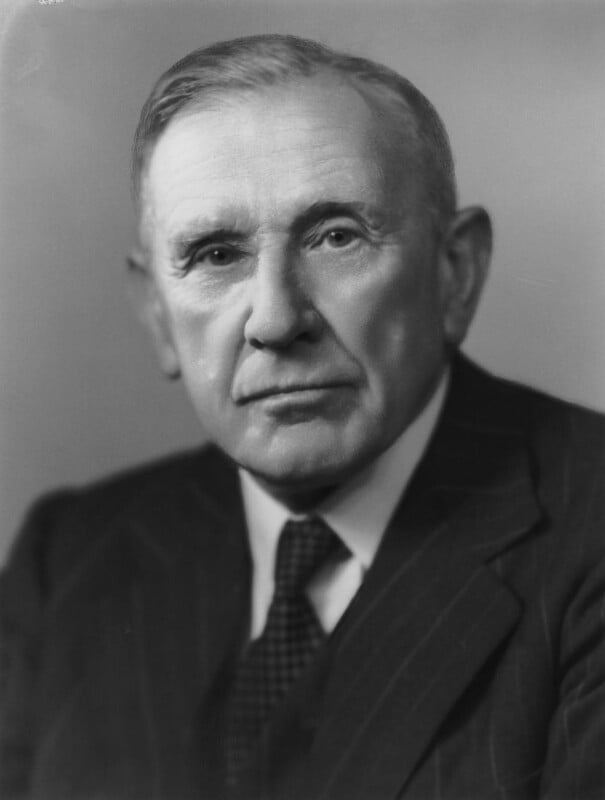
\includegraphics[height=0.42\textheight]{ch10_hurst_1953.jpg}\\[1mm]
\imgcap{Harold Edwin Hurst, 1953}
\imgcredit{https://commons.wikimedia.org/wiki/File:Harold_Edwin_Hurst_in_1953.jpg}{Foto: Elliott \& Fry (1953); domeniu public; Wikimedia Commons}
\end{column}
\begin{column}{0.62\textwidth}
\begin{itemize}
    \item Hurst a studiat secole de niveluri ale Nilului pentru a dimensiona rezervoarele de deasupra Aswanului \refHur
    \item Amplitudinea ajustată a afluxurilor cumulate creștea ca $n^H$ cu $H \approx 0{,}7$, nu ca $n^{1/2}$: \textbf{efectul Hurst}
    \item Anii ploioși urmează anilor ploioși în serii lungi: o dependență pe care niciun ARMA finit nu o reproduce
    \item Au urmat două explicații
    \begin{itemize}
        \item zgomotul gaussian fracționar \refMVN
        \item diferențierea fracționară \refGJ, \refHos
    \end{itemize}
\end{itemize}
\end{column}
\end{columns}
\end{frame}

\begin{frame}{Înregistrările fluviului}
\itemsize{\small}
\begin{columns}[T]
\begin{column}{0.34\textwidth}
\centering
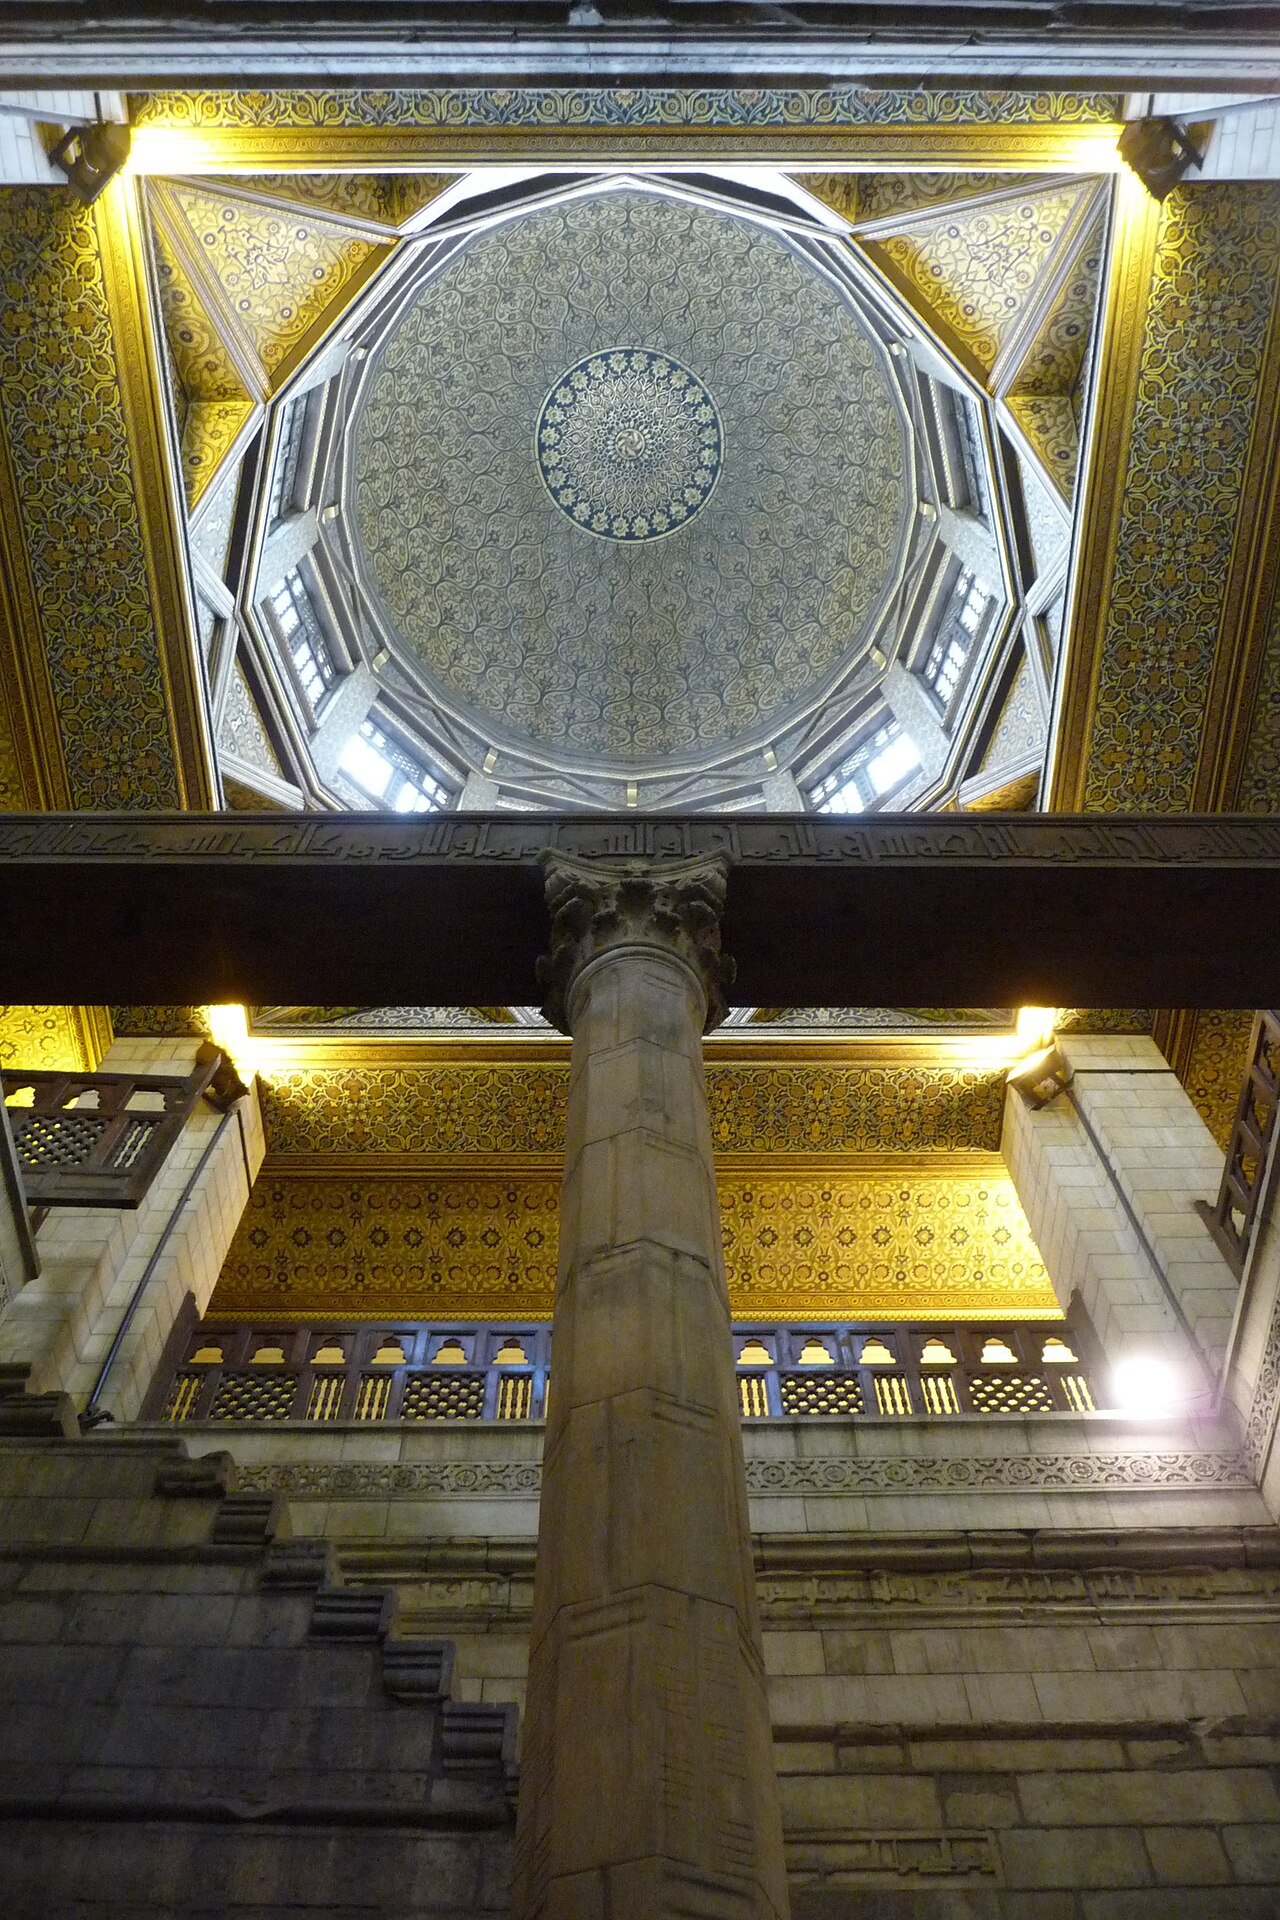
\includegraphics[height=0.5\textheight]{ch10_nilometer_2009.jpg}\\[1mm]
\imgcap{Nilometrul de pe insula Roda, Cairo}
\imgcredit{https://commons.wikimedia.org/wiki/File:Nilometer._Roda_Innen.JPG}{Foto: Willyman (2009); CC BY-SA 4.0; Wikimedia Commons}
\end{column}
\begin{column}{0.64\textwidth}
\begin{itemize}
    \item Nilometrul de pe Roda a înregistrat minimele anuale ale Nilului începînd cu secolul al VII-lea: una dintre cele mai vechi serii de timp
    \item Aceste minime sînt setul clasic de date cu memorie lungă \refBFGK
    \item Azi aceeași întrebare se pune pentru volatilitate, inflație și dobînzi: se stinge un șoc geometric sau hiperbolic?
    \item Și una mai nouă: pe orizonturi scurte, este volatilitatea mai netedă sau mai neregulată decît mișcarea browniană?
\end{itemize}
\end{column}
\end{columns}
\end{frame}

\begin{frame}{Douăzeci și doi de ani de logaritm al varianței realizate}
\itemsize{\footnotesize}
\begin{center}
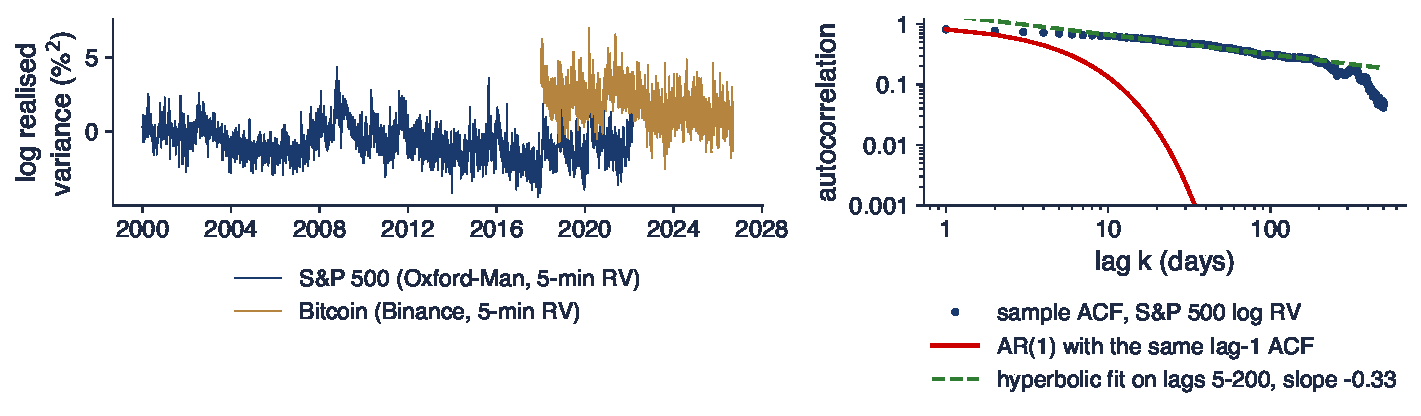
\includegraphics[width=0.97\textwidth,height=0.5\textheight,keepaspectratio]{ats_ch10_overview.pdf}
\end{center}
\vspace{-0.25cm}
\begin{itemize}
    \item Stînga: S\&P 500 (Oxford-Man, $n = 5\,552$ zile pînă la 25 februarie 2022) și Bitcoin ($n = 3\,165$ zile pînă la 18 septembrie 2026); dreapta: ACF de eșantion a logaritmului RV pentru S\&P 500, laguri 1--500, scară log-log
\end{itemize}
\quantlet{ATS\_ch10\_memory}{\qlurl{ATS_ch10_memory}}
\end{frame}

\begin{frame}{Interpretarea imaginii de ansamblu}
\itemsize{\small}
\begin{itemize}
    \item ACF 0{,}82 la lagul 1, 0{,}53 la 22, încă 0{,}18 la 250: un AR(1) cu același prim lag ar da circa $10^{-22}$ la lagul 250
    \item Pe lagurile 5--200, ACF este o dreaptă în scara log-log, cu panta \ensuremath{-}0{,}33: o descreștere hiperbolică $k^{2d-1}$ cu $d \approx 0{,}34$
    \item Estimația local Whittle este mai mare, 0{,}62: sub memorie lungă, ACF de eșantion este deplasată în jos la laguri mari
    \item Restul capitolului întreabă în care dintre aceste cifre putem avea încredere și de ce aceeași serie pare și neregulată
\end{itemize}
\end{frame}


%=============================================================================
\section{Memoria lungă: caracterizare spectrală}
%=============================================================================

\begin{frame}{Cunoscut din TSA și elemente noi}
\itemsize{\small}
\begin{itemize}
    \item Cunoscut (\atschlink{https://danpele.github.io/Time-Series-Analysis/RO/Cursuri/capitol8_memorie_lunga_arfima.pdf}{TSA, Capitolul 8}): diferențierea fracționară, ARFIMA$(p,d,q)$, R/S și DFA, GPH și local Whittle ca rețete, FIGARCH și HAR pe scurt, memoria lungă aparentă prin exemple
    \item Nou: teoria din spatele rețetelor
    \begin{itemize}
        \item definiții echivalente, agregare, varianța mediei de eșantion
        \item legile limită ale estimatorilor semiparametrici, $d$ nestaționar, deplasarea și alegerea lui $m$
        \item un test formal împotriva salturilor de nivel; cointegrarea fracționară; rough volatility
    \end{itemize}
    \item Replicări: agregarea Granger (1980), schema Qu (2011), scalarea Gatheral, Jaisson și Rosenbaum (2018, secțiunea 2) pe datele Oxford-Man folosite de ei
\end{itemize}
\end{frame}

\begin{frame}{Două definiții ale memoriei lungi (1/2)}
\itemsize{\small}
\begin{itemize}
    \item \textbf{Domeniul timpului}: autocovarianțele scad hiperbolic și nu sînt sumabile
    \[ \gamma(k) \sim c_\gamma\,k^{2d-1} \ \ (k \to \infty), \quad 0 < d < 1/2 \ \Rightarrow\ \sum_k|\gamma(k)| = \infty \]
    \begin{itemize}
        \item $\gamma(k)$: autocovarianța la lagul $k$; $d$: parametrul de memorie; $c_\gamma > 0$: o constantă; $a_k \sim b_k$ înseamnă $a_k/b_k \to 1$
        \item memorie scurtă: $\sum_k|\gamma(k)| < \infty$ (de exemplu ARMA, cu descreștere geometrică)
    \end{itemize}
    \item \textbf{Domeniul frecvenței}: densitatea spectrală are un pol în frecvența zero
    \[ f(\lambda) \sim c_f\,\lambda^{-2d} \quad (\lambda \to 0^+) \]
    \begin{itemize}
        \item $f(\lambda)$: densitatea spectrală la frecvența $\lambda \in (0, \pi]$; $c_f > 0$: o constantă
        \item $d < 0$: antipersistență, $f(0) = 0$, $\sum_k\gamma(k) = 0$; $d = 0$: memorie scurtă
    \end{itemize}
\end{itemize}
\end{frame}

\begin{frame}{Două definiții ale memoriei lungi (2/2)}
\itemsize{\small}
\begin{itemize}
    \item Echivalența: pentru $\gamma$ cvasi-monotonă, constantele sînt legate (teoreme abeliene--tauberiene) \refBFGK
    \[ c_f = c_\gamma\,\Gamma(2d)\,\frac{\sin(\pi/2 - \pi d)}{\pi} \]
    \begin{itemize}
        \item $\Gamma(\cdot)$: funcția gamma; fără această regularitate, cele două definiții diferă
        \item estimatorii semiparametrici folosesc doar definiția din domeniul frecvenței
    \end{itemize}
    \item Scara Hurst: $H = d + 1/2$ pentru seria staționară
    \begin{itemize}
        \item $H > 1/2$: persistentă; $H < 1/2$: antipersistentă; $H = 1/2$: memorie scurtă
    \end{itemize}
\end{itemize}
\end{frame}

\begin{frame}{Integrarea fracționară și ARFIMA (1/2)}
\itemsize{\small}
\begin{itemize}
    \item Operatorul de diferențiere fracționară este o serie de puteri în operatorul lag $L$ ($LX_t = X_{t-1}$) \refGJ, \refHos
    \[ (1 - L)^d = \sum_{k\ge0}\pi_k L^k, \qquad \pi_0 = 1, \quad \pi_k = \pi_{k-1}\frac{k - 1 - d}{k}, \quad \pi_k \sim \frac{k^{-d-1}}{\Gamma(-d)} \]
    \begin{itemize}
        \item $\pi_k$: ponderea lui $X_{t-k}$; scade hiperbolic, deci filtrul are memorie infinită; $d = 1$ dă diferența obișnuită $1 - L$
    \end{itemize}
    \item ARFIMA$(p,d,q)$: un ARMA pentru seria diferențiată fracționar
    \[ \phi(L)(1 - L)^d(X_t - \mu) = \theta(L)\varepsilon_t \]
    \begin{itemize}
        \item $\phi(L)$, $\theta(L)$: polinoamele AR și MA de ordinele $p$, $q$; $\mu$: media; $\varepsilon_t$: zgomot alb cu varianța $\sigma^2$
        \item staționar și inversabil pentru $-1/2 < d < 1/2$
    \end{itemize}
\end{itemize}
\end{frame}

\begin{frame}{Integrarea fracționară și ARFIMA (2/2)}
\itemsize{\small}
\begin{itemize}
    \item Spectrul: un pol în zero înmulțit cu spectrul părții ARMA
    \[ f(\lambda) = \frac{\sigma^2}{2\pi}\,\big|2\sin(\lambda/2)\big|^{-2d}\,\frac{|\theta(e^{-i\lambda})|^2}{|\phi(e^{-i\lambda})|^2} = |2\sin(\lambda/2)|^{-2d}f^*(\lambda) \]
    \begin{itemize}
        \item $f^*$: partea netedă de memorie scurtă (ARMA); lîngă zero $|2\sin(\lambda/2)| \approx \lambda$, deci $f(\lambda) \approx f^*(0)\lambda^{-2d}$
    \end{itemize}
    \item ARFIMA$(0,d,0)$: varianța și autocorelațiile în formă închisă
    \[ \gamma(0) = \sigma^2\frac{\Gamma(1 - 2d)}{\Gamma(1 - d)^2}, \qquad \rho(k) = \frac{\Gamma(k + d)\Gamma(1 - d)}{\Gamma(k - d + 1)\Gamma(d)} \sim \frac{\Gamma(1 - d)}{\Gamma(d)}k^{2d-1} \]
    \begin{itemize}
        \item recursia $\rho(k) = \rho(k - 1)\,(k - 1 + d)/(k - d)$, $\rho(1) = d/(1 - d)$
    \end{itemize}
\end{itemize}
\end{frame}

\begin{frame}{Descreștere hiperbolică și geometrică}
\itemsize{\footnotesize}
\begin{center}
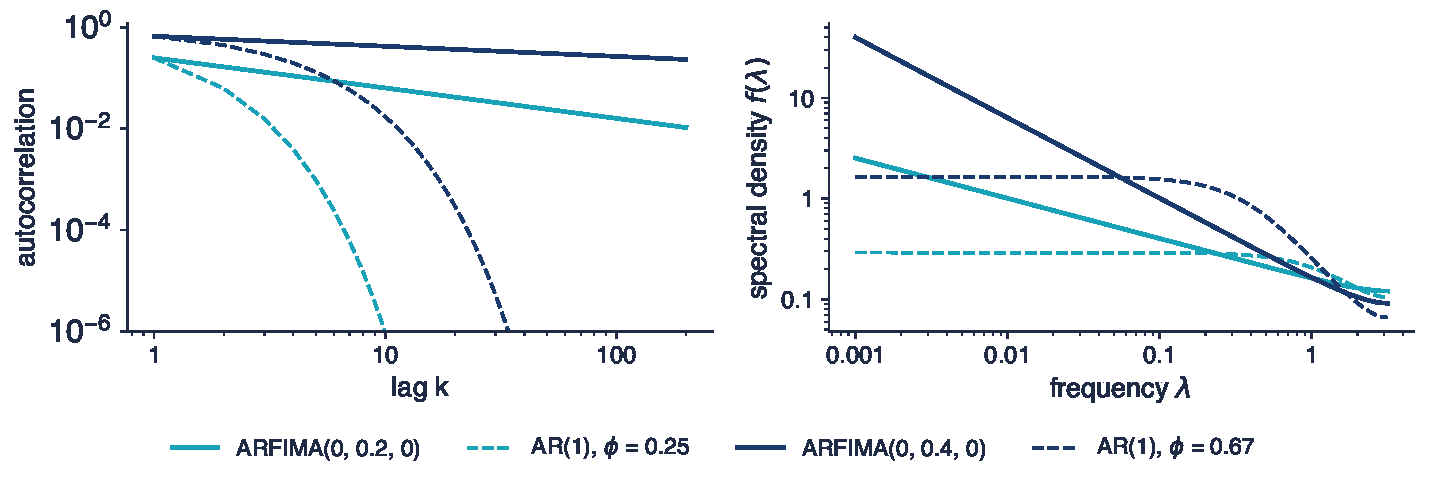
\includegraphics[width=0.97\textwidth,height=0.5\textheight,keepaspectratio]{ats_ch10_acf_spec.pdf}
\end{center}
\vspace{-0.25cm}
\begin{itemize}
    \item Stînga: ACF pentru ARFIMA$(0,d,0)$ și pentru un AR(1) cu același $\rho(1)$, scară log-log; dreapta: densitățile spectrale lîngă zero, AR(1) scalat la aceeași varianță
\end{itemize}
\quantlet{ATS\_ch10\_memory}{\qlurl{ATS_ch10_memory}}
\end{frame}

\begin{frame}{Interpretarea celor două descreșteri}
\itemsize{\small}
\begin{itemize}
    \item $d = 0{,}4$: $\rho(1) = 0{,}667$, $\rho(10) = 0{,}424$, $\rho(100) = 0{,}267$; AR(1) corespunzător are $\rho(100)$ de ordinul $10^{-18}$
    \item Sumele parțiale $\sum_{k\le100}\rho(k) = 33{,}0$ și $\sum_{k\le200}\rho(k) = 57{,}8$: continuă să crească, precum $K^{2d}$
    \item În spectru diferența este un pol față de un platou: memoria lungă se află la frecvențele cele mai joase, unde există puține ordonate ale periodogramei
    \item De aceea toți estimatorii semiparametrici privesc doar cele mai joase $m$ frecvențe Fourier
\end{itemize}
\end{frame}

\begin{frame}{Originea memoriei lungi: agregarea}
\itemsize{\small}
\begin{itemize}
    \item \refGra: suma scalată a $N$ serii AR(1) independente, cu coeficienți aleatori
    \[ X_t = \frac{1}{\sqrt N}\sum_{i=1}^N x_{it}, \qquad x_{it} = \phi_i x_{i,t-1} + \varepsilon_{it}, \qquad \phi_i^2 \sim \mathrm{Beta}(p, q) \]
    \begin{itemize}
        \item $\phi_i$: persistența unității $i$, extrasă o singură dată; densitatea Beta $\propto \phi^{2p-1}(1 - \phi^2)^{q-1}$ pe $(0, 1)$; $q$ controlează masa din apropierea rădăcinii unitare
    \end{itemize}
    \item Derivare: mediem autocovarianțele AR(1) după distribuția lui $\phi$
    \[ \gamma_X(k) = \E\Big[\frac{\phi^k}{1 - \phi^2}\Big] \propto \int_0^1\phi^{k+2p-1}(1 - \phi^2)^{q-2}d\phi \propto B\Big(\frac{k}{2} + p, q - 1\Big) \sim c\,k^{-(q-1)} \]
    \begin{itemize}
        \item $B(\cdot, \cdot)$: funcția beta; identificînd cu $k^{2d-1}$ obținem $d = 1 - q/2$, memorie lungă pentru $1 < q < 2$
    \end{itemize}
    \item Lectura economică: inflația, volatilitatea sau producția agregată combină mulți agenți cu memorie scurtă și persistență eterogenă; cîteva unități apropiate de rădăcina unitară domină frecvențele joase
    \item Memoria lungă poate fi deci structurală, nu o curiozitate a estimatorului
\end{itemize}
\end{frame}

\begin{frame}{Agregarea seriilor AR(1)}
\itemsize{\footnotesize}
\begin{center}
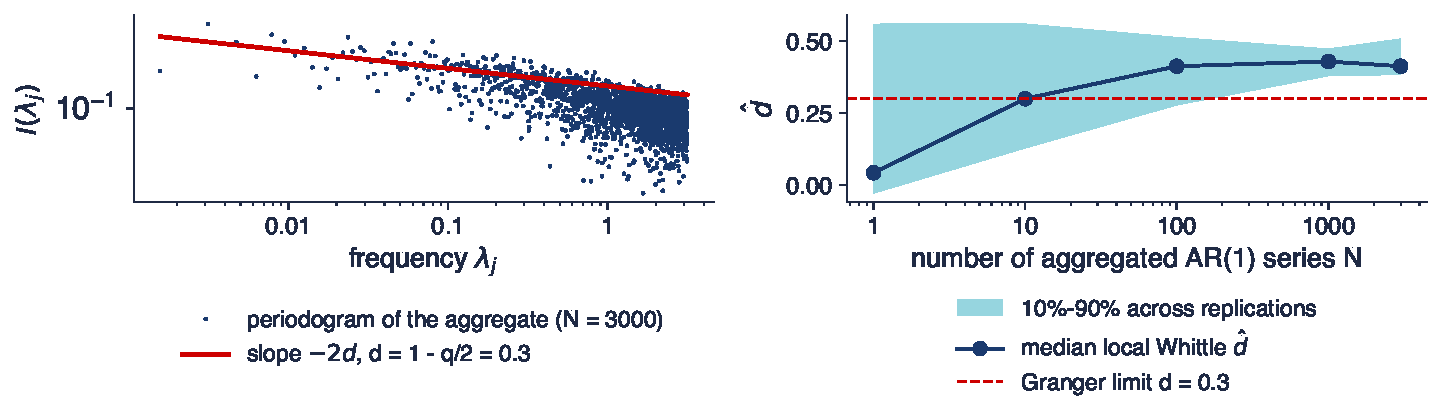
\includegraphics[width=0.97\textwidth,height=0.5\textheight,keepaspectratio]{ats_ch10_aggregation.pdf}
\end{center}
\vspace{-0.25cm}
\begin{itemize}
    \item $\phi_i^2 \sim \mathrm{Beta}(1; 1{,}4)$, deci $d = 1 - q/2 = 0{,}3$; $n = 4000$; local Whittle cu $m = 219$, 20 replicări pentru fiecare $N$; stînga: periodograma unui agregat de 3000 de serii
\end{itemize}
\quantlet{ATS\_ch10\_memory}{\qlurl{ATS_ch10_memory}}
\end{frame}

\begin{frame}{Interpretarea agregării}
\itemsize{\small}
\begin{itemize}
    \item Un singur AR(1): mediana $\hat d = 0{,}04$; zece serii: 0{,}30; 100 de serii: 0{,}41; 3000 de serii: 0{,}41 (10\%--90\%: între 0{,}38 și 0{,}51)
    \item Estimația se stabilizează peste limita 0{,}3: spectrul agregatului este $\lambda^{-2d}$ doar foarte aproape de zero, iar $m = n^{0{,}65}$ intră în zona în care nu mai este
    \item Aceasta este problema deplasării din secțiunea 2 în forma ei cea mai pură: un estimator semiparametric este atît de bun cît îi este lățimea de bandă
    \item Direcția efectului, de la lipsa memoriei la memorie lungă clară, este esența teoremei lui Granger
\end{itemize}
\end{frame}

\begin{frame}{Consecințe pentru inferență: media de eșantion}
\itemsize{\small}
\begin{itemize}
    \item Varianța mediei de eșantion $\bar X_n$ scade mai lent decît $1/n$
    \[ \Var(\bar X_n) = \frac1n\sum_{|k|<n}\Big(1 - \frac{|k|}{n}\Big)\gamma(k) \sim \frac{c_\gamma}{d(2d + 1)}\,n^{2d-1} \]
    \begin{itemize}
        \item media converge cu viteza $n^{1/2-d}$, nu $n^{1/2}$; cu $d = 0{,}4$: $n^{0{,}1}$
    \end{itemize}
    \item Erorile standard HAC (\atschlink{https://danpele.github.io/Advanced-Time-Series/RO/Cursuri/capitol0_recapitulare_inferenta.pdf}{Capitolul 0}) presupun $\sum_k|\gamma(k)| < \infty$: sub memorie lungă, varianța de termen lung este infinită, iar intervalele Newey--West sînt prea înguste
    \begin{itemize}
        \item la fel pentru testele DM (\atschlink{https://danpele.github.io/Advanced-Time-Series/RO/Cursuri/capitol1_evaluarea_prognozelor.pdf}{Capitolul 1}) aplicate diferențelor de pierderi care moștenesc memoria lungă
    \end{itemize}
    \item Regresie cu regresori și erori cu memorie lungă: pantele OLS converg încet
    \begin{itemize}
        \item regresie falsă între serii fracționare independente cînd $d_x + d_u > 1/2$ ($d_x$, $d_u$: memoria regresorului și a erorii)
    \end{itemize}
    \item Fiecare test din acest curs construit pe asimptotica $\sqrt n$ trebuie reexaminat cînd $d > 0$
\end{itemize}
\end{frame}

\begin{frame}{Recapitulare: memoria lungă}
\itemsize{\small}
\begin{itemize}
    \item Memoria lungă: ACF hiperbolică $k^{2d-1}$ și un pol spectral $\lambda^{-2d}$; $H = d + 1/2$
    \item ARFIMA separă polul $|2\sin(\lambda/2)|^{-2d}$ de partea de memorie scurtă $f^*$
    \item Agregarea unităților AR(1) eterogene produce memorie lungă; media converge cu $n^{1/2-d}$
\end{itemize}
\end{frame}


%=============================================================================
\section{Estimarea semiparametrică și asimptotica ei}
%=============================================================================

\begin{frame}{Periodograma lîngă frecvența zero}
\itemsize{\small}
\begin{itemize}
    \item Periodograma: pătratul modulului transformatei Fourier discrete, la frecvențele Fourier
    \[ I(\lambda_j) = \frac{1}{2\pi n}\Big|\sum_{t=1}^n X_te^{-i\lambda_jt}\Big|^2, \qquad \lambda_j = \frac{2\pi j}{n}, \quad j = 1, \dots, m \]
    \begin{itemize}
        \item $n$: mărimea eșantionului; $m$: lățimea de bandă, numărul frecvențelor celor mai joase folosite; memorie scurtă: $I(\lambda_j)/f(\lambda_j)$ asimptotic i.i.d.\ $\mathrm{Exp}(1)$
    \end{itemize}
    \item Memorie lungă: pentru $j$ fix, $\E\,I(\lambda_j)/f(\lambda_j) \not\to 1$, iar ordonatele rămîn corelate \refRobB
    \begin{itemize}
        \item distorsiunea dispare cînd $j \to \infty$: demonstrațiile cer $m \to \infty$, $m/n \to 0$ și tratează separat primele frecvențe
    \end{itemize}
    \item Modelul semiparametric: se specifică doar comportamentul lîngă zero
    \[ f(\lambda) = G\lambda^{-2d}\big(1 + O(\lambda^\beta)\big), \qquad \lambda \to 0, \quad \beta \in (0, 2] \]
    \begin{itemize}
        \item $G > 0$: nivelul spectrului la frecvențe joase; $\beta$: netezimea restului; $\beta = 2$ pentru ARFIMA, deoarece $f^*$ este netedă și pară
    \end{itemize}
\end{itemize}
\end{frame}

\begin{frame}{GPH: regresia pe logaritmul periodogramei}
\itemsize{\small}
\begin{itemize}
    \item Logaritmînd $I = f\xi$ obținem o regresie liniară în $\log\lambda_j$, cu panta $-2d$ \refGPH
    \[ \log I(\lambda_j) = \log G - 2d\log\lambda_j + \log\xi_j, \qquad \xi_j = \frac{I(\lambda_j)}{f(\lambda_j)} \]
    \begin{itemize}
        \item OLS pe $j = 1, \dots, m$; cu $\xi_j \sim \mathrm{Exp}(1)$: $\E\log\xi_j = -\gamma_E$ ($\gamma_E \approx 0{,}577$, constanta lui Euler), $\Var\log\xi_j = \pi^2/6$
    \end{itemize}
    \item \refRobB: pentru $|d| < 1/2$ și $X$ gaussian, dacă $m \to \infty$ și $m^5/n^4 \to 0$
    \[ \sqrt m(\hat d_{GPH} - d) \to N(0, \pi^2/24) \]
    \begin{itemize}
        \item originea lui $\pi^2/24$: $\Var(\hat d) = \dfrac{\pi^2/6}{4\sum_j\nu_j^2}$, cu $\nu_j = \log j - \overline{\log j}$ regresorul centrat și $\sum_j\nu_j^2 \sim m$
    \end{itemize}
    \item Deplasarea pentru ARFIMA \refHDB: $\E\hat d - d \approx -\dfrac{2\pi^2}{9}\dfrac{f^{*\prime\prime}(0)}{f^*(0)}\dfrac{m^2}{n^2}$
    \begin{itemize}
        \item condiția $m^5/n^4 \to 0$ face deplasarea neglijabilă față de abaterea standard $m^{-1/2}$
    \end{itemize}
\end{itemize}
\end{frame}

\begin{frame}{Local Whittle (1/2): funcția obiectiv}
\itemsize{\small}
\begin{itemize}
    \item Aproximarea Whittle a log-verosimilității gaussiene, restrînsă la $j \le m$, cu $f(\lambda_j) = G\lambda_j^{-2d}$
    \[ Q(G, d) = \frac1m\sum_{j=1}^m\Big[\log\big(G\lambda_j^{-2d}\big) + \frac{I(\lambda_j)}{G\lambda_j^{-2d}}\Big] \]
    \begin{itemize}
        \item aceeași formă ca QLIKE (\atschlink{https://danpele.github.io/Advanced-Time-Series/RO/Cursuri/capitol8_volatilitate_avansata.pdf}{Capitolul 8}): spectrul modelului $G\lambda_j^{-2d}$ este ajustat la periodogramă, ordonată cu ordonată
    \end{itemize}
    \item Eliminăm $G$ prin concentrare \refRobC: pentru $d$ dat, nivelul optim este media lui $\lambda_j^{2d}I(\lambda_j)$
    \[ \hat G(d) = \frac1m\sum_j\lambda_j^{2d}I(\lambda_j), \qquad \hat d_{LW} = \arg\min_d R(d) \]
    \[ R(d) = \log\hat G(d) - \frac{2d}{m}\sum_{j=1}^m\log\lambda_j \]
    \begin{itemize}
        \item o minimizare unidimensională în $d$
    \end{itemize}
\end{itemize}
\end{frame}

\begin{frame}{Local Whittle (2/2): varianța}
\itemsize{\small}
\begin{itemize}
    \item Scorul în valoarea adevărată: o sumă ponderată de $\xi_j - 1$
    \[ R'(d) = \frac{2}{m}\sum_j\nu_j\Big(\frac{\lambda_j^{2d}I(\lambda_j)}{\hat G(d)} - 1\Big) \]
    \begin{itemize}
        \item $\nu_j = \log\lambda_j - \overline{\log\lambda}$: logaritmul centrat al frecvenței; cu $\Var(\xi_j) = 1$ și $R''(d) \to 4$: $\sqrt m(\hat d - d) \to N(0, 4/16) = N(0, 1/4)$
    \end{itemize}
    \item Nicio ipoteză de distribuție în afara unui proces liniar cu inovații diferențe de martingal
    \begin{itemize}
        \item eficiența relativă față de GPH: $(\pi^2/24)/(1/4) = \pi^2/6 \approx 1{,}64$
        \item derivarea pas cu pas: \atsapplink{atsapp1}{atssrc1}{Anexa}  % applink: varianța estimatorului local Whittle
    \end{itemize}
\end{itemize}
\end{frame}

\begin{frame}{Local Whittle: teorema și limitele ei}
\itemsize{\small}
\begin{itemize}
    \item \refRobC: pentru $d \in (-1/2, 1/2)$, $f(\lambda) = G\lambda^{-2d}(1 + O(\lambda^\beta))$ și o lățime de bandă cu $1/m + m^{1+2\beta}(\log m)^2/n^{2\beta} \to 0$
    \begin{itemize}
        \item $\hat d \to_p d$ și $\sqrt m(\hat d - d) \to N(0, 1/4)$; condiția pentru $m$: crește, dar suficient de lent pentru ca deplasarea să dispară
    \end{itemize}
    \item $d$ nestaționar: consistent pentru $d < 1$, asimptotic normal pentru $d < 3/4$ \refVel
    \begin{itemize}
        \item pentru $d > 1$ converge în probabilitate la 1; între $3/4$ și 1 limita nu este normală \refPS
    \end{itemize}
    \item Remedii: diferențiem întîi datele (trebuie să știm că $d > 1/2$), aplicăm o fereastră periodogramei (cu cost în varianță) sau estimăm exact
\end{itemize}
\end{frame}

\begin{frame}{Local Whittle exact}
\itemsize{\small}
\begin{itemize}
    \item \refSP: înlocuim $\lambda_j^{2d}I_X(\lambda_j)$ prin periodograma datelor diferențiate fracționar
    \[ \Delta^dX_t = \sum_{k=0}^{t-1}\pi_kX_{t-k}, \qquad R_E(d) = \log\Big(\frac1m\sum_jI_{\Delta^dX}(\lambda_j)\Big) - \frac{2d}{m}\sum_j\log\lambda_j \]
    \begin{itemize}
        \item $\Delta^d = (1 - L)^d$, trunchiat la începutul eșantionului; $I_{\Delta^dX}$: periodograma seriei diferențiate
        \item $\lambda^{2d}I_X(\lambda)$ aproximează $I_{\Delta^dX}(\lambda)$ doar pentru $d < 1/2$; versiunea exactă elimină eroarea care strică LW pentru $d$ mare: $\sqrt m(\hat d_{ELW} - d) \to N(0, 1/4)$ pe orice interval de căutare de lățime $< 9/2$
    \end{itemize}
    \item Media necunoscută \refShi: se scade $\hat\mu(d) = w(d)\bar X + (1 - w(d))X_1$
    \begin{itemize}
        \item $w(d) = 1$ pentru $d \le 1/2$, $0$ pentru $d \ge 3/4$, netedă între ele: media de eșantion estimează prost nivelul cînd $d > 1/2$
    \end{itemize}
    \item Costul: o diferență fracționară pentru fiecare evaluare, $O(n\log n)$ prin FFT
\end{itemize}
\end{frame}

\begin{frame}{GPH, local Whittle și local Whittle exact prin Monte Carlo}
\itemsize{\footnotesize}
\begin{center}
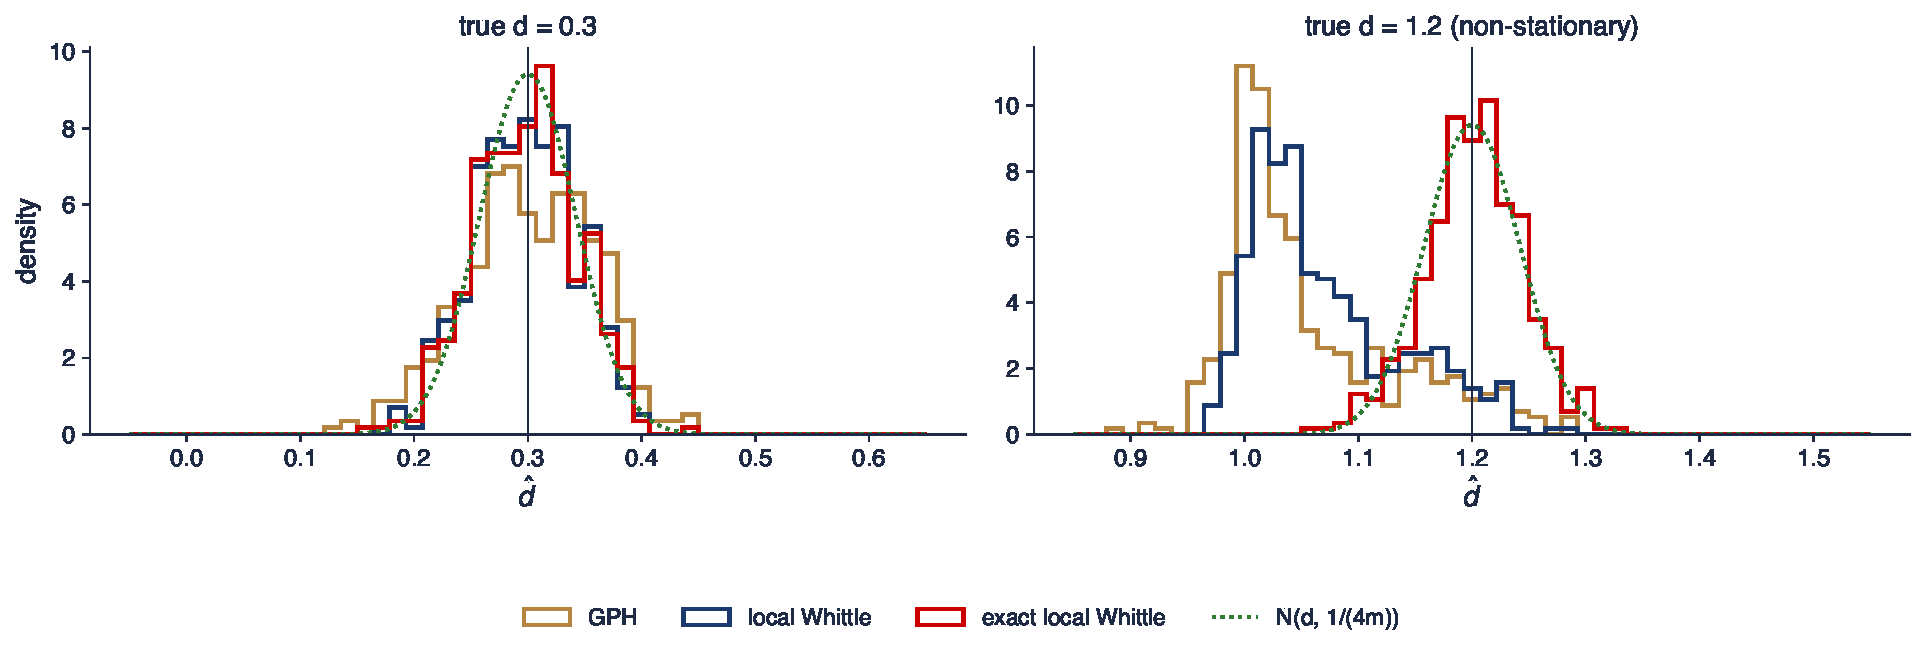
\includegraphics[width=0.97\textwidth,height=0.5\textheight,keepaspectratio]{ats_ch10_mc_estimators.pdf}
\end{center}
\vspace{-0.25cm}
\begin{itemize}
    \item 400 de traiectorii ARFIMA$(0,d,0)$ gaussiene, $n = 2000$, $m = n^{0{,}65} = 139$; abaterea standard asimptotică: GPH 0{,}054, local Whittle 0{,}042; $d = 1{,}2$ se simulează ca sumă parțială a unui ARFIMA$(0; 0{,}2; 0)$
\end{itemize}
\quantlet{ATS\_ch10\_estimation}{\qlurl{ATS_ch10_estimation}}
\end{frame}

\begin{frame}{Interpretarea experimentului Monte Carlo}
\itemsize{\small}
\begin{itemize}
    \item $d = 0{,}3$: medii 0{,}301; 0{,}297; 0{,}298; abateri standard 0{,}057; 0{,}045; 0{,}045; acoperirea de 95\%: 94\%, 94\%, 95\% (GPH, LW, ELW)
    \item Legile asimptotice sînt precise la $n = 2000$; local Whittle este de circa $\sqrt{\pi^2/6}$ ori mai strîns decît GPH
    \item $d = 1{,}2$: GPH 1{,}057 și LW 1{,}072 se strîng spre 1 (acoperire 26\% și 22\%); ELW 1{,}202, acoperire 93\%
    \item Pentru seriile care pot fi nestaționare (prețuri, inflația în nivel, logaritmul RV cu $d$ aproape de 0,5) raportați ELW
\end{itemize}
\end{frame}

\begin{frame}{Lățimea de bandă: deplasare și varianță}
\itemsize{\small}
\begin{itemize}
    \item Deplasarea principală (GPH și LW): curbura lui $\log f^*$ lîngă zero trece în pantă
    \[ \E\hat d - d \approx -\frac{2\pi^2}{9}\,\frac{f^{*\prime\prime}(0)}{f^*(0)}\Big(\frac mn\Big)^2 = C\Big(\frac mn\Big)^2 \]
    \begin{itemize}
        \item din regresia lui $\log f^*(\lambda_j) \approx \log f^*(0) + b\lambda_j^2$, $b = \tfrac12f^{*\prime\prime}(0)/f^*(0)$, pe $-2\nu_j$; $C$: constanta deplasării
        \item ARFIMA$(1,d,0)$: $f^{*\prime\prime}(0)/f^*(0) = -2\phi/(1 - \phi)^2$, deplasare în sus pentru $\phi > 0$
    \end{itemize}
    \item MSE: pătratul deplasării plus varianța; minimizarea în $m$ dă lățimea de bandă optimă \refHR
    \[ \mathrm{MSE}(m) \approx C^2\Big(\frac mn\Big)^4 + \frac{1}{4m}, \qquad m^* = \Big(\frac{n^4}{16C^2}\Big)^{1/5} \propto n^{4/5} \]
    \begin{itemize}
        \item $C$ este necunoscută: regulile plug-in o estimează; local Whittle polinomial \refAnSu\ elimină termenul în $\lambda^2$ cu un cost în varianță
    \end{itemize}
    \item La $m^*$ deplasarea și abaterea standard sînt de același ordin, deci intervalele nominale acoperă prea puțin; în practică: graficul lui $\hat d(m)$ pe un interval de valori, raportat împreună cu intervalele
\end{itemize}
\end{frame}

\begin{frame}{Deplasarea și RMSE în funcție de lățimea de bandă}
\itemsize{\footnotesize}
\begin{center}
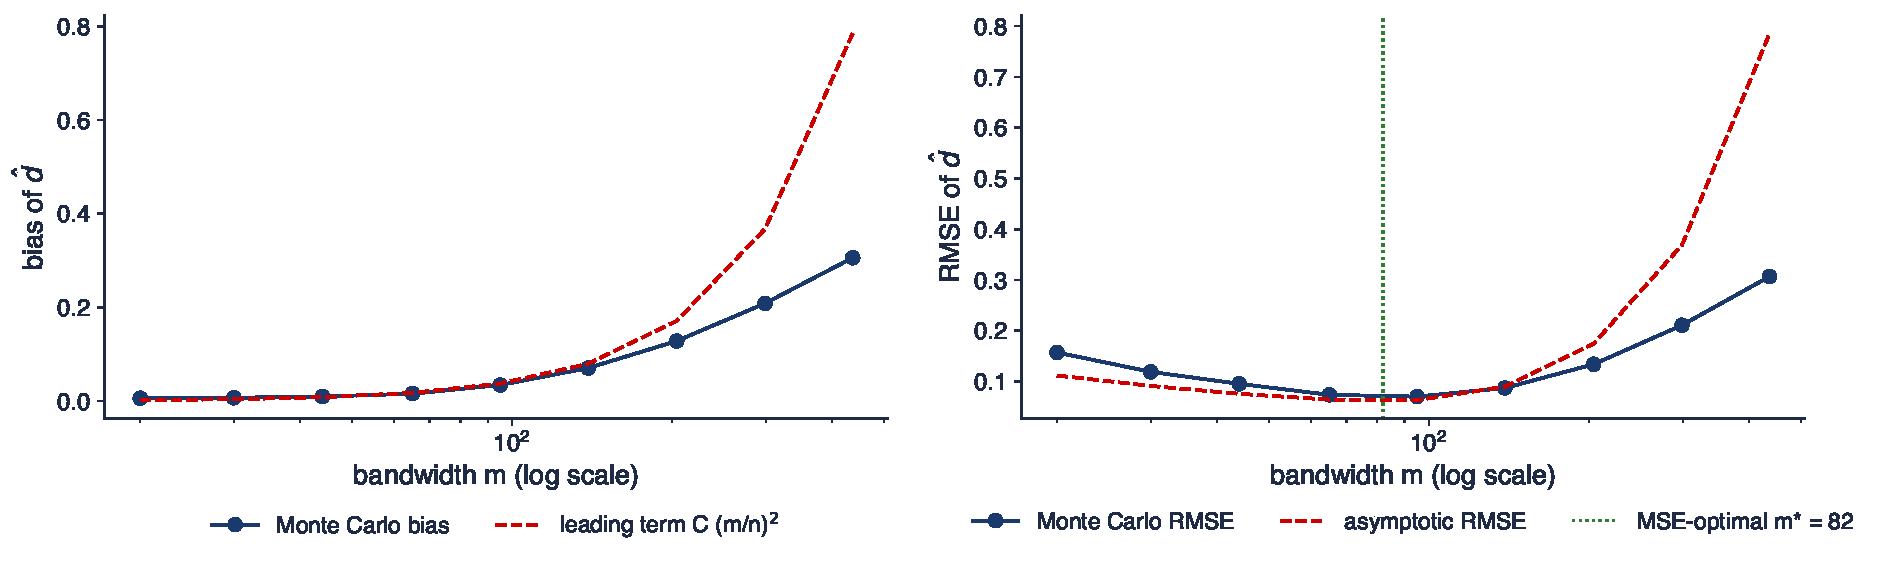
\includegraphics[width=0.97\textwidth,height=0.5\textheight,keepaspectratio]{ats_ch10_bandwidth.pdf}
\end{center}
\vspace{-0.25cm}
\begin{itemize}
    \item Local Whittle, ARFIMA$(1; 0{,}3; 0)$ cu $\phi = 0{,}6$, $n = 2000$, 300 de replicări, $m = n^a$ pentru $a = 0{,}40, \dots, 0{,}80$; linie întreruptă: deplasarea principală $C(m/n)^2$ cu $C = 16{,}4$ și RMSE asimptotic
\end{itemize}
\quantlet{ATS\_ch10\_estimation}{\qlurl{ATS_ch10_estimation}}
\end{frame}

\begin{frame}{Interpretarea compromisului lățimii de bandă}
\itemsize{\small}
\begin{itemize}
    \item $m$ mic ($a = 0{,}40$): deplasare 0{,}006, RMSE 0{,}16, dominat de varianță; $m$ mare ($a = 0{,}80$): deplasare 0{,}31, RMSE 0{,}31
    \item Cel mai mic RMSE Monte Carlo, 0{,}070, la $m = 95$ ($a = 0{,}60$); teoria: $m^* = 82$ ($a = 0{,}58$)
    \item Termenul principal supraestimează deplasarea la $m$ mare (0{,}79 față de 0{,}31): dezvoltarea în $\lambda^2$ este locală
    \item O regulă fixă precum $m = n^{0{,}8}$ poate transforma o componentă AR de memorie scurtă în memorie lungă aparentă
\end{itemize}
\end{frame}

\begin{frame}{Alternativa parametrică: Whittle și ML exact}
\itemsize{\small}
\begin{itemize}
    \item Whittle: se ajustează o densitate spectrală complet specificată pe toate frecvențele \refFT
    \[ \hat\vartheta = \arg\min_\vartheta\sum_{j=1}^{\lfloor (n-1)/2\rfloor}\Big[\log f(\lambda_j; \vartheta) + \frac{I(\lambda_j)}{f(\lambda_j; \vartheta)}\Big] \]
    \begin{itemize}
        \item $\vartheta$: toți parametrii ARFIMA$(p,d,q)$ ($d$, coeficienții AR și MA, $\sigma^2$); consistent cu viteza $\sqrt n$ și eficient dacă modelul este corect; $\Var(\hat d) \approx 6/(\pi^2n)$ pentru $(0,d,0)$
    \end{itemize}
    \item Compromisul este între robustețe și eficiență: un $(p, q)$ greșit deplasează $\hat d$ pentru orice $n$
    \begin{itemize}
        \item semiparametric: viteza $\sqrt m$, robust la $f^*$; parametric: viteza $\sqrt n$, expus la specificarea greșită
    \end{itemize}
    \item Practica obișnuită: întîi $\hat d$ semiparametric, apoi un model parametric al cărui $d$ cade în intervalul lui, apoi prognoze
\end{itemize}
\end{frame}

\begin{frame}{Recapitulare: estimarea semiparametrică}
\itemsize{\small}
\begin{itemize}
    \item GPH: $N(d, \pi^2/(24m))$; local Whittle: $N(d, 1/(4m))$; local Whittle exact păstrează $N(d, 1/(4m))$ pentru $d$ nestaționar
    \item Deplasarea $\propto (m/n)^2$, abaterea standard $\propto m^{-1/2}$: $m$ optim în MSE $\propto n^{4/5}$, cu o constantă necunoscută
    \item Raportați întotdeauna $\hat d(m)$ pentru mai multe lățimi de bandă
\end{itemize}
\end{frame}


%=============================================================================
\section{Memorie scurtă sau lungă: testarea împotriva salturilor de nivel}
%=============================================================================

\begin{frame}{Mecanismele memoriei lungi aparente}
\itemsize{\small}
\begin{itemize}
    \item \refDI: schimbarea de regim markoviană în medie, cu probabilitatea de comutare $p_n \to 0$ cînd $n \to \infty$, produce $\Var(\sum_{t\le n}X_t) = O(n^{2d+1})$, ca un proces I($d$)
    \begin{itemize}
        \item rupturile rare sînt invizibile la frecvențe înalte și arată ca un pol la frecvențe joase \refGH
    \end{itemize}
    \item Salturi aleatoare de nivel \refLP: o serie cu memorie scurtă $u_t$ în jurul unui nivel care sare rar
    \[ X_t = \mu_t + u_t, \qquad \mu_t = \mu_{t-1} + \delta_t\eta_t, \qquad \delta_t \sim \mathrm{Bernoulli}(p) \]
    \begin{itemize}
        \item $\delta_t$: 1 în zilele (rare) cu salt; $\eta_t$: mărimea saltului, cu varianța $\sigma^2_\eta$; spectrul $\approx p\sigma_\eta^2/(2\pi\lambda^2)$ peste frecvența $\approx p$, plus $f_u$ plat: o pantă $-2$ care trece într-un platou
    \end{itemize}
    \item Semnătura \refPQ: sub salturi de nivel, $\hat d(m)$ scade abrupt cînd $m$ crește; sub memorie lungă reală este plat
    \begin{itemize}
        \item același raționament se aplică trendurilor, schimbărilor de regim și sezonalității deterministe rămase în date
    \end{itemize}
    \item \atschlink{https://danpele.github.io/Time-Series-Analysis/RO/Cursuri/capitol8_memorie_lunga_arfima.pdf}{TSA, Capitolul 8} a arătat fenomenul prin exemple; aici: un test formal cu mărime cunoscută
\end{itemize}
\end{frame}

\begin{frame}{Testul Qu (2011)}
\itemsize{\small}
\begin{itemize}
    \item Sub $H_0$ (memorie lungă staționară) scorul LW are media zero în orice bandă de frecvențe; sub salturi de nivel, frecvențele joase sînt supraponderate \refQu
    \[ W = \sup_{r\in[\varepsilon, 1]}\Big(\sum_{j=1}^m\nu_j^2\Big)^{-1/2}\Big|\sum_{j=1}^{\lfloor mr\rfloor}\nu_j\Big(\frac{I(\lambda_j)}{\hat G\lambda_j^{-2\hat d}} - 1\Big)\Big| \]
    \begin{itemize}
        \item $\hat d, \hat G$: local Whittle pe aceleași $m$ frecvențe; $\nu_j = \log\lambda_j - \overline{\log\lambda}$; $r$: fracțiunea din cele $m$ frecvențe inclusă; $\varepsilon$: trimming-ul benzii celei mai joase
        \item suma parțială în $r = 1$ este zero prin condiția de ordinul întîi; $W$: cea mai mare sumă parțială standardizată
    \end{itemize}
    \item Limita: supremul unui proces gaussian care nu depinde de $d$ și $G$; Qu recomandă $m = n^{0{,}7}$, $\varepsilon = 0{,}02$ (pentru $n$ mare) sau $0{,}05$
    \begin{itemize}
        \item valorile critice simulate de noi: $\varepsilon = 0{,}02$: 1{,}09; 1{,}22; 1{,}56; $\varepsilon = 0{,}05$: 1{,}00; 1{,}14; 1{,}45 (10\%, 5\%, 1\%)
        \item respingem pentru $W$ mare: evidență împotriva memoriei lungi staționare, de obicei rupturi, salturi de nivel sau trenduri
    \end{itemize}
\end{itemize}
\end{frame}

\begin{frame}{Mărime, putere și semnătura lățimii de bandă}
\itemsize{\footnotesize}
\begin{center}
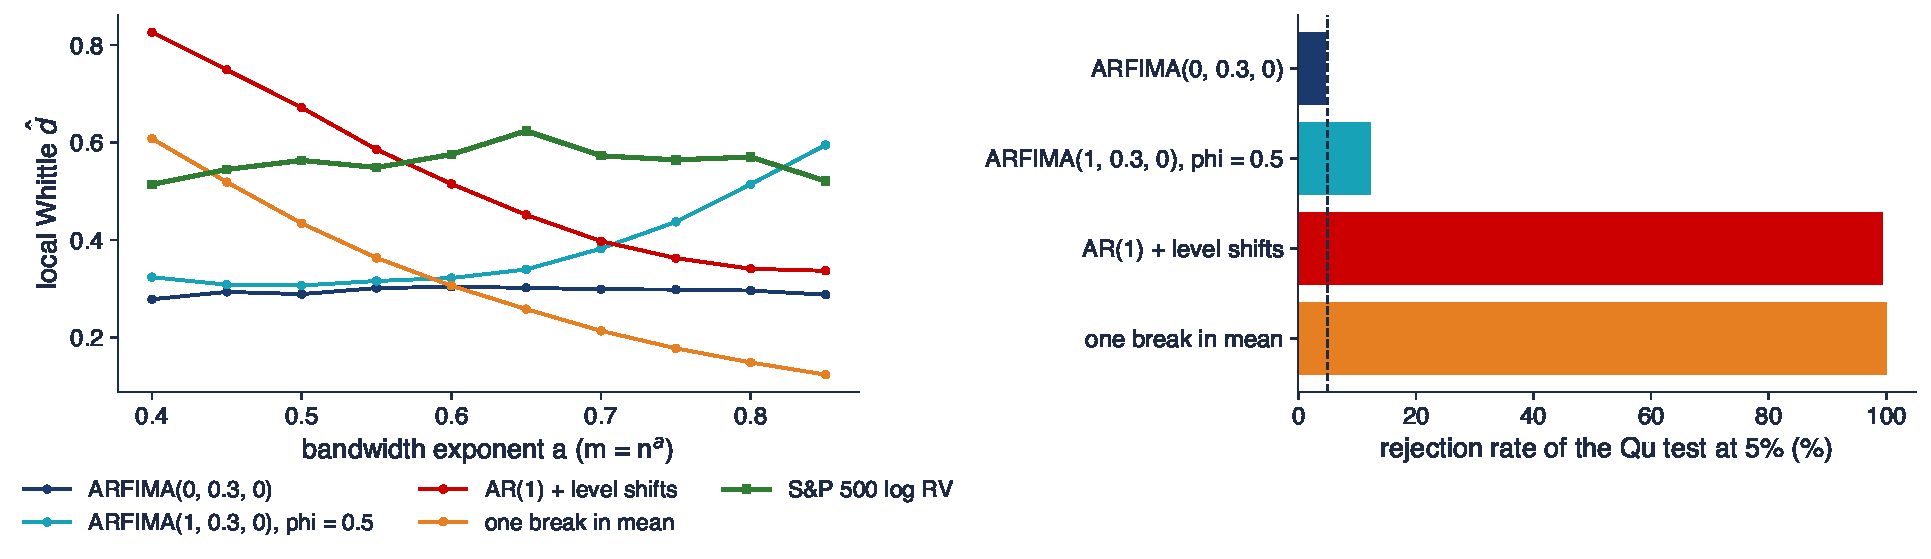
\includegraphics[width=0.97\textwidth,height=0.5\textheight,keepaspectratio]{ats_ch10_qu.pdf}
\end{center}
\vspace{-0.25cm}
\begin{itemize}
    \item $n = 2000$, 300 de replicări, $m = n^{0{,}7} = 204$, $\varepsilon = 0{,}02$; stînga: media $\hat d(m)$ local Whittle (100 de traiectorii) și logaritmul RV pentru S\&P 500; dreapta: ratele de respingere la 5\%
\end{itemize}
\quantlet{ATS\_ch10\_qu\_test}{\qlurl{ATS_ch10_qu_test}}
\end{frame}

\begin{frame}{Interpretarea testului Qu}
\itemsize{\small}
\begin{itemize}
    \item Mărimea: 5\% sub ARFIMA$(0; 0{,}3; 0)$, 12\% cînd se adaugă un AR(1) cu $\phi = 0{,}5$: dinamica de termen scurt distorsionează mărimea în eșantioane finite
    \item Puterea: 99\% împotriva salturilor de nivel și 100\% împotriva unei singure rupturi, deși LW raportează $\hat d = 0{,}39$ și 0{,}21
    \item Semnătura: sub salturi de nivel, $\hat d(m)$ scade de la 0{,}83 la 0{,}34; logaritmul RV pentru S\&P 500 rămîne între 0{,}51 și 0{,}62, iar $W = 0{,}66$ este mult sub valoarea de 10\%
    \item Memoria varianței realizate trece acest test; secțiunea 5 arată că $|r_t|$ pentru BET și EUR/RON nu îl trece
\end{itemize}
\end{frame}

\begin{frame}{Persistența inflației și dezinflația}
\itemsize{\footnotesize}
\begin{center}
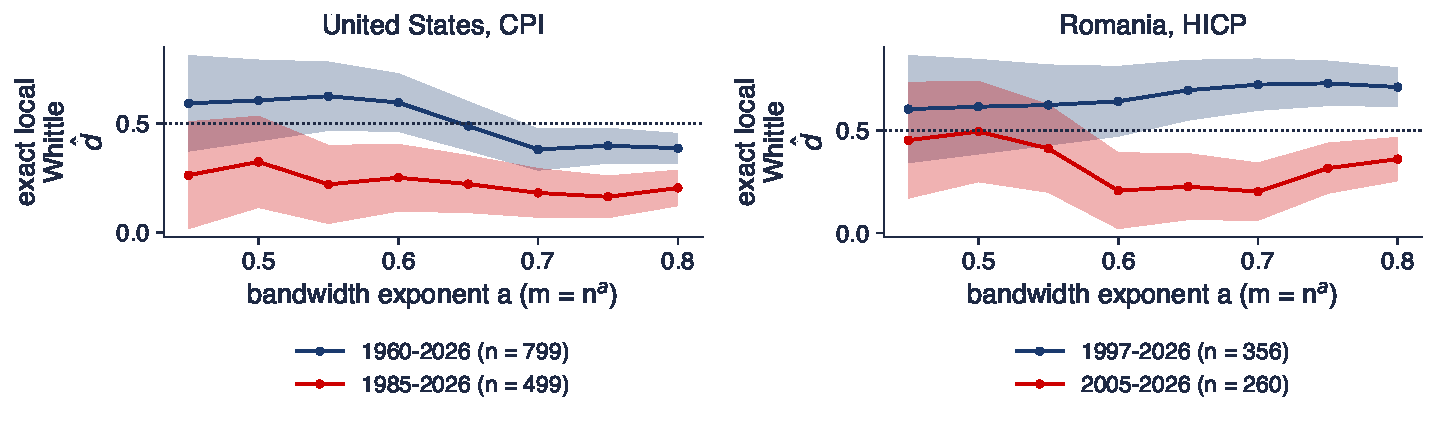
\includegraphics[width=0.97\textwidth,height=0.5\textheight,keepaspectratio]{ats_ch10_inflation.pdf}
\end{center}
\vspace{-0.25cm}
\begin{itemize}
    \item Inflația lunară, \% anualizat: IPC SUA (ajustat sezonier) pînă în august 2026, IAPC România (fără mediile lunare) pînă în august 2026; local Whittle exact cu media necunoscută, benzi de 95\%; eșantionul complet și după dezinflație (SUA din 1985, România din 2005)
\end{itemize}
\quantlet{ATS\_ch10\_qu\_test}{\qlurl{ATS_ch10_qu_test}}
\end{frame}

\begin{frame}{Interpretarea persistenței inflației}
\itemsize{\small}
\begin{itemize}
    \item SUA: $\hat d = 0{,}49$ (SE 0{,}06) pe 1960--2026, dar 0{,}22 după 1985; Qu $W = 1{,}62$ (valoarea de 1\%: 1{,}45) respinge pentru eșantionul complet, $W = 0{,}55$ după 1985
    \item România: $\hat d = 0{,}70$ cu dezinflația din 1997--2004, 0{,}23 din 2005 (între 0{,}20 și 0{,}50 după lățimea de bandă); $W = 0{,}86$ și 1{,}04, cu doar 356 și 260 de luni
    \item Local Whittle simplu pe eșantionul complet pentru România dă 0{,}31: cu un salt de nivel asemănător unui trend, doar versiunea exactă cu media Shimotsu este de încredere
    \item În interiorul unui regim monetar stabil, inflația păstrează o memorie lungă moderată, $\hat d$ = 0{,}22 și 0{,}23 \refHW, \refBCT; estimațiile mari aparțin schimbărilor de regim
\end{itemize}
\end{frame}

\begin{frame}{Recapitulare: memorie scurtă sau lungă}
\itemsize{\small}
\begin{itemize}
    \item Rupturile, salturile de nivel și schimbările rare de regim creează un pol spectral și un $\hat d$ mare
    \item Diagnostic: $\hat d(m)$ scade cu $m$; test: Qu (2011), cu valori critice simulate
    \item Inflația din SUA: memoria lungă provine în mare parte din Marea Inflație; logaritmul RV trece testul
\end{itemize}
\end{frame}


%=============================================================================
\section{Cointegrarea fracționară}
%=============================================================================

\begin{frame}{Cointegrarea fracționară și FCVAR (1/2)}
\itemsize{\small}
\begin{itemize}
    \item $X_t \in \mathbb R^p$ este I($d$); este \textbf{cointegrat fracționar} dacă $\beta'X_t$ este I($d - b$), $b > 0$
    \begin{itemize}
        \item $d$: memoria seriilor; $b$: reducerea memoriei obținută prin combinația $\beta'X_t$; \atschlink{https://danpele.github.io/Advanced-Time-Series/RO/Cursuri/capitol4_cointegrare_vecm_ardl_panel.pdf}{Capitolul 4} este cazul $d = b = 1$
    \end{itemize}
    \item FCVAR \refJN: VECM în care diferența $\Delta$ este înlocuită cu diferențe fracționare
    \[ \Delta^dX_t = \alpha\beta'L_b\Delta^{d-b}X_t + \sum_{i=1}^k\Gamma_i\Delta^dL_b^iX_t + \varepsilon_t, \qquad L_b = 1 - \Delta^b \]
    \begin{itemize}
        \item $\Delta^d = (1 - L)^d$; $L_b$: operatorul lag fracționar ($L_1 = L$), deci $d = b = 1$ dă VECM
        \item $\alpha$ ($p \times r$): ajustarea; $\beta$ ($p \times r$): vectorii de cointegrare, rangul $r$; $\Gamma_i$: matricele de termen scurt, $k$ laguri; $\varepsilon_t$: erori i.i.d.
    \end{itemize}
\end{itemize}
\end{frame}

\begin{frame}{Cointegrarea fracționară și FCVAR (2/2): estimare și rang}
\itemsize{\small}
\begin{itemize}
    \item Pentru $(d, b)$ fixat: o regresie de rang redus a lui $Z_0 = \Delta^dX$ pe $Z_1 = L_b\Delta^{d-b}X$; apoi profilăm verosimilitatea în $(d, b)$
    \[ \ell_r(d, b) = -\frac T2\Big[\log\det S_{00} + \sum_{i\le r}\log(1 - \hat\lambda_i)\Big] \]
    \begin{itemize}
        \item $S_{00}$: covarianța reziduală a lui $Z_0$ (după termenii de termen scurt); $\hat\lambda_i$: valorile proprii Johansen, în ordine descrescătoare; $T$: mărimea eșantionului
    \end{itemize}
    \item Testele de rang: statistica trace LR pentru rangul $r$ față de $p$
    \begin{itemize}
        \item pentru $b < 1/2$ este asimptotic $\chi^2_{(p-r)^2}$; pentru $b > 1/2$ se folosesc distribuțiile Dickey--Fuller fracționare din \refMN
    \end{itemize}
\end{itemize}
\end{frame}

\begin{frame}{Memorie comună semiparametrică}
\itemsize{\small}
\begin{itemize}
    \item Cele mai mici pătrate în bandă îngustă (NBLS) \refRobA, \refCN: regresăm $y$ pe $x$ folosind doar cele mai joase $m$ frecvențe
    \[ \hat\beta = \frac{\mathrm{Re}\sum_{j=1}^mI_{xy}(\lambda_j)}{\sum_{j=1}^mI_{xx}(\lambda_j)} \]
    \begin{itemize}
        \item $I_{xy}$: periodograma încrucișată a lui $x$ și $y$; $I_{xx}$: periodograma lui $x$; $\mathrm{Re}$: partea reală
        \item doar frecvențele joase, acolo unde se află componenta comună cu memorie lungă: robust la corelația de termen scurt dintre $x$ și eroare, care deplasează OLS
    \end{itemize}
    \item Rangul prin ELW \refNS: estimăm $d$ pentru fiecare serie, testăm egalitatea lui $d$, apoi numărăm valorile proprii mici ale matricei spectrale de frecvență joasă
    \item Varianța implicită și cea realizată \refBP: conține VIX componenta cu memorie lungă a varianței realizate viitoare?
    \begin{itemize}
        \item dacă $\log RV$ și $\log VIX^2$ au un trend fracționar comun, o combinație are $d$ mai mic, iar VIX prognozează partea persistentă
    \end{itemize}
\end{itemize}
\end{frame}

\begin{frame}{FCVAR: varianța realizată și cea implicită}
\itemsize{\footnotesize}
\begin{center}
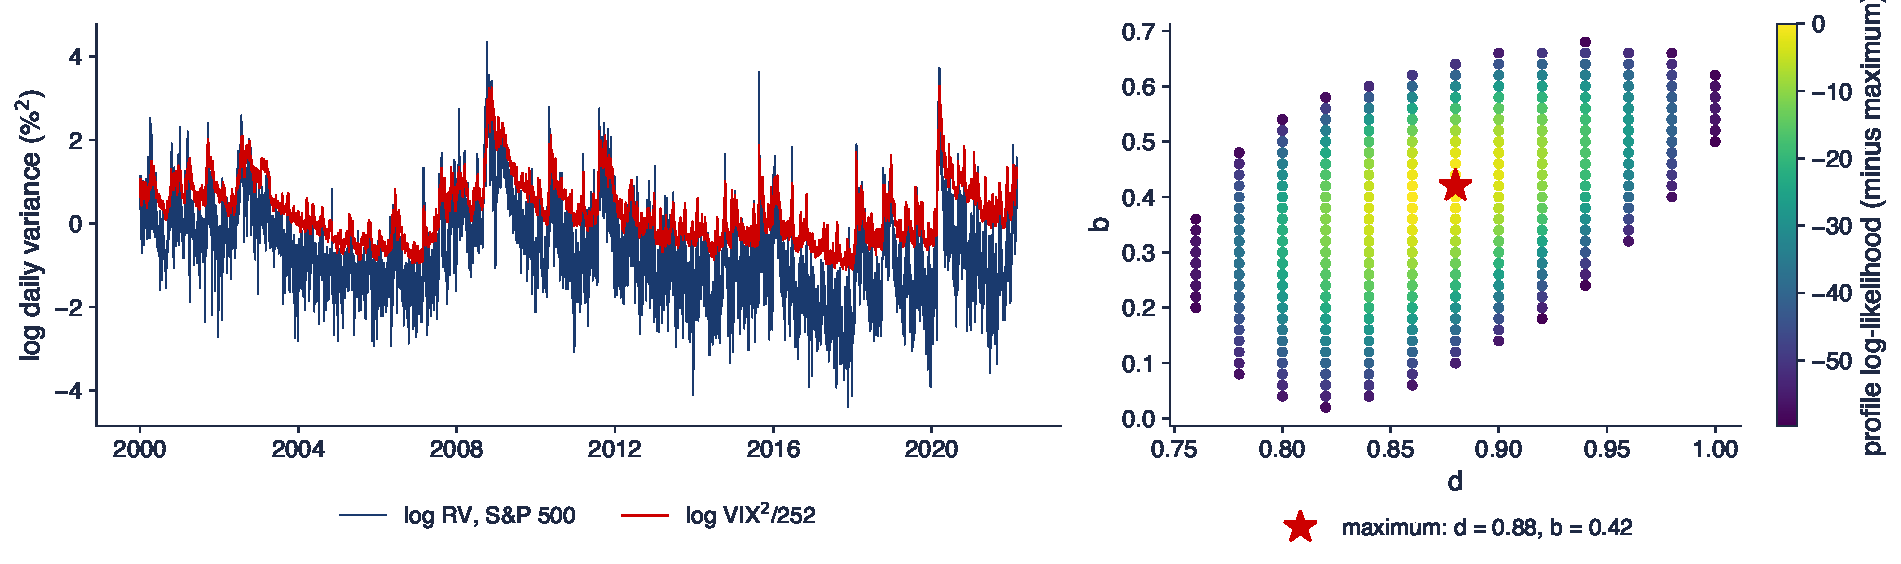
\includegraphics[width=0.97\textwidth,height=0.48\textheight,keepaspectratio]{ats_ch10_fcvar.pdf}
\end{center}
\vspace{-0.25cm}
\begin{itemize}
    \item Logaritmul RV de 5 minute pentru S\&P 500 și $\log(\mathrm{VIX}^2/252)$, $n = 5\,523$ zile comune pînă la 25 februarie 2022; dreapta: log-verosimilitatea profilată a FCVAR de rang unu cu $k = 0$ în $(d, b)$, ultimele 60 de puncte logaritmice sub maxim
\end{itemize}
\quantlet{ATS\_ch10\_fcvar}{\qlurl{ATS_ch10_fcvar}}
\end{frame}

\begin{frame}{Interpretarea modelului FCVAR}
\itemsize{\small}
\begin{itemize}
    \item Local Whittle: $d$ = 0{,}62 pentru logaritmul RV, 0{,}83 pentru logaritmul VIX$^2$, 0{,}49 pentru combinația $\beta'X_t$ (SE 0{,}03): combinația este mai puțin persistentă
    \item FCVAR: $\hat d = 0{,}88$, $\hat b = 0{,}42$, $\beta = (1; -1{,}70)$, $\alpha = (\ensuremath{-}1{,}55; 0{,}006)$: varianța realizată se ajustează, VIX nu (exogenitate slabă)
    \item Testele trace ($\hat b < 1/2$, deci $\chi^2$): rangul 0 față de 2: 1453{,}94 ($p$ $<$0{,}001); rangul 1 față de 2: 18{,}26 ($p$ $<$0{,}001): cu $k = 0$ datele resping și ipoteza unei singure relații
    \item Panta NBLS a logaritmului RV pe logaritmul VIX$^2$: 1{,}27, față de $1/1{,}70 = 0{,}59$ implicată de FCVAR: dinamica de termen scurt ($k > 0$) și intervalul overnight al RV lipsesc; o întrebare de proiect
\end{itemize}
\end{frame}

\begin{frame}{Recapitulare: cointegrarea fracționară}
\itemsize{\small}
\begin{itemize}
    \item FCVAR generalizează VECM cu doi parametri de memorie, $d$ și $b$, estimați prin verosimilitate profilată și regresie de rang redus
    \item Testele de rang sînt $\chi^2$ doar pentru $b < 1/2$; NBLS și ELW dau verificări semiparametrice
    \item Varianța realizată și cea implicită au componente persistente comune; structura exactă cere dinamica de termen scurt
\end{itemize}
\end{frame}


%=============================================================================
\section{Memoria lungă a volatilității}
%=============================================================================

\begin{frame}{FIGARCH (1/2): ponderi ARCH hiperbolice}
\itemsize{\small}
\begin{itemize}
    \item GARCH(1,1) ca ARCH($\infty$): ponderile pătratelor șocurilor trecute scad geometric
    \[ \sigma_t^2 = \frac{\omega}{1 - \beta} + \sum_{k\ge1}\alpha\beta^{k-1}\varepsilon_{t-k}^2 \]
    \item FIGARCH(1,$d$,1) \refBBM: o diferență fracționară le face să scadă hiperbolic
    \[ \sigma_t^2 = \frac{\omega}{1 - \beta} + \Big[1 - \frac{(1 - \phi L)(1 - L)^d}{1 - \beta L}\Big]\varepsilon_t^2 = \frac{\omega}{1 - \beta} + \sum_{k\ge1}\lambda_k\varepsilon_{t-k}^2 \]
    \begin{itemize}
        \item $d \in (0, 1)$: memoria volatilității; $\phi$, $\beta$: termenii ARCH și GARCH de termen scurt; $\lambda_k \sim c\,k^{-d-1}$: ponderile ARCH($\infty$)
        \item pozitivitatea tuturor $\lambda_k$ cere restricții, de exemplu $\beta - d \le \phi \le (2 - d)/3$
    \end{itemize}
\end{itemize}
\end{frame}

\begin{frame}{FIGARCH (2/2): paradoxul varianței și HYGARCH}
\itemsize{\small}
\begin{itemize}
    \item Paradoxul: $\sum_k\lambda_k = 1$, deci $\E\varepsilon_t^2 = \infty$
    \begin{itemize}
        \item FIGARCH nu este staționar în covarianță pentru niciun $d > 0$, deși este strict staționar
        \item memoria lungă a lui $\varepsilon_t^2$ nu este deci definită printr-o autocovarianță
    \end{itemize}
    \item HYGARCH \refDav: $(1 - L)^d$ este înlocuit cu $1 + a\big((1 - L)^d - 1\big)$
    \begin{itemize}
        \item $a \ge 0$: amplitudinea părții hiperbolice; $a < 1$ dă o varianță finită și memorie hiperbolică, $a = 1$ este FIGARCH, $a = 0$ este GARCH
    \end{itemize}
\end{itemize}
\end{frame}

\begin{frame}{Ponderi ARCH: geometrice și hiperbolice}
\itemsize{\footnotesize}
\begin{center}
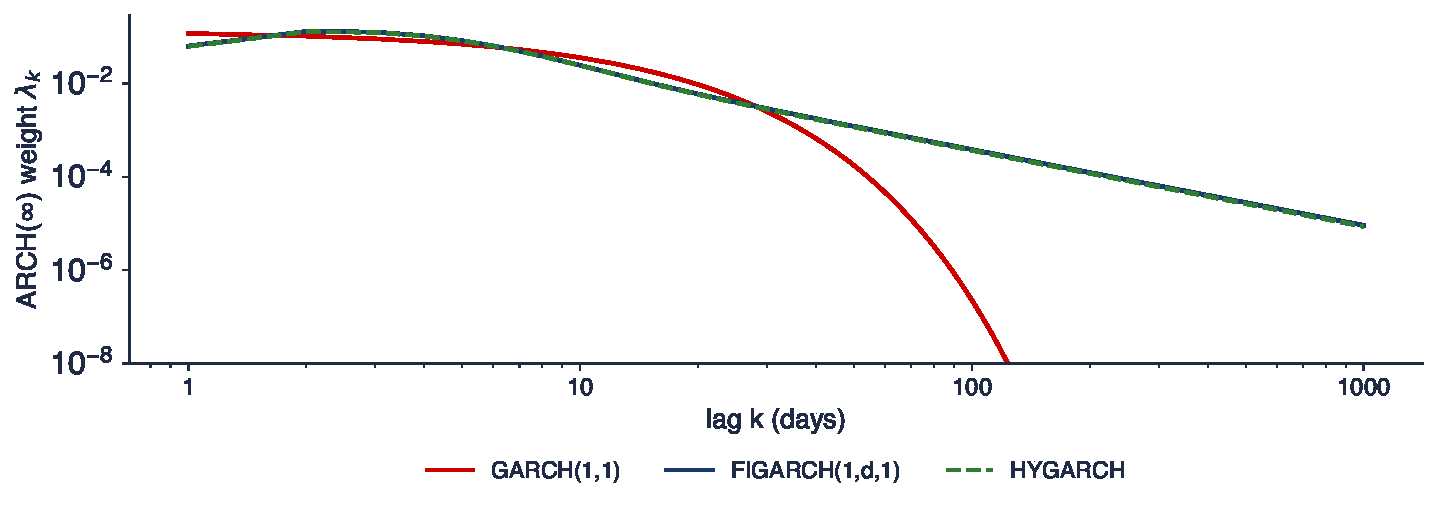
\includegraphics[width=0.97\textwidth,height=0.48\textheight,keepaspectratio]{ats_ch10_figarch.pdf}
\end{center}
\vspace{-0.25cm}
\begin{itemize}
    \item Randamentele zilnice ale S\&P 500, 2000--2026 ($n = 6\,714$), QML cu distribuția Student $t$, ARCH($\infty$) trunchiat la 1000 de laguri; GARCH $(\alpha, \beta) = (0{,}119; 0{,}876)$, FIGARCH $d = 0{,}61$, $\phi = 0{,}04$, $\beta = 0{,}59$
\end{itemize}
\quantlet{ATS\_ch10\_figarch}{\qlurl{ATS_ch10_figarch}}
\end{frame}

\begin{frame}{Interpretarea estimațiilor FIGARCH}
\itemsize{\footnotesize}
\begin{center}
\scriptsize
\begin{tabular}{lcccccc}
\toprule
\textbf{Piața} & $\hat d$ & LR & $\hat a$ & BIC GARCH & BIC FIGARCH & ponderea după lagul 22 \\
\midrule
S\&P 500 & 0{,}61 & 40{,}8 & 0{,}99 & 18197 & 18165 & 15\% / 5\% \\
BET & 0{,}46 & 79{,}0 & 1{,}00 & 19514 & 19444 & 17\% / 1\% \\
Bitcoin & 0{,}98 & 13{,}6 & 1{,}06 & 20942 & 20936 & 12\% / 8\% \\
\bottomrule
\end{tabular}
\end{center}
\begin{itemize}
    \item LR pentru FIGARCH față de GARCH (un parametru în plus): 40{,}8; 79{,}0; 13{,}6; BIC preferă FIGARCH pe toate cele trei piețe
    \item Ponderea șocurilor pătratice mai vechi de 22 de zile: FIGARCH 15\%, GARCH 5\% (S\&P 500); după 250 de zile 2{,}0\% față de practic zero
    \item Amplitudinea HYGARCH $\hat a$ = 0{,}99 și 1{,}00: nicio evidență împotriva lui $a = 1$ (LR 0{,}22 și 0{,}01); pentru Bitcoin $\hat d = 0{,}98$ se află la marginea integrată
    \item LR: statistica raportului de verosimilitate pentru FIGARCH față de GARCH; $\hat a$: amplitudinea HYGARCH; ultima coloană: FIGARCH / GARCH
\end{itemize}
\end{frame}

\begin{frame}{Volatilitate stochastică cu memorie lungă și zgomot}
\itemsize{\small}
\begin{itemize}
    \item LMSV \refBCL: logaritmul varianței este un proces cu memorie lungă; ridicarea la pătrat și logaritmarea fac modelul liniar
    \[ r_t = \sigma_t\eta_t, \quad \log\sigma_t^2 = \mu + h_t \ \Rightarrow\ \log r_t^2 = \mu + \E\log\eta^2 + h_t + \xi_t \]
    \begin{itemize}
        \item $h_t$: ARFIMA$(p,d,q)$; $\eta_t$: șoc i.i.d.; $\xi_t = \log\eta_t^2 - \E\log\eta^2$: zgomot i.i.d.\ cu varianța $\pi^2/2$ pentru $\eta$ gaussian, adesea mai mare decît $\Var(h_t)$
    \end{itemize}
    \item Spectrul lui $\log r_t^2$: un pol plus un nivel plat al zgomotului
    \[ f(\lambda) = G\lambda^{-2d} + \frac{\sigma_\xi^2}{2\pi} \]
    \begin{itemize}
        \item zgomotul plat aplatizează panta de frecvență joasă și deplasează $\hat d$ în jos
        \item LW cu zgomot \refHMS: $f(\lambda) = G(\lambda^{-2d} + \theta)$, cu raportul zgomot/semnal $\theta \ge 0$ estimat simultan; consistent, cu o viteză mai mică
    \end{itemize}
    \item Varianța realizată reduce zgomotul prin medierea randamentelor intraday \refABDL: $\log RV_t = \log IV_t + $ o eroare mică
    \item Memoria lungă a volatilității în timp continuu: \refCR; alternativa rough volatility urmează în secțiunea 6
\end{itemize}
\end{frame}

\begin{frame}{Memoria proxy-urilor de volatilitate pe mai multe piețe}
\itemsize{\footnotesize}
\begin{center}
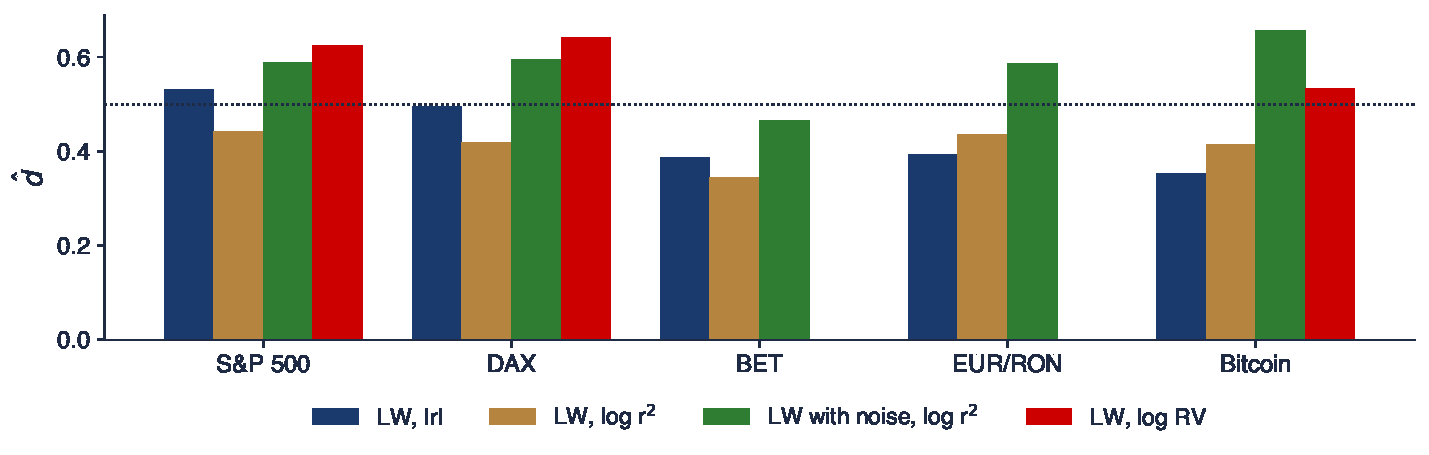
\includegraphics[width=0.97\textwidth,height=0.5\textheight,keepaspectratio]{ats_ch10_assets_d.pdf}
\end{center}
\vspace{-0.25cm}
\begin{itemize}
    \item $\hat d$ local Whittle cu $m = n^{0{,}65}$ pentru $|r_t|$ și $\log(r_t^2 + c)$, $c$ = 1\% din varianță; LW cu zgomot pentru $\log(r_t^2 + c)$ cu $m = n^{0{,}8}$; logaritmul RV acolo unde există măsuri realizate (S\&P 500, DAX pînă în 2022; Bitcoin pînă în 2026)
\end{itemize}
\quantlet{ATS\_ch10\_figarch}{\qlurl{ATS_ch10_figarch}}
\end{frame}

\begin{frame}{Interpretarea memoriei volatilității pe mai multe piețe}
\itemsize{\small}
\begin{itemize}
    \item S\&P 500: $|r|$ 0{,}53, $\log r^2$ 0{,}44, cu zgomot 0{,}59, logaritmul RV 0{,}62: corecția de zgomot aduce $\log r^2$ la nivelul RV
    \item Bitcoin: $\log r^2$ 0{,}41, cu zgomot 0{,}66, logaritmul RV 0{,}53; DAX: 0{,}42; 0{,}59; 0{,}64
    \item Testul Qu pe $|r_t|$ (valoarea de 1\%: 1{,}56): S\&P 500 0{,}78, DAX 0{,}72, Bitcoin 0{,}79; BET 1{,}71 și EUR/RON 1{,}88 resping
    \item Pentru BET și leu, o parte a memoriei aparente vine din schimbări de regim (2008, regimul de managed float): modelați întîi rupturile (\atschlink{https://danpele.github.io/Advanced-Time-Series/RO/Cursuri/capitol2_rupturi_structurale_modele_neliniare.pdf}{Capitolul 2})
\end{itemize}
\end{frame}

\begin{frame}{HAR ca aproximare a memoriei lungi}
\itemsize{\small}
\begin{itemize}
    \item HAR \refCor\ pentru $y = \log RV$ (\atschlink{https://danpele.github.io/Advanced-Time-Series/RO/Cursuri/capitol8_volatilitate_avansata.pdf}{Capitolul 8})
    \[ y_{t+1} = \beta_0 + \beta_dy_t + \beta_w\bar y_t^{(5)} + \beta_m\bar y_t^{(22)} + u_{t+1} \]
    \begin{itemize}
        \item $\bar y_t^{(5)}$, $\bar y_t^{(22)}$: mediile lui $y$ pe ultimele 5 și 22 de zile; un AR(22) cu trei pante libere: o aproximare în trepte a ponderilor AR cu descreștere hiperbolică
    \end{itemize}
    \item Formal, memorie scurtă: ACF scade geometric, dar pe orizonturi de pînă la cîteva luni imită $k^{2d-1}$
    \begin{itemize}
        \item interpretarea în cascadă: participanți cu orizonturi zilnice, săptămînale și lunare (ipoteza pieței eterogene)
    \end{itemize}
    \item Estimat prin OLS, ușor de extins (salturi, semivarianțe, \atschlink{https://danpele.github.io/Advanced-Time-Series/RO/Cursuri/capitol8_volatilitate_avansata.pdf}{Capitolul 8}): reperul pe care orice model cu memorie lungă sau de tip rough volatility trebuie să îl depășească
\end{itemize}
\end{frame}

\begin{frame}{Ponderile HAR și ACF implicată}
\itemsize{\footnotesize}
\begin{center}
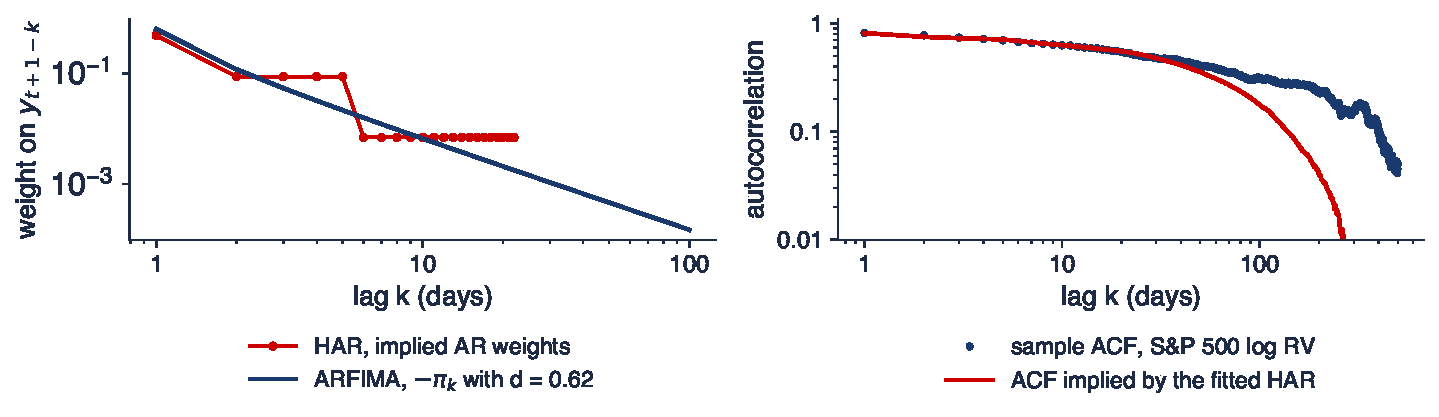
\includegraphics[width=0.97\textwidth,height=0.48\textheight,keepaspectratio]{ats_ch10_har_approx.pdf}
\end{center}
\vspace{-0.25cm}
\begin{itemize}
    \item Logaritmul RV pentru S\&P 500; HAR prin OLS: $\beta_d = 0{,}39$, $\beta_w = 0{,}40$, $\beta_m = 0{,}15$; stînga: ponderile AR implicate și $-\pi_k$ ARFIMA cu $d = 0{,}62$; dreapta: ACF a unei simulări lungi a HAR estimat și ACF de eșantion
\end{itemize}
\quantlet{ATS\_ch10\_figarch}{\qlurl{ATS_ch10_figarch}}
\end{frame}

\begin{frame}{Interpretarea aproximării HAR}
\itemsize{\small}
\begin{itemize}
    \item Suma ponderilor HAR 0{,}946: aproape de o rădăcină unitară, așa își obține persistența un model de memorie scurtă
    \item ACF la lagul 100: eșantion 0{,}31, HAR 0{,}179; la 250: 0{,}18 față de 0{,}017
    \item ACF implicată scade sub jumătatea ACF de eșantion după lagul 112: HAR captează memoria pînă la circa o jumătate de an
    \item Pentru prognoze de pînă la o lună aceasta ajunge, de aceea HAR este greu de depășit (secțiunea 7)
\end{itemize}
\end{frame}

\begin{frame}{Recapitulare: memoria lungă a volatilității}
\itemsize{\small}
\begin{itemize}
    \item FIGARCH are ponderi ARCH hiperbolice, dar varianță infinită; HYGARCH îl include
    \item $\log r_t^2$ este memorie lungă plus zgomot mare: folosiți LW robust la zgomot sau măsurile realizate
    \item HAR este un model cu memorie scurtă care imită memoria lungă pe orizonturile relevante pentru prognoză
\end{itemize}
\end{frame}


%=============================================================================
\section{Rough volatility}
%=============================================================================

\begin{frame}{Mișcarea browniană fracționară (1/2)}
\itemsize{\footnotesize}
\begin{columns}[T]
\begin{column}{0.32\textwidth}
\centering
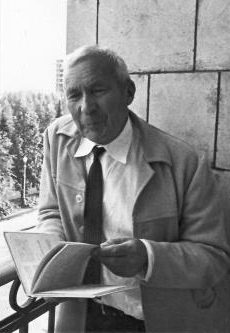
\includegraphics[height=0.25\textheight]{ch10_kolmogorov.jpg}\\[1mm]
\imgcap{A. N. Kolmogorov}
\imgcredit{https://commons.wikimedia.org/wiki/File:Andrej_Nikolajewitsch_Kolmogorov.jpg}{Foto: Konrad Jacobs; CC BY-SA 2.0 de; Wikimedia Commons}\\[1mm]\centering
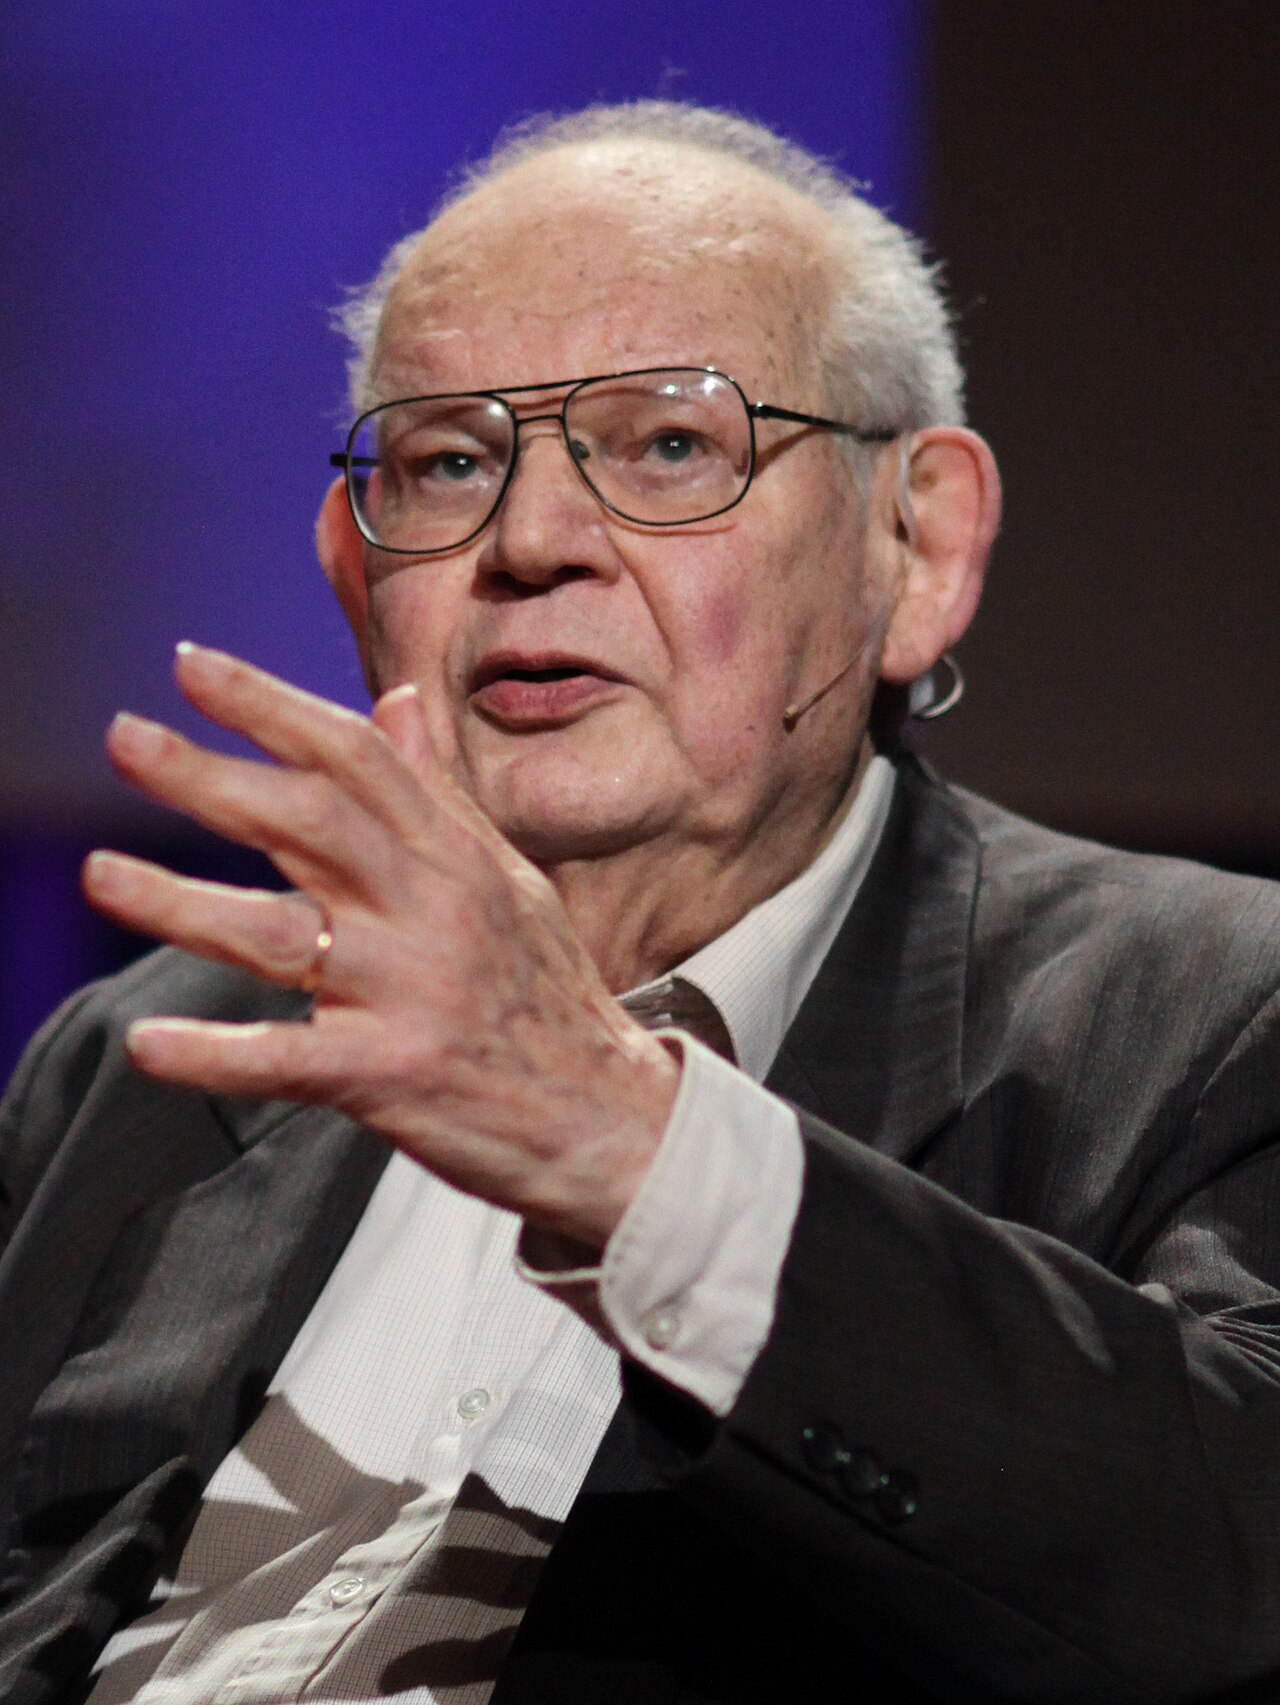
\includegraphics[height=0.15\textheight]{ch10_mandelbrot_2010.jpg}\\[1mm]
\imgcap{B. B. Mandelbrot, TED 2010}
\imgcredit{https://commons.wikimedia.org/wiki/File:Benoit_Mandelbrot,_TED_2010_(3x4_cropped).jpg}{Foto: Steve Jurvetson (2010); CC BY 2.0; Wikimedia Commons}
\end{column}
\begin{column}{0.66\textwidth}
\begin{itemize}
    \item fBm $W^H_t$ \refMVN: un proces gaussian centrat, cu $W^H_0 = 0$ și covarianța
    \[ \E W^H_tW^H_s = \frac12\big(t^{2H} + s^{2H} - |t - s|^{2H}\big), \qquad H \in (0, 1) \]
    \begin{itemize}
        \item $H$: exponentul Hurst; $H = 1/2$ dă mișcarea browniană standard
        \item creșteri staționare, cu $\E|W^H_{t+\Delta} - W^H_t|^2 = \Delta^{2H}$
        \item autosimilar: $W^H_{ct} \overset{d}{=} c^HW^H_t$ (egalitate în distribuție) pentru $c > 0$
    \end{itemize}
\end{itemize}
\end{column}
\end{columns}
\end{frame}

\begin{frame}{Mișcarea browniană fracționară (2/2)}
\itemsize{\small}
\begin{itemize}
    \item Traiectoriile sînt continue Hölder de orice ordin $< H$
    \begin{itemize}
        \item ordinul Hölder: cît de repede poate scădea $|W^H_{t+\Delta} - W^H_t|$ cu $\Delta$; $H < 1/2$: traiectorii mai neregulate, $H > 1/2$: mai netede decît mișcarea browniană
    \end{itemize}
    \item Creșterile, zgomotul gaussian fracționar (fGn), au autocorelațiile
    \[ \rho(k) = \frac12\big(|k + 1|^{2H} - 2|k|^{2H} + |k - 1|^{2H}\big) \sim H(2H - 1)k^{2H-2} \]
    \begin{itemize}
        \item memorie lungă pentru $H > 1/2$ ($d = H - 1/2$); corelație negativă pentru $H < 1/2$
    \end{itemize}
\end{itemize}
\end{frame}

\begin{frame}{Traiectorii browniene fracționare}
\itemsize{\footnotesize}
\begin{center}
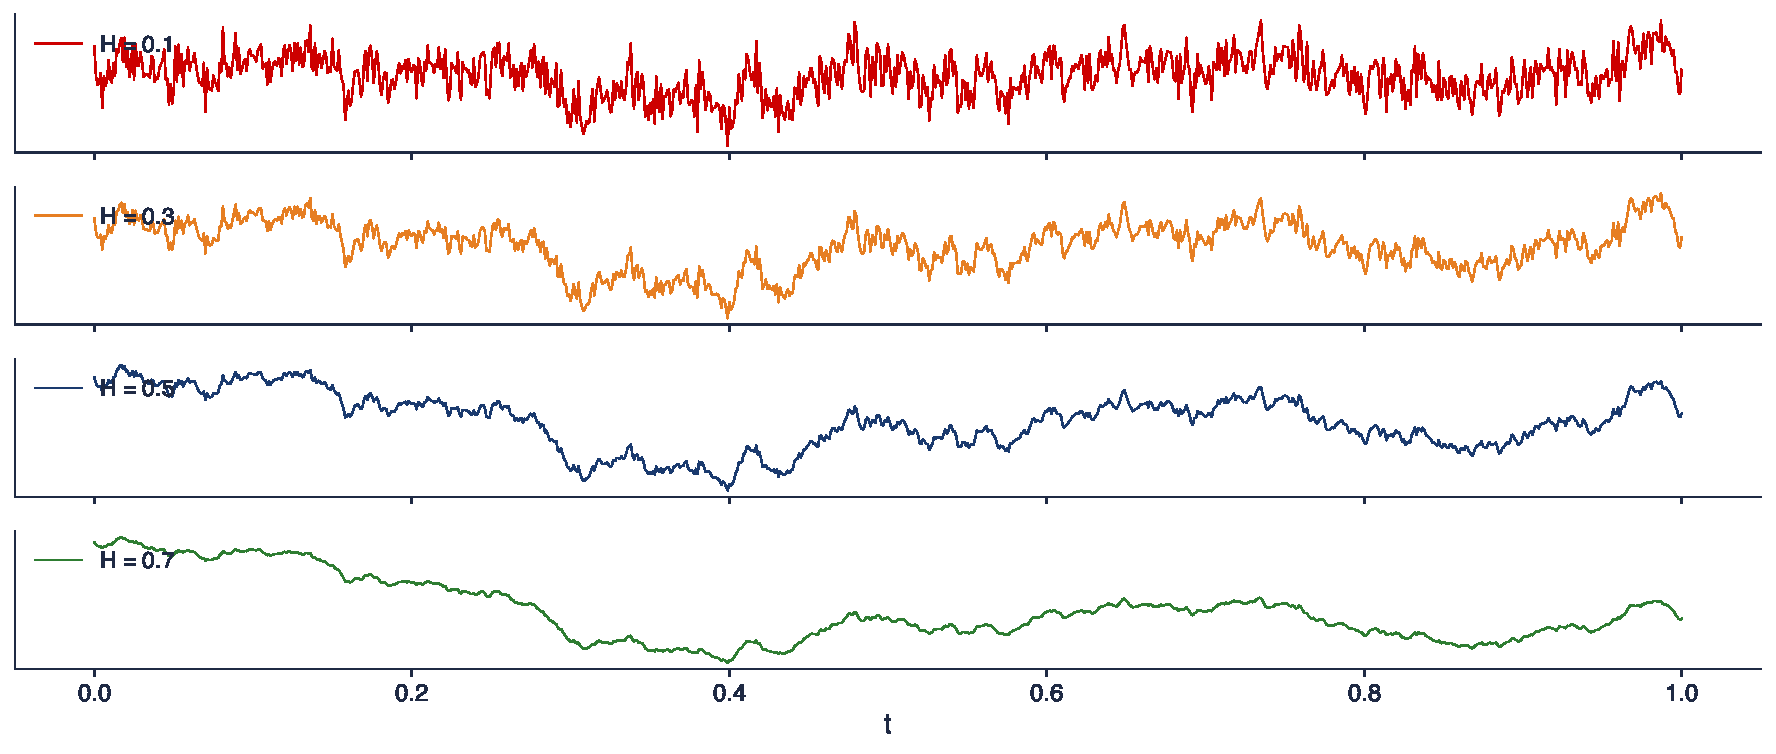
\includegraphics[width=0.97\textwidth,height=0.5\textheight,keepaspectratio]{ats_ch10_fbm_paths.pdf}
\end{center}
\vspace{-0.25cm}
\begin{itemize}
    \item O traiectorie pentru fiecare valoare, pe 1000 de pași, simulare exactă prin scufundare circulantă; $H = 0{,}5$ este mișcarea browniană
\end{itemize}
\quantlet{ATS\_ch10\_simulation}{\qlurl{ATS_ch10_simulation}}
\end{frame}

\begin{frame}{Interpretarea traiectoriilor}
\itemsize{\small}
\begin{itemize}
    \item Corelația de ordinul unu a creșterilor: \ensuremath{-}0{,}426 pentru $H = 0{,}1$, \ensuremath{-}0{,}242 pentru $H = 0{,}3$, 0 pentru $H = 0{,}5$, 0{,}320 pentru $H = 0{,}7$
    \item $H = 0{,}1$: fiecare creștere este probabil urmată de o scădere, deci traiectoria este zimțată la toate scările, dar se abate puțin
    \item $H = 0{,}7$: trendurile persistă; aceasta este lectura fBm a efectului Hurst
    \item Neregularitatea este o afirmație despre scările mici, persistența despre cele mari: păstrați-le separate
\end{itemize}
\end{frame}

\begin{frame}{Simularea fBm: Cholesky, scufundarea circulantă}
\itemsize{\small}
\begin{itemize}
    \item Cholesky: $\Gamma = LL'$, $X = LZ$; exact, dar cu timp $O(n^3)$ și memorie $O(n^2)$
    \begin{itemize}
        \item $\Gamma$: matricea de covarianță $n \times n$ a traiectoriei; $L$: factorul ei Cholesky inferior triunghiular; $Z$: un vector de variabile i.i.d. $N(0, 1)$
    \end{itemize}
    \item Davies--Harte \refDH, \refDN: scufundăm matricea Toeplitz $\Gamma$ a fGn într-o matrice circulantă de ordin $M = 2(n - 1)$, cu primul rînd $c = (\gamma_0, \dots, \gamma_{n-1}, \gamma_{n-2}, \dots, \gamma_1)$
    \begin{itemize}
        \item $\gamma_k$: autocovarianțele fGn; o matrice circulantă este diagonalizată de transformata Fourier discretă: valorile proprii $\Lambda = \mathrm{FFT}(c)$
        \item dacă $\Lambda \ge 0$: $Y = \mathrm{FFT}\big(\sqrt{\Lambda/M}\,(Z_1 + iZ_2)\big)$, cu $Z_1, Z_2$ vectori gaussieni standard independenți; $\mathrm{Re}\,Y$ și $\mathrm{Im}\,Y$ sînt două traiectorii exacte independente
    \end{itemize}
    \item $O(n\log n)$; pentru fGn $\Lambda \ge 0$ pentru orice $H$ (Seminarul 10, A7); fBm = fGn cumulat
    \item Același algoritm simulează exact ARFIMA$(0,d,0)$ (folosit în fiecare experiment Monte Carlo din acest capitol)
\end{itemize}
\end{frame}

\begin{frame}{Schema hibridă pentru procesele Volterra}
\itemsize{\footnotesize}
\begin{itemize}
    \item Modelele de rough volatility folosesc procese Volterra, nu fBm cu creșteri staționare \refBFG
    \[ X_t = \int_0^tg(t - s)\,dW_s, \qquad g(x) = x^{H-1/2} \ \ \text{(Riemann--Liouville)} \]
    \begin{itemize}
        \item $g$: nucleul, singular în 0 cînd $H < 1/2$; $W$: mișcarea browniană; scufundarea circulantă nu se aplică (proces nestaționar, posibil negaussian cînd este cuplat cu un preț corelat)
    \end{itemize}
    \item Schema hibridă \refBLPa: integrăm nucleul exact pe ultimul pas și folosim o sumă Riemann în puncte optime mai departe
    \[ X_i \approx \int_{t_{i-1}}^{t_i}(t_i - s)^{H-1/2}dW_s + \sum_{k\ge2}\Big(\frac{b_k}{n}\Big)^{H-1/2}\Delta W_{i-k+1} \]
    \[ b_k = \Big(\frac{k^{H+1/2} - (k - 1)^{H+1/2}}{H + 1/2}\Big)^{1/(H-1/2)} \]
    \begin{itemize}
        \item $n$: numărul de pași pe unitatea de timp; $\Delta W_i$: creșterile browniene; $b_k$: punctul optim de evaluare din celula $k$; primul termen și $\Delta W_i$ sînt gaussiene împreună și se simulează exact
    \end{itemize}
    \item Suma este o convoluție: $O(n\log n)$ prin FFT; schema se extinde la procesele browniene semistaționare
\end{itemize}
\end{frame}

\begin{frame}{Suma Riemann și schema hibridă}
\itemsize{\footnotesize}
\begin{center}
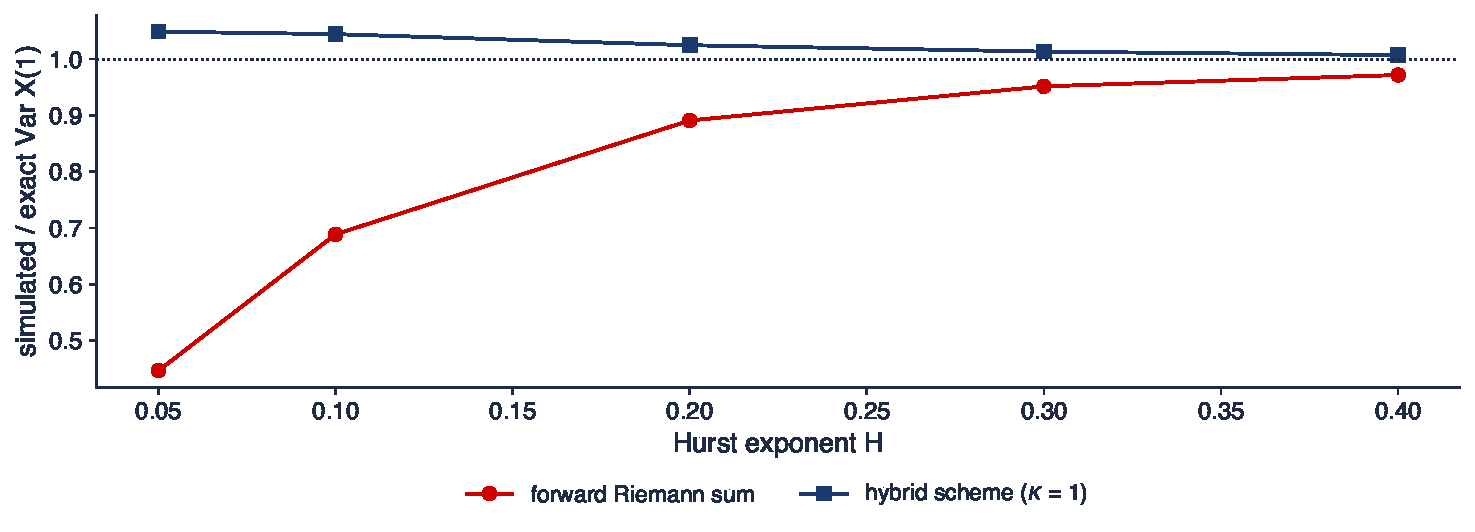
\includegraphics[width=0.97\textwidth,height=0.46\textheight,keepaspectratio]{ats_ch10_hybrid.pdf}
\end{center}
\vspace{-0.25cm}
\begin{itemize}
    \item $\Var X(1)$ pentru procesul Riemann--Liouville, valoarea exactă $1/(2H)$; $n = 250$ pași, 4\,000 de traiectorii
\end{itemize}
\quantlet{ATS\_ch10\_simulation}{\qlurl{ATS_ch10_simulation}}
\end{frame}

\begin{frame}{Interpretarea schemelor de simulare}
\itemsize{\small}
\begin{itemize}
    \item Suma Riemann înainte: 0{,}45 din varianța adevărată la $H = 0{,}05$ și 0{,}69 la $H = 0{,}1$: ratează masa nucleului de lîngă singularitate
    \item Schema hibridă: 1{,}05 și 1{,}04, în limita erorii Monte Carlo față de 1
    \item Eroarea schemei naive crește exact acolo unde se află rough volatility ($H \approx 0{,}1$): prețurile opțiunilor obținute cu ea ar fi deplasate
\end{itemize}
\end{frame}

\begin{frame}{Evidența: scalarea logaritmului volatilității (1/2)}
\itemsize{\small}
\begin{itemize}
    \item \refGJR, secțiunea 2: din $\sigma_t = \sqrt{RV_t}$ zilnic (biblioteca Oxford-Man), momentele empirice ale creșterilor lui $\log\sigma$
    \[ m(q, \Delta) = \frac1N\sum_t|\log\sigma_{t+\Delta} - \log\sigma_t|^q \]
    \begin{itemize}
        \item $\Delta$: lagul în zile; $q > 0$: ordinul momentului; $N$: numărul de perechi; $m(2, \Delta)$ este variograma
    \end{itemize}
    \item Dacă $\log\sigma$ are creșteri de tip fBm, momentele se scalează ca o putere a lui $\Delta$ (scalare monofractală)
    \[ m(q, \Delta) = K_q\nu^q\Delta^{\zeta_q}, \qquad \zeta_q = qH \]
    \begin{itemize}
        \item $\nu$: volatilitatea volatilității; $K_q = \E|Z|^q$, $Z \sim N(0, 1)$; $\zeta_q$: exponentul de scalare, liniar în $q$, cu panta $H$
        \item derivarea și abaterile de la această scalare: \atsapplink{atsapp2}{atssrc2}{Anexa}  % applink: scalarea momentelor fBm
    \end{itemize}
\end{itemize}
\end{frame}

\begin{frame}{Evidența: scalarea logaritmului volatilității (2/2)}
\itemsize{\small}
\begin{itemize}
    \item Procedura: OLS al lui $\log m(q, \Delta)$ pe $\log\Delta$ pentru fiecare $q$ dă $\zeta_q$; regresăm $\zeta_q$ pe $q$ prin origine pentru a obține $H$
    \begin{itemize}
        \item folosim $q \in \{0{,}5; 1; 1{,}5; 2; 3\}$ și $\Delta = 1, \dots, 50$ de zile
    \end{itemize}
    \item Rezultatul lor: $\zeta_q$ liniar și $H$ de ordinul 0,1 pentru toți indicii; creșterile logaritmului volatilității sînt apropiate de distribuția Normală
    \item Aceasta contrazice orice model SV markovian (Heston, log-OU), al cărui logaritm al volatilității are $H = 1/2$ la laguri scurte
\end{itemize}
\end{frame}

\begin{frame}{Replicarea scalării pe S\&P 500}
\itemsize{\footnotesize}
\begin{center}
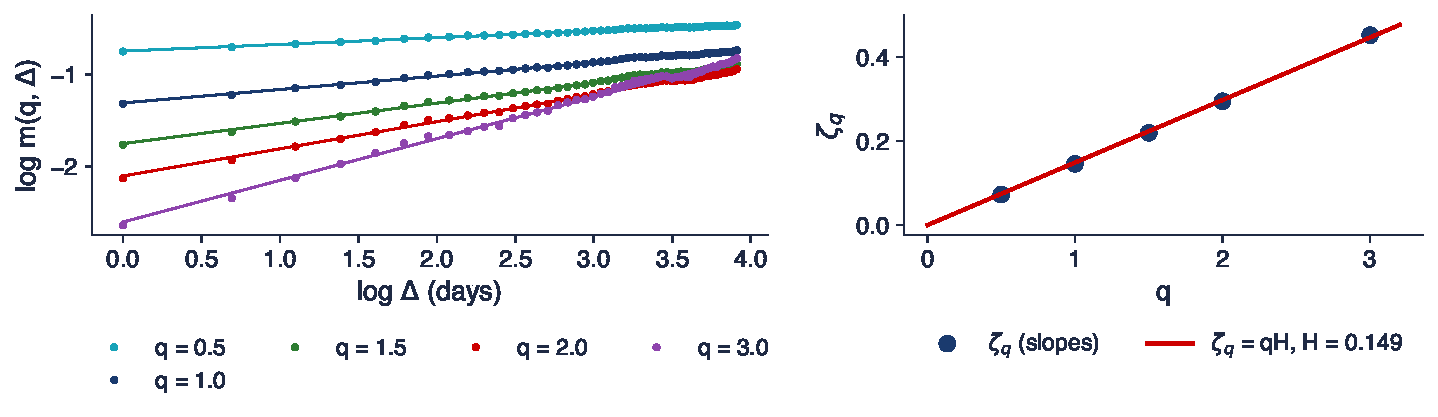
\includegraphics[width=0.97\textwidth,height=0.5\textheight,keepaspectratio]{ats_ch10_gjr.pdf}
\end{center}
\vspace{-0.25cm}
\begin{itemize}
    \item RV de 5 minute Oxford-Man pentru S\&P 500, ianuarie 2000 -- februarie 2022; stînga: $\log m(q, \Delta)$ și dreptele OLS; dreapta: $\zeta_q$ și dreapta $qH$
\end{itemize}
\quantlet{ATS\_ch10\_rough}{\qlurl{ATS_ch10_rough}}
\end{frame}

\begin{frame}{Interpretarea scalării}
\itemsize{\small}
\begin{itemize}
    \item $\zeta_q$ = 0{,}073; 0{,}146; 0{,}220; 0{,}295; 0{,}452 pentru $q$ = 0,5; 1; 1,5; 2; 3: liniar în $q$, $\hat H = 0{,}149$
    \item Volatilitatea volatilității $\hat\nu = 0{,}35$ din $m(2, \Delta) = \nu^2\Delta^{2H}$; subeșantioane: 0{,}140 (2000--2010), 0{,}155 (2011--2022)
    \item Rezultatul lucrării se replică: aproximativ $H \approx 0{,}1$--0,15, stabil în timp
    \item Legătura cu secțiunea 1: pe scara ARFIMA aceasta înseamnă $d = H + 1/2 \approx 0{,}65$, aproape de $\hat d$ local Whittle al logaritmului RV
\end{itemize}
\end{frame}

\begin{frame}{Modelul RFSV}
\itemsize{\small}
\begin{itemize}
    \item \refGJR: rough fractional stochastic volatility (RFSV), logaritmul volatilității este un proces Ornstein--Uhlenbeck (OU) fracționar
    \[ \sigma_t = \exp(X_t), \qquad dX_t = \nu\,dW^H_t - \alpha(X_t - m)\,dt, \qquad H < 1/2 \]
    \begin{itemize}
        \item $\nu$: volatilitatea volatilității; $m$: media de termen lung a lui $X$; $\alpha > 0$: viteza revenirii la medie, foarte mică
        \item pentru $\alpha T \ll 1$ ($T$: lungimea eșantionului) creșterile se comportă ca ale lui $\nu W^H$; staționaritatea apare doar pe orizonturi de ordinul $1/\alpha$
    \end{itemize}
    \item Legătura cu memoria lungă: pe orizonturile observabile, $\log\sigma$ este aproape de o fBm nestaționară cu $H \approx 0{,}1$, a cărei lectură ARFIMA este $d = H + 1/2 \approx 0{,}6$
    \begin{itemize}
        \item GJR arată că local Whittle și estimatori similari aplicați simulărilor RFSV dau valorile de „memorie lungă” găsite în literatură
    \end{itemize}
    \item Evaluarea opțiunilor: rough Bergomi \refBFG\ și rough Heston \refER
    \begin{itemize}
        \item ambele reproduc structura la termen a pantei volatilității implicite, $\propto \tau^{H-1/2}$ ($\tau$: scadența opțiunii), cu puțini parametri
        \item estimările din opțiuni dau tot $H$ mic \refLMPR
        \item partea de evaluare aparține MFM; aici testăm afirmația de serie de timp
    \end{itemize}
\end{itemize}
\end{frame}

\begin{frame}{Neregularitatea pe mai multe piețe și proxy-uri}
\itemsize{\footnotesize}
\begin{center}
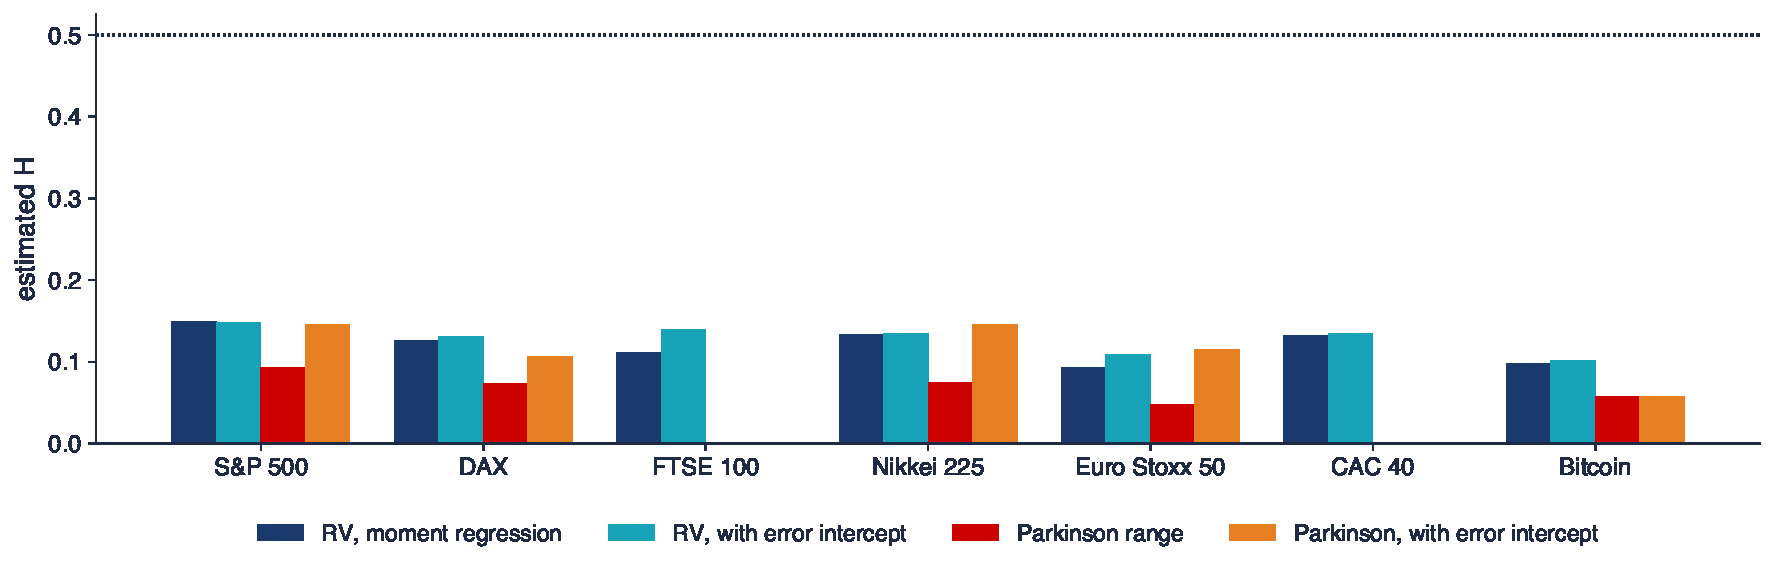
\includegraphics[width=0.97\textwidth,height=0.5\textheight,keepaspectratio]{ats_ch10_gjr_assets.pdf}
\end{center}
\vspace{-0.25cm}
\begin{itemize}
    \item $H$ din RV de 5 minute (Oxford-Man; Bitcoin: Binance) prin regresia momentelor și cu un termen liber pentru eroarea de măsurare; amplitudinea Parkinson din maximele și minimele zilnice EODHD pe aceleași zile, acolo unde există
\end{itemize}
\quantlet{ATS\_ch10\_rough}{\qlurl{ATS_ch10_rough}}
\end{frame}

\begin{frame}{Interpretarea neregularității pe mai multe piețe}
\itemsize{\small}
\begin{itemize}
    \item RV: $H$ între 0{,}09 și 0{,}15 pentru șase indici și Bitcoin (S\&P 500 0{,}15, DAX 0{,}13, Euro Stoxx 50 0{,}09, Bitcoin 0{,}10)
    \item Termenul liber pentru eroare schimbă puțin (S\&P 500 0{,}15); doar pentru FTSE 100 absoarbe 31\% din $m(2, 1)$
    \item Amplitudinea Parkinson, un proxy mult mai zgomotos: S\&P 500 0{,}09, DAX 0{,}07; cu termenul liber 0{,}15 și 0{,}11 (ponderea zgomotului 52\% și 42\%)
    \item Eroarea de măsurare împinge $H$ în jos; corecția aduce amplitudinea aproape de estimația din RV, dar nu peste ea
\end{itemize}
\end{frame}

\begin{frame}{Critici: este neregularitatea un artefact?}
\itemsize{\small}
\begin{itemize}
    \item RV este o estimație a varianței integrate: $\log RV_t = \log\int_{t-1}^t\sigma_s^2ds + \epsilon_t$
    \begin{itemize}
        \item două deplasări opuse: integrarea pe zi netezește (împinge $\hat H$ în sus), eroarea $\epsilon_t$ adaugă un salt la origine în $m(2, \Delta)$ (împinge $\hat H$ în jos)
    \end{itemize}
    \item \refFTW: un estimator de tip Whittle consistent sub asimptotica de înaltă frecvență cu eroare de măsurare; volatilitatea rămîne neregulată, $H$ chiar sub 0,1
    \begin{itemize}
        \item \refBCPV: GMM pe momentele varianței integrate cu zgomot; tot $H$ mic
    \end{itemize}
    \item \refCD: estimatorii neregularității aplicați RV pot raporta $H$ mic chiar și pentru o volatilitate netedă (markoviană): un artefact de eșantion finit al proxy-ului
    \begin{itemize}
        \item răspunsul depinde de mărimea erorii față de variația zilnică a logaritmului volatilității: simulați-o
    \end{itemize}
\end{itemize}
\end{frame}

\begin{frame}{Eroarea de măsurare și estimația lui $H$}
\itemsize{\footnotesize}
\begin{center}
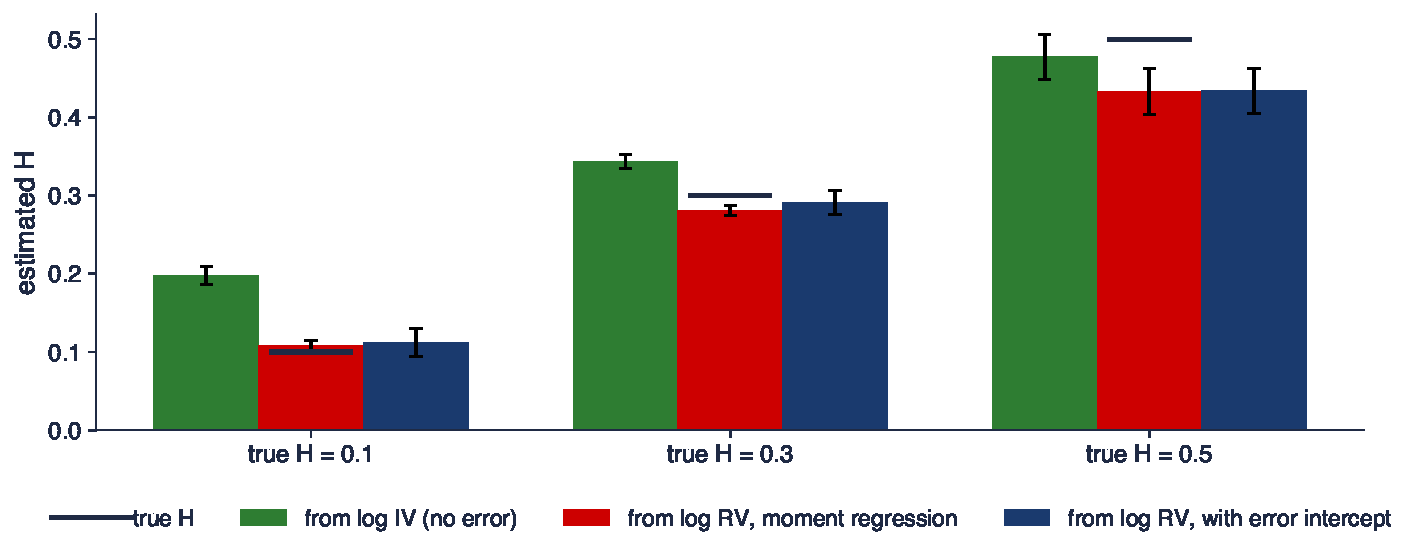
\includegraphics[width=0.97\textwidth,height=0.48\textheight,keepaspectratio]{ats_ch10_noise_sim.pdf}
\end{center}
\vspace{-0.25cm}
\begin{itemize}
    \item Logaritmul volatilității este un OU fracționar pe 78 de pași intraday pe zi, 2\,500 de zile, 8 replicări; IV zilnic (fără eroare) și RV din cele 78 de randamente pătratice; estimatorul GJR
\end{itemize}
\quantlet{ATS\_ch10\_rough}{\qlurl{ATS_ch10_rough}}
\end{frame}

\begin{frame}{Interpretarea simulării}
\itemsize{\small}
\begin{itemize}
    \item $H$ adevărat $= 0{,}1$: din IV 0{,}20, din RV 0{,}11, RV cu termen liber 0{,}11: deplasarea de integrare și cea de eroare aproape se anulează
    \item $H$ adevărat $= 0{,}5$: IV 0{,}48, RV 0{,}43, cu termen liber 0{,}43; $H$ adevărat $= 0{,}3$: 0{,}34; 0{,}28; 0{,}29
    \item Cu RV de 5 minute, eroarea este prea mică pentru a transforma $H = 0{,}5$ în valorile 0,1--0,15 observate în date
    \item Un proxy mai zgomotos (Parkinson, randamente pătratice) sau un alt model de volatilitate ar putea; concluzia depinde de această schemă
\end{itemize}
\end{frame}

\begin{frame}{Neregularitate și persistență}
\itemsize{\small}
\begin{itemize}
    \item În fBm un singur parametru le fixează pe amîndouă: $H$ mic înseamnă traiectorii neregulate și (pentru creșteri) antipersistență
    \begin{itemize}
        \item modelele Cauchy și cu nucleu gamma separă dimensiunea fractală (scări mici) de efectul Hurst (scări mari) \refGS
    \end{itemize}
    \item \refBLPb: modelul brownian semistaționar $X_t = \int_{-\infty}^tg(t - s)\,dW_s$, $g(x) \approx x^\alpha$ lîngă 0 (neregularitate, $H = \alpha + 1/2$), $g(x) \approx x^{-\beta}$ la infinit (memorie)
    \begin{itemize}
        \item rezultatul lor: logaritmul volatilității este atît neregulat ($\alpha < 0$), cît și persistent ($\beta < 1$); cele două se estimează separat
    \end{itemize}
    \item Verificarea empirică: panta variogramei la laguri scurte față de descreșterea ACF la laguri lungi
\end{itemize}
\end{frame}

\begin{frame}{Scări mici și scări mari}
\itemsize{\footnotesize}
\begin{center}
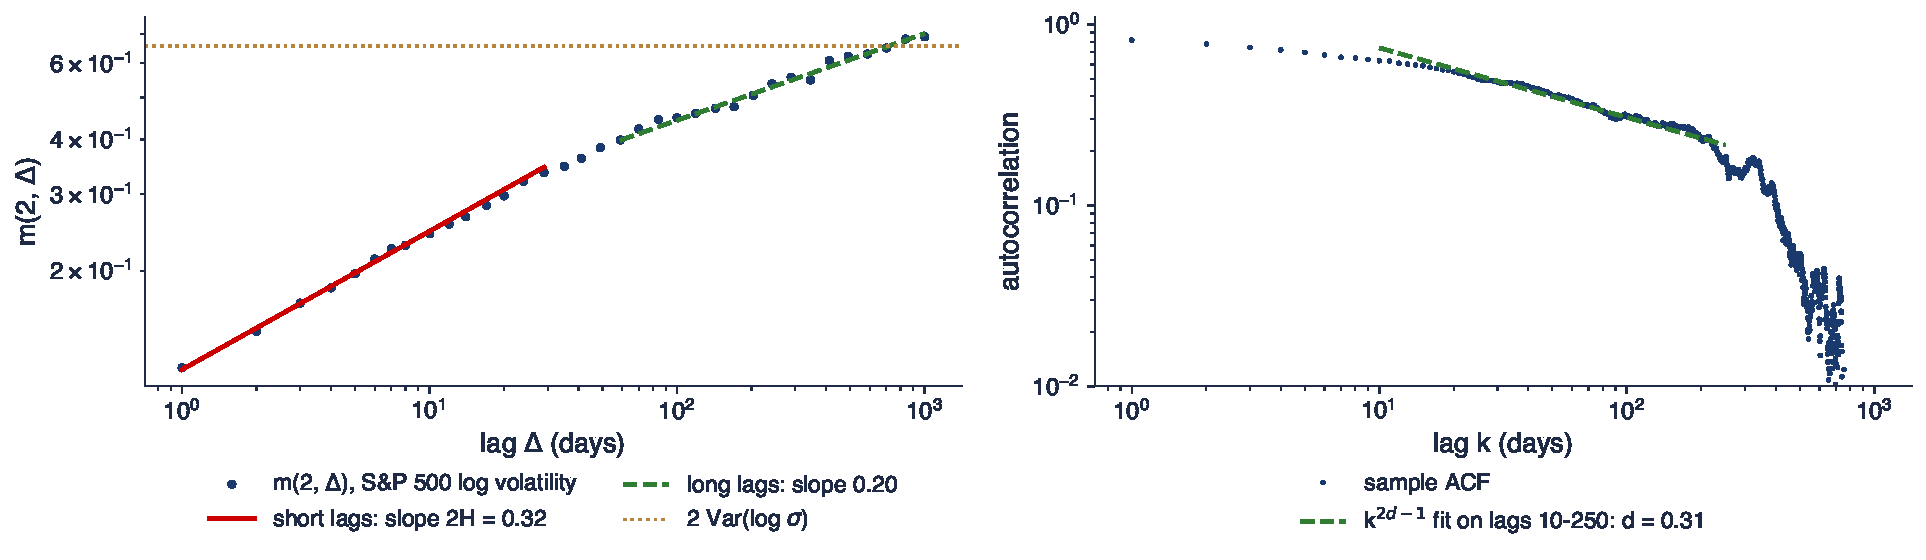
\includegraphics[width=0.97\textwidth,height=0.48\textheight,keepaspectratio]{ats_ch10_decouple.pdf}
\end{center}
\vspace{-0.25cm}
\begin{itemize}
    \item Logaritmul volatilității pentru S\&P 500, laguri 1--1000 de zile; stînga: variograma $m(2, \Delta)$ cu pantele pe lagurile 1--10 și 100--1000; dreapta: ACF de eșantion cu o ajustare $k^{2d-1}$ pe lagurile 10--250
\end{itemize}
\quantlet{ATS\_ch10\_rough}{\qlurl{ATS_ch10_rough}}
\end{frame}

\begin{frame}{Interpretarea celor două scări}
\itemsize{\small}
\begin{itemize}
    \item Laguri scurte: panta $2H = 0{,}32$, $H = 0{,}16$; laguri lungi: panta 0{,}20, încă în creștere la 1000 de zile, peste $2\Var(\log\sigma)$
    \item Citită ca proces fracționar nestaționar, panta la laguri lungi $2d - 1$ dă $d = 0{,}60$; local Whittle cu $m = 74$ dă 0{,}56
    \item Ajustarea ACF dă doar $d = 0{,}31$: ACF de eșantion este deplasată în jos cînd $d$ este aproape de 1/2 sau peste
    \item Neregulată la scări mici, foarte persistentă la scări mari: ambele afirmații sînt valabile pentru aceeași serie
\end{itemize}
\end{frame}

\begin{frame}{Recapitulare: rough volatility}
\itemsize{\small}
\begin{itemize}
    \item fBm cu $H < 1/2$: traiectorii neregulate; se simulează exact prin scufundare circulantă, versiunile Volterra prin schema hibridă
    \item Scalarea logaritmului RV dă $H \approx 0{,}1$--0,15 pe toate piețele încercate, stabil în timp
    \item Eroarea de măsurare și integrarea zilnică deplasează $\hat H$ în direcții opuse; neregularitatea și persistența sînt proprietăți separate
\end{itemize}
\end{frame}


%=============================================================================
\section{Prognoza varianței realizate: rough volatility, memorie lungă, HAR}
%=============================================================================

\begin{frame}{Predictorul RFSV (1/2)}
\itemsize{\small}
\begin{itemize}
    \item Pentru fBm (Nuzman--Poor), cu $\alpha \approx 0$, \refGJR, secțiunea 5: prognoza logaritmului varianței este o medie ponderată a trecutului său
    \[ \E[\log\sigma^2_{t+h} \mid \mathcal F_t] = \frac{\cos(H\pi)}{\pi}\,h^{H+1/2}\int_{-\infty}^t\frac{\log\sigma_s^2}{(t - s + h)(t - s)^{H+1/2}}\,ds \]
    \begin{itemize}
        \item $h$: orizontul prognozei; $\mathcal F_t$: trecutul volatilității pînă la $t$; nucleul are integrala unu, cu mai multă pondere pe trecutul recent pentru $H$ mic
        \item discretizat pe zile: $w_k = \int_k^{k+1}du/((u + h)u^{H+1/2})$, trunchiat la 500 de zile și normalizat
    \end{itemize}
\end{itemize}
\end{frame}

\begin{frame}{Predictorul RFSV (2/2): prognoza varianței}
\itemsize{\small}
\begin{itemize}
    \item De la logaritmul varianței la varianță: o corecție lognormală
    \[ \E[\sigma^2_{t+h} \mid \mathcal F_t] = \exp\big(\E[\log\sigma^2_{t+h} \mid \mathcal F_t] + 2c\nu^2h^{2H}\big) \]
    \[ c = \frac{\Gamma(3/2 - H)}{\Gamma(H + 1/2)\Gamma(2 - 2H)} \]
    \begin{itemize}
        \item $2c\nu^2h^{2H}$: jumătate din varianța condiționată a lui $\log\sigma^2_{t+h}$, care crește cu orizontul; cu valorile pentru S\&P 500, $c = 0{,}707$
    \end{itemize}
    \item Doi parametri ($H$, $\nu$), ambii din variogramă: fără verosimilitate, fără optimizare
\end{itemize}
\end{frame}

\begin{frame}{Cît de departe privesc prognozele}
\itemsize{\footnotesize}
\begin{center}
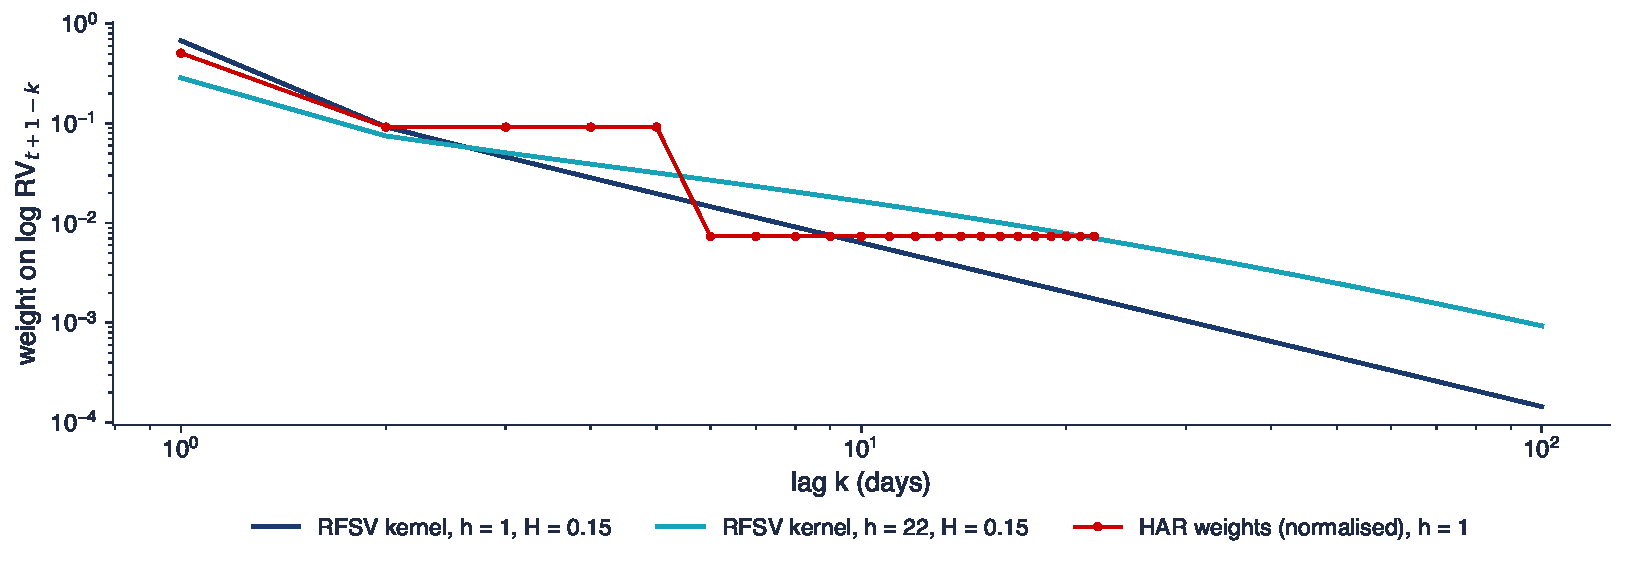
\includegraphics[width=0.97\textwidth,height=0.5\textheight,keepaspectratio]{ats_ch10_rfsv_kernel.pdf}
\end{center}
\vspace{-0.25cm}
\begin{itemize}
    \item Nucleul RFSV cu $H = 0{,}15$ (S\&P 500) pentru $h = 1$ și $h = 22$ de zile, față de ponderile HAR normalizate pentru $h = 1$
\end{itemize}
\quantlet{ATS\_ch10\_forecast}{\qlurl{ATS_ch10_forecast}}
\end{frame}

\begin{frame}{Interpretarea nucleelor}
\itemsize{\small}
\begin{itemize}
    \item $h = 1$: RFSV pune 68\% pe ultima zi, 86\% pe ultima săptămînă, 95\% pe ultima lună; HAR: 51\% și 87\%
    \item $h = 22$: doar 29\% pe ultima zi, 71\% pe ultima lună, 90\% în ultimele 100 de zile: orizonturile mai lungi privesc mai departe în trecut
    \item Nucleul își adaptează automat memoria la orizont; HAR cere o regresie separată pentru fiecare orizont
    \item RFSV nu are revenire la medie: în perioadele calme lungi nu trage prognozele spre un nivel de termen lung
\end{itemize}
\end{frame}

\begin{frame}{O comparație riguroasă în afara eșantionului}
\itemsize{\small}
\begin{itemize}
    \item Schema fixată dinainte: fereastră mobilă de 1000 de zile, parametrii reestimați la fiecare 20 de zile doar cu datele pînă la $t$; ținta $RV_{t+h}$, $h \in \{1, 5, 22\}$
    \begin{itemize}
        \item HAR: regresie directă a lui $\log RV_{t+h}$; ARFIMA$(0,d,0)$: $d$ local Whittle (limitat la 0,49), AR($\infty$) iterat; RFSV: $H$, $\nu$ din fereastră
    \end{itemize}
    \item Pierderea: QLIKE $L = RV/F - \log(RV/F) - 1$, robustă la zgomotul proxy-ului RV \refPat; și MSE al logaritmilor
    \begin{itemize}
        \item prognozele de nivel din prognoze logaritmice cer corecția lognormală: $\exp(\hat\mu + \hat s^2/2)$ pentru HAR și ARFIMA, $2c\nu^2h^{2H}$ pentru RFSV
    \end{itemize}
    \item Inferența: DM cu varianță Newey--West (\atschlink{https://danpele.github.io/Advanced-Time-Series/RO/Cursuri/capitol1_evaluarea_prognozelor.pdf}{Capitolul 1}) \refDM; diferențele de pierderi sînt ele însele persistente, deci p-value-urile sînt optimiste
\end{itemize}
\end{frame}

\begin{frame}{RFSV și ARFIMA față de HAR}
\itemsize{\footnotesize}
\begin{center}
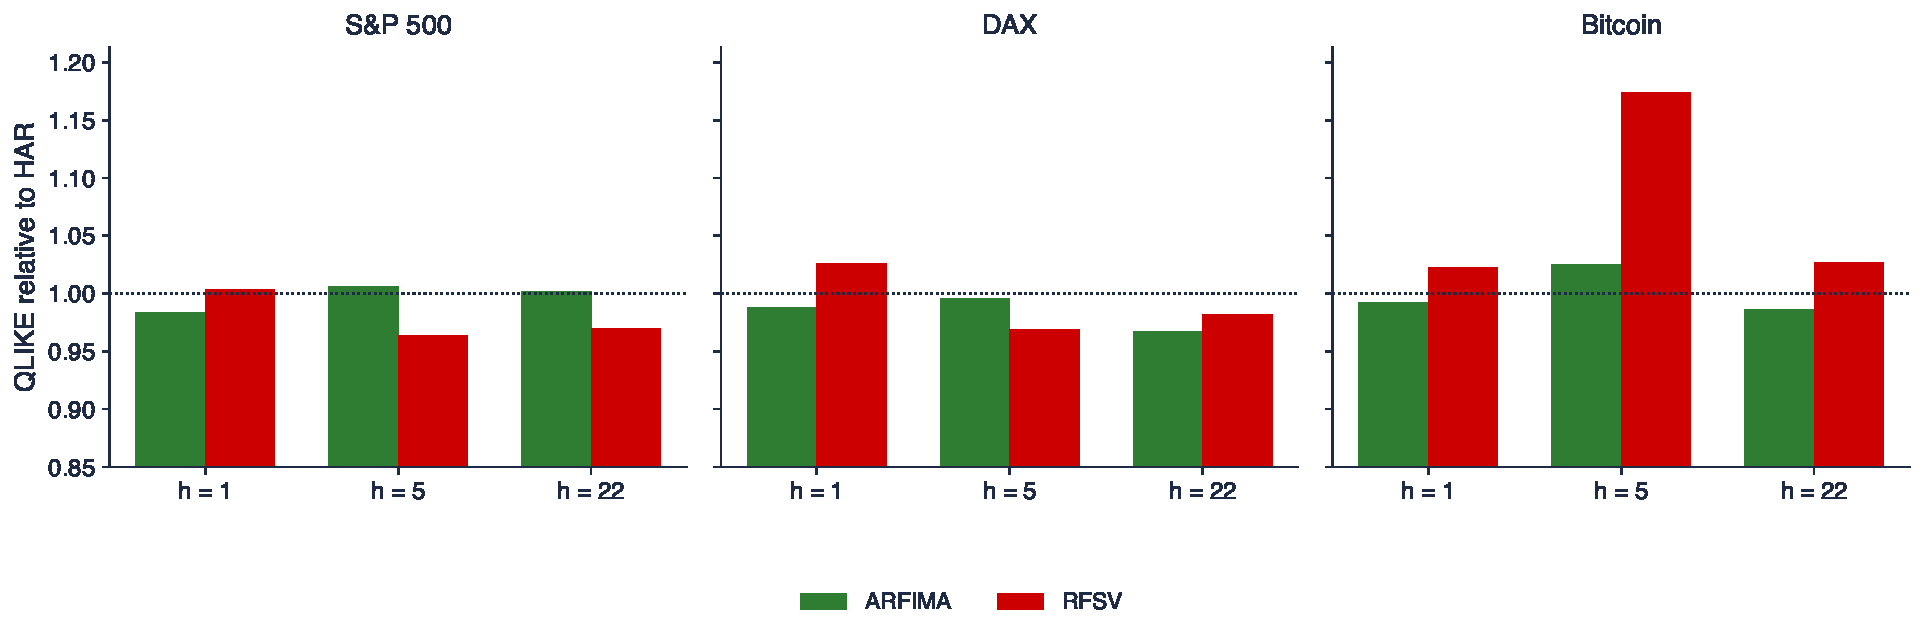
\includegraphics[width=0.97\textwidth,height=0.48\textheight,keepaspectratio]{ats_ch10_forecast.pdf}
\end{center}
\vspace{-0.25cm}
\begin{itemize}
    \item QLIKE mediu relativ la HAR (sub 1: mai bun decît HAR); o stea marchează un p-value DM sub 5\%; S\&P 500 6 ianuarie 2004 -- 24 ianuarie 2022 ($T = 4\,531$), DAX ($T = 4\,593$), Bitcoin 10 octombrie 2020 -- 27 august 2026 ($T = 2\,144$)
\end{itemize}
\quantlet{ATS\_ch10\_forecast}{\qlurl{ATS_ch10_forecast}}
\end{frame}

\begin{frame}{Interpretarea comparației prognozelor}
\itemsize{\footnotesize}
\begin{center}
\scriptsize
\begin{tabular}{lcccccc}
\toprule
\textbf{QLIKE / HAR} & \multicolumn{2}{c}{S\&P 500} & \multicolumn{2}{c}{DAX} & \multicolumn{2}{c}{Bitcoin} \\ & ARFIMA & RFSV & ARFIMA & RFSV & ARFIMA & RFSV \\
\midrule
$h = 1$ & 0{,}984 & 1{,}003 & 0{,}988 & 1{,}026 & 0{,}992 & 1{,}022 \\
$h = 5$ & 1{,}006 & 0{,}964 & 0{,}996 & 0{,}969 & 1{,}025 & 1{,}174 \\
$h = 22$ & 1{,}002 & 0{,}969 & 0{,}968 & 0{,}982 & 0{,}986 & 1{,}027 \\
\bottomrule
\end{tabular}
\end{center}
\begin{itemize}
    \item S\&P 500 și DAX: RFSV este cu 1{,}8\% pînă la 3{,}6\% mai bun decît HAR la 5 și 22 de zile, dar mai slab la o zi; DM la 5 zile: \ensuremath{-}1{,}78 ($p$ 0{,}07) și \ensuremath{-}1{,}62 ($p$ 0{,}11)
    \item Bitcoin: RFSV este mai slab la toate orizonturile (1{,}174 la 5 zile); $\hat H$ mobil variază între 0{,}04 și 0{,}15, cu mediana 0{,}08
    \item ARFIMA se află peste tot la cel mult 3{,}2\% de HAR; dintre cele 18 comparații QLIKE, niciuna este semnificativă la 5\%
    \item Neregularitatea este un fapt stilizat robust; cîștigul ei în prognoză față de HAR este mic și depinde de orizont, ca în \refGJR\ și \refWXY
\end{itemize}
\end{frame}

\begin{frame}{Recapitulare: prognoza}
\itemsize{\small}
\begin{itemize}
    \item RFSV prognozează cu un nucleu putere dependent de orizont și o corecție lognormală, din doi parametri ai variogramei
    \item În afara eșantionului, RFSV, ARFIMA și HAR sînt apropiate; RFSV cîștigă cîteva procente la orizonturi săptămînale și lunare pentru indicii bursieri
    \item Preînregistrați schema, folosiți QLIKE și tratați cu prudență p-value-urile DM cînd diferențele de pierderi sînt persistente
\end{itemize}
\end{frame}


%=============================================================================
\section{AI în descoperirea științifică}
%=============================================================================

\begin{frame}{O întrebare deschisă}
\itemsize{\small}
\begin{itemize}
    \item Este neregularitatea volatilității o proprietate a procesului de volatilitate sau a felului în care o măsurăm?
    \begin{itemize}
        \item formal: $H_0$: $H \ge 0{,}3$ pentru varianța integrată; testat cu estimatori consistenți sub eroare de măsurare, pe active, măsuri și eșantioane preînregistrate
        \item infirmată dacă estimațiile corectate rămîn sub 0,2 pentru toate frecvențele de eșantionare și piețele
    \end{itemize}
    \item Miza: modelele de tip rough volatility schimbă evaluarea opțiunilor și acoperirea; dacă neregularitatea este un artefact, modelele markoviene sînt suficiente
    \begin{itemize}
        \item literatura de pornire: \refGJR, \refFTW, \refBCPV, \refCD, \refBLPb
    \end{itemize}
\end{itemize}
\end{frame}

\begin{frame}{Bucla de cercetare cu un asistent AI}
\itemsize{\footnotesize}
\begin{itemize}
    \item Un asistent AI (un LLM precum Claude, ChatGPT, Gemini sau Copilot) accelerează fiecare etapă; Semantic Scholar și Elicit ajută la literatură
    \begin{itemize}
        \item \textbf{literatura}: \aiprompt{Listează articole recenzate din 2018 încoace care estimează exponentul Hurst al volatilității cu metode robuste la eroarea de măsurare; dă DOI-urile.} Apoi verificați fiecare DOI pe Crossref
        \item \textbf{ipoteza}: \aiprompt{Ce procese generatoare cu H = 0,5 ar face ca estimatorul momentelor pe RV de 5 minute să dea H aproape de 0,1?}
        \item \textbf{cod și replicare}: cereți regresia pe variogramă, apoi reproduceți întîi valoarea pentru S\&P 500 (0{,}149 aici) și tabelul de simulare
        \item \textbf{critica}: \aiprompt{Joacă rolul unui recenzent ostil: enumeră cum ar putea alegerea lagurilor, randamentele overnight, salturile și zgomotul de microstructură să deplaseze H.}
    \end{itemize}
    \item Raportul: ce s-a cerut, ce s-a păstrat, ce s-a respins (AI\_USE.md, AI\_ERRORS.md)
\end{itemize}
\end{frame}

\begin{frame}{Verificări necesare}
\itemsize{\small}
\begin{itemize}
    \item Fiecare referință există și spune ce se afirmă (DOI-ul funcționează, titlul coincide, rezultatul se află în lucrare)
    \item Scara este precizată: $H$ pentru fBm, $d$ pentru ARFIMA, $H = d + 1/2$ pentru seriile staționare; logaritmul volatilității sau al varianței
    \item Lățimile de bandă, lagurile și trimming-ul sînt raportate, cu estimații pe un interval de valori, nu o singură alegere convenabilă
    \item Rupturile și salturile de nivel sînt testate (Qu) înainte de a afirma memoria lungă
    \item Comparațiile prognozelor sînt în afara eșantionului, preînregistrate, cu QLIKE și DM
\end{itemize}
\end{frame}

\begin{frame}{Mini studiu de caz: cît de robust este „$H$ de ordinul 0,1”?}
\itemsize{\footnotesize}
\begin{center}
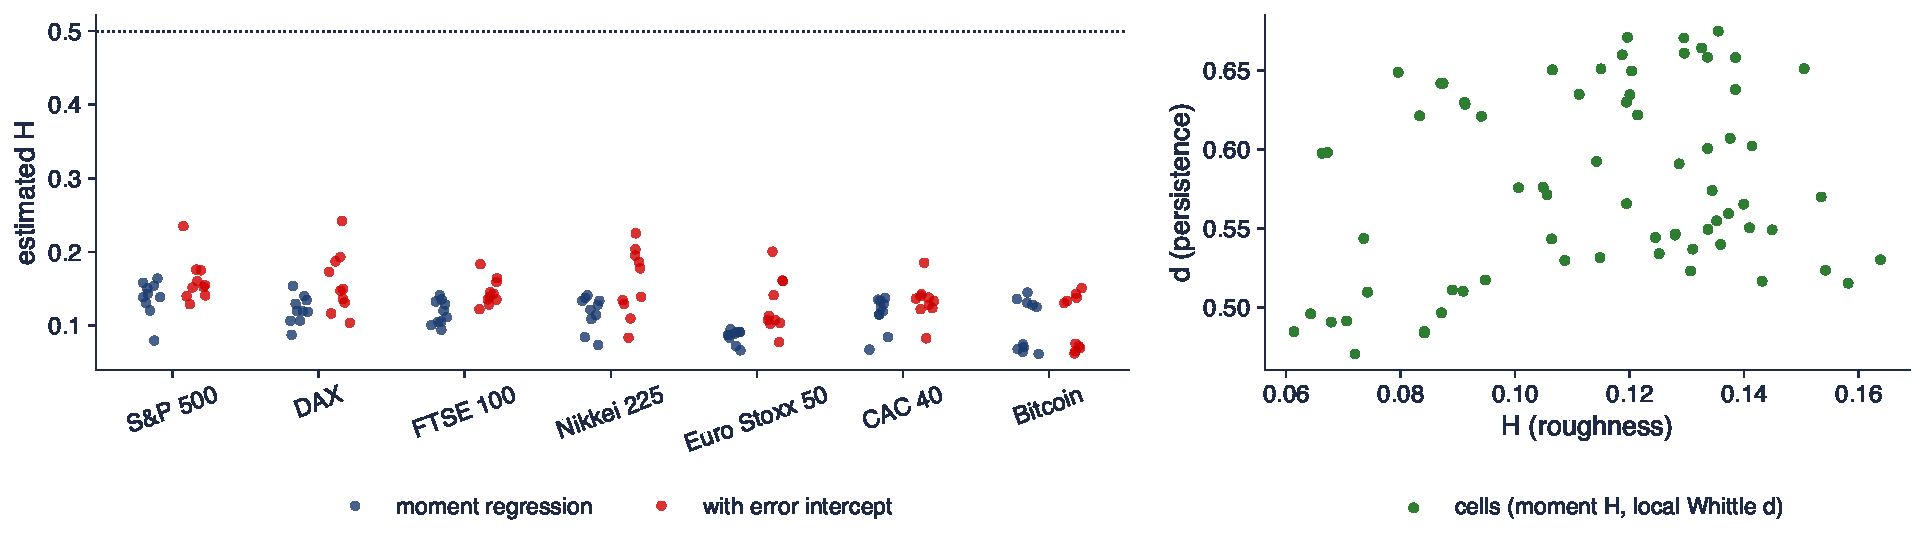
\includegraphics[width=0.97\textwidth,height=0.42\textheight,keepaspectratio]{ats_ch10_ai_case.pdf}
\end{center}
\vspace{-0.25cm}
\begin{itemize}
    \item 70 de celule: șapte active $\times$ cinci măsuri realizate $\times$ două jumătăți ale eșantionului; doi estimatori pentru fiecare (140 de estimații); dreapta: $H$ față de $d$ local Whittle din aceeași celulă
    \item $H$ între 0{,}06 și 0{,}24, mediana 0{,}13 (momente 0{,}12, cu termen liber 0{,}14); 96\% sub 0,2; $d$ între 0{,}47 și 0{,}68; corelația dintre $H$ și $d$ 0{,}24: un rezumat AI care numește volatilitatea „cu memorie scurtă pentru că $H < 1/2$” greșește
\end{itemize}
\quantlet{ATS\_ch10\_rough}{\qlurl{ATS_ch10_rough}}
\end{frame}

\begin{frame}{Idee de proiect}
\itemsize{\small}
\begin{itemize}
    \item \textbf{Neregularitatea și persistența volatilității pe piețele din Europa Centrală și de Est}: întîi replicare, apoi extindere
    \begin{itemize}
        \item replicați: \refGJR, secțiunea 2 pe datele Oxford-Man pentru S\&P 500 ($H = 0{,}149$ aici) și comparația prognozelor din secțiunea 5
        \item extindeți: date intraday pentru BET, WIG20 și EUR/RON; estimatori robuști la zgomot (FTW, GMM); teste Qu; un model BSS cu neregularitate și memorie separate
        \item preînregistrați: activele, măsurile, lagurile, lățimile de bandă, schema prognozei și pierderea
    \end{itemize}
    \item Livrabilele urmează regulile cursului: repository, raport, AI\_USE.md, AI\_ERRORS.md, susținere orală
\end{itemize}
\end{frame}


%=============================================================================
\section{Încheiere}
%=============================================================================

\begin{frame}{Idei de reținut}
\itemsize{\small}
\begin{itemize}
    \item Memoria lungă este un pol în frecvența zero; estimați-o cu local Whittle sau local Whittle exact și raportați $\hat d(m)$
    \item Salturile de nivel imită memoria lungă: testați cu Qu (2011) și urmăriți semnătura lățimii de bandă
    \item Volatilitatea este persistentă pe luni (FIGARCH, LMSV, HAR) și neregulată pe zile ($H \approx 0{,}1$)
    \item Proxy-urile contează: zgomotul scade $\hat d$ și $\hat H$; corecțiile există și trebuie raportate
    \item În prognoză, HAR rămîne un reper greu de depășit; modelele de tip rough volatility cîștigă puțin și doar la unele orizonturi
\end{itemize}
\end{frame}

\begin{frame}{Autoevaluare}
\itemsize{\small}
\begin{columns}[T]
\begin{column}{0.58\textwidth}
\begin{block}{Întrebări}
\begin{itemize}
    \item De ce este varianța asimptotică a local Whittle $1/(4m)$, iar a GPH $\pi^2/(24m)$?
    \item De ce eșuează local Whittle pentru $d > 1$ și cum corectează local Whittle exact problema?
    \item Ce formă spectrală produce un salt aleator de nivel?
    \item De ce nu este FIGARCH staționar în covarianță?
    \item Cum poate o serie să fie neregulată și cu memorie lungă în același timp?
\end{itemize}
\end{block}
\end{column}
\begin{column}{0.38\textwidth}
\begin{block}{Urmează: \atschlink{https://danpele.github.io/Advanced-Time-Series/RO/Cursuri/capitol11_analiza_spectrala_analiza_wavelet.pdf}{Capitolul 11}}
\begin{itemize}
    \item Analiză spectrală și analiză wavelet
    \item multitaper, coerență, wavelets: instrumentele de frecvență din spatele acestui capitol
\end{itemize}
\end{block}
\end{column}
\end{columns}
\end{frame}


%=============================================================================
\section{Anexă}
%=============================================================================

\begin{frame}{Anexă: varianța estimatorului local Whittle}
\hypertarget{atsapp1}{}\atsappback{atssrc1}{Înapoi}
\itemsize{\small}
\begin{itemize}
    \item Dezvoltăm $R'(\hat d) = 0$ în jurul lui $d$: $\sqrt m(\hat d - d) = -\sqrt m\,R'(d)/R''(\bar d)$
    \item $\sqrt m\,R'(d) = \dfrac{2}{\sqrt m}\sum_j\nu_j(\xi_j - 1) + o_p(1)$, $\xi_j = \lambda_j^{2d}I(\lambda_j)/G$; cu $\Var\xi_j \to 1$ și $\frac1m\sum\nu_j^2 \to 1$: $\to N(0, 4)$
    \item $R''(d) = \dfrac4m\sum_j\nu_j^2\xi_j/\bar\xi - \big(\dfrac2m\sum_j\nu_j\xi_j/\bar\xi\big)^2 \to_p 4$
    \item Deci $\sqrt m(\hat d - d) \to N(0, 4/16) = N(0, 1/4)$; la GPH aceleași ponderi înmulțesc $\log\xi_j$ cu varianța $\pi^2/6$: $N(0, \pi^2/24)$
\end{itemize}
\end{frame}

\begin{frame}{Anexă: scalarea momentelor fBm}
\hypertarget{atsapp2}{}\atsappback{atssrc2}{Înapoi}
\itemsize{\small}
\begin{itemize}
    \item $W^H_{t+\Delta} - W^H_t \sim N(0, \Delta^{2H})$, deci $\E|W^H_{t+\Delta} - W^H_t|^q = \Delta^{qH}\E|Z|^q$, $\E|Z|^q = 2^{q/2}\Gamma\big(\tfrac{q+1}{2}\big)/\sqrt\pi$
    \item Cu $\log\sigma_t = \nu W^H_t$: $\log m(q, \Delta) = q\log\nu + \log\E|Z|^q + qH\log\Delta$: panta $\zeta_q = qH$
    \item Abateri: $\zeta_q$ concav semnalează multifractalitate sau cozi groase; un termen liber în $m(2, \Delta) = \nu^2\Delta^{2H} + 2s^2$ semnalează o eroare de măsurare i.i.d.\ cu varianța $s^2$
    \item Spectrul fGn lîngă zero: $f(\lambda) \propto |\lambda|^{1-2H}$, adică creșterile sînt de tip ARFIMA cu $d = H - 1/2$
\end{itemize}
\end{frame}


%=============================================================================
\section{Bibliografie}
%=============================================================================

\begin{frame}{Bibliografie (1/4)}
\itemsize{\tiny}
\begin{itemize}
    \item Andersen, T. G., Bollerslev, T., Diebold, F. X., \& Labys, P. (2003). Modeling and forecasting realized volatility. \textit{Econometrica}, 71(2), 579--625. \href{https://doi.org/10.1111/1468-0262.00418}{doi:10.1111/1468-0262.00418}
    \item Andrews, D. W. K., \& Sun, Y. (2004). Adaptive local polynomial Whittle estimation of long-range dependence. \textit{Econometrica}, 72(2), 569--614. \href{https://doi.org/10.1111/j.1468-0262.2004.00501.x}{doi:10.1111/j.1468-0262.2004.00501.x}
    \item Baillie, R. T., Bollerslev, T., \& Mikkelsen, H. O. (1996). Fractionally integrated generalized autoregressive conditional heteroskedasticity. \textit{Journal of Econometrics}, 74(1), 3--30. \href{https://doi.org/10.1016/S0304-4076(95)01749-6}{doi:10.1016/S0304-4076(95)01749-6}
    \item Baillie, R. T., Chung, C.-F., \& Tieslau, M. A. (1996). Analysing inflation by the fractionally integrated ARFIMA--GARCH model. \textit{Journal of Applied Econometrics}, 11(1), 23--40. \href{https://doi.org/10.1002/(SICI)1099-1255(199601)11:1\%3C23::AID-JAE374\%3E3.0.CO;2-M}{doi:10.1002/(SICI)1099-1255(199601)11:1\textless{}23::AID-JAE374\textgreater{}3.0.CO;2-M}
    \item Bandi, F. M., \& Perron, B. (2006). Long memory and the relation between implied and realized volatility. \textit{Journal of Financial Econometrics}, 4(4), 636--670. \href{https://doi.org/10.1093/jjfinec/nbl003}{doi:10.1093/jjfinec/nbl003}
    \item Bayer, C., Friz, P., \& Gatheral, J. (2016). Pricing under rough volatility. \textit{Quantitative Finance}, 16(6), 887--904. \href{https://doi.org/10.1080/14697688.2015.1099717}{doi:10.1080/14697688.2015.1099717}
    \item Bennedsen, M., Lunde, A., \& Pakkanen, M. S. (2022). Decoupling the short- and long-term behavior of stochastic volatility. \textit{Journal of Financial Econometrics}, 20(5), 961--1006. \href{https://doi.org/10.1093/jjfinec/nbaa049}{doi:10.1093/jjfinec/nbaa049}
    \item Bennedsen, M., Lunde, A., \& Pakkanen, M. S. (2017). Hybrid scheme for Brownian semistationary processes. \textit{Finance and Stochastics}, 21(4), 931--965. \href{https://doi.org/10.1007/s00780-017-0335-5}{doi:10.1007/s00780-017-0335-5}
    \item Beran, J., Feng, Y., Ghosh, S., \& Kulik, R. (2013). \textit{Long-Memory Processes: Probabilistic Properties and Statistical Methods}. Springer. \href{https://doi.org/10.1007/978-3-642-35512-7}{doi:10.1007/978-3-642-35512-7}
    \item Bolko, A. E., Christensen, K., Pakkanen, M. S., \& Veliyev, B. (2023). A GMM approach to estimate the roughness of stochastic volatility. \textit{Journal of Econometrics}, 235(2), 745--778. \href{https://doi.org/10.1016/j.jeconom.2022.06.009}{doi:10.1016/j.jeconom.2022.06.009}
    \item Breidt, F. J., Crato, N., \& de Lima, P. (1998). The detection and estimation of long memory in stochastic volatility. \textit{Journal of Econometrics}, 83(1--2), 325--348. \href{https://doi.org/10.1016/S0304-4076(97)00072-9}{doi:10.1016/S0304-4076(97)00072-9}
    \item Christensen, B. J., \& Nielsen, M. Ø. (2006). Asymptotic normality of narrow-band least squares in the stationary fractional cointegration model and volatility forecasting. \textit{Journal of Econometrics}, 133(1), 343--371. \href{https://doi.org/10.1016/j.jeconom.2005.03.018}{doi:10.1016/j.jeconom.2005.03.018}
    \item Comte, F., \& Renault, E. (1998). Long memory in continuous-time stochastic volatility models. \textit{Mathematical Finance}, 8(4), 291--323. \href{https://doi.org/10.1111/1467-9965.00057}{doi:10.1111/1467-9965.00057}
    \item Cont, R., \& Das, P. (2024). Rough volatility: Fact or artefact? \textit{Sankhya B}, 86(1), 191--223. \href{https://doi.org/10.1007/s13571-024-00322-2}{doi:10.1007/s13571-024-00322-2}
\end{itemize}
\end{frame}

\begin{frame}{Bibliografie (2/4)}
\itemsize{\tiny}
\begin{itemize}
    \item Corsi, F. (2009). A simple approximate long-memory model of realized volatility. \textit{Journal of Financial Econometrics}, 7(2), 174--196. \href{https://doi.org/10.1093/jjfinec/nbp001}{doi:10.1093/jjfinec/nbp001}
    \item Davidson, J. (2004). Moment and memory properties of linear conditional heteroscedasticity models, and a new model. \textit{Journal of Business \& Economic Statistics}, 22(1), 16--29. \href{https://doi.org/10.1198/073500103288619359}{doi:10.1198/073500103288619359}
    \item Davies, R. B., \& Harte, D. S. (1987). Tests for Hurst effect. \textit{Biometrika}, 74(1), 95--101. \href{https://doi.org/10.1093/biomet/74.1.95}{doi:10.1093/biomet/74.1.95}
    \item Diebold, F. X., \& Inoue, A. (2001). Long memory and regime switching. \textit{Journal of Econometrics}, 105(1), 131--159. \href{https://doi.org/10.1016/S0304-4076(01)00073-2}{doi:10.1016/S0304-4076(01)00073-2}
    \item Diebold, F. X., \& Mariano, R. S. (1995). Comparing predictive accuracy. \textit{Journal of Business \& Economic Statistics}, 13(3), 253--263. \href{https://doi.org/10.1080/07350015.1995.10524599}{doi:10.1080/07350015.1995.10524599}
    \item Dietrich, C. R., \& Newsam, G. N. (1997). Fast and exact simulation of stationary Gaussian processes through circulant embedding of the covariance matrix. \textit{SIAM Journal on Scientific Computing}, 18(4), 1088--1107. \href{https://doi.org/10.1137/S1064827592240555}{doi:10.1137/S1064827592240555}
    \item El Euch, O., \& Rosenbaum, M. (2019). The characteristic function of rough Heston models. \textit{Mathematical Finance}, 29(1), 3--38. \href{https://doi.org/10.1111/mafi.12173}{doi:10.1111/mafi.12173}
    \item Fox, R., \& Taqqu, M. S. (1986). Large-sample properties of parameter estimates for strongly dependent stationary Gaussian time series. \textit{The Annals of Statistics}, 14(2), 517--532. \href{https://doi.org/10.1214/aos/1176349936}{doi:10.1214/aos/1176349936}
    \item Fukasawa, M., Takabatake, T., \& Westphal, R. (2022). Consistent estimation for fractional stochastic volatility model under high-frequency asymptotics. \textit{Mathematical Finance}, 32(4), 1086--1132. \href{https://doi.org/10.1111/mafi.12354}{doi:10.1111/mafi.12354}
    \item Gatheral, J., Jaisson, T., \& Rosenbaum, M. (2018). Volatility is rough. \textit{Quantitative Finance}, 18(6), 933--949. \href{https://doi.org/10.1080/14697688.2017.1393551}{doi:10.1080/14697688.2017.1393551}
    \item Geweke, J., \& Porter-Hudak, S. (1983). The estimation and application of long memory time series models. \textit{Journal of Time Series Analysis}, 4(4), 221--238. \href{https://doi.org/10.1111/j.1467-9892.1983.tb00371.x}{doi:10.1111/j.1467-9892.1983.tb00371.x}
    \item Gneiting, T., \& Schlather, M. (2004). Stochastic models that separate fractal dimension and the Hurst effect. \textit{SIAM Review}, 46(2), 269--282. \href{https://doi.org/10.1137/S0036144501394387}{doi:10.1137/S0036144501394387}
    \item Granger, C. W. J., \& Hyung, N. (2004). Occasional structural breaks and long memory with an application to the S\&P 500 absolute stock returns. \textit{Journal of Empirical Finance}, 11(3), 399--421. \href{https://doi.org/10.1016/j.jempfin.2003.03.001}{doi:10.1016/j.jempfin.2003.03.001}
    \item Granger, C. W. J., \& Joyeux, R. (1980). An introduction to long-memory time series models and fractional differencing. \textit{Journal of Time Series Analysis}, 1(1), 15--29. \href{https://doi.org/10.1111/j.1467-9892.1980.tb00297.x}{doi:10.1111/j.1467-9892.1980.tb00297.x}
\end{itemize}
\end{frame}

\begin{frame}{Bibliografie (3/4)}
\itemsize{\tiny}
\begin{itemize}
    \item Granger, C. W. J. (1980). Long memory relationships and the aggregation of dynamic models. \textit{Journal of Econometrics}, 14(2), 227--238. \href{https://doi.org/10.1016/0304-4076(80)90092-5}{doi:10.1016/0304-4076(80)90092-5}
    \item Hassler, U., \& Wolters, J. (1995). Long memory in inflation rates: International evidence. \textit{Journal of Business \& Economic Statistics}, 13(1), 37--45. \href{https://doi.org/10.1080/07350015.1995.10524577}{doi:10.1080/07350015.1995.10524577}
    \item Heber, G., Lunde, A., Shephard, N., \& Sheppard, K. K. (2009). Oxford-Man Institute\'s realized library, version 0.3. Oxford-Man Institute, University of Oxford. \href{https://web.archive.org/web/20220301022212/https://realized.oxford-man.ox.ac.uk/}{web.archive.org}
    \item Henry, M., \& Robinson, P. M. (1996). Bandwidth choice in Gaussian semiparametric estimation of long range dependence. In \textit{Athens Conference on Applied Probability and Time Series Analysis}, Lecture Notes in Statistics 115, 220--232. Springer. \href{https://doi.org/10.1007/978-1-4612-2412-9_16}{doi:10.1007/978-1-4612-2412-9\_16}
    \item Hosking, J. R. M. (1981). Fractional differencing. \textit{Biometrika}, 68(1), 165--176. \href{https://doi.org/10.1093/biomet/68.1.165}{doi:10.1093/biomet/68.1.165}
    \item Hurst, H. E. (1951). Long-term storage capacity of reservoirs. \textit{Transactions of the American Society of Civil Engineers}, 116(1), 770--799. \href{https://doi.org/10.1061/TACEAT.0006518}{doi:10.1061/TACEAT.0006518}
    \item Hurvich, C. M., Deo, R., \& Brodsky, J. (1998). The mean squared error of Geweke and Porter-Hudak\'s estimator of the memory parameter of a long-memory time series. \textit{Journal of Time Series Analysis}, 19(1), 19--46. \href{https://doi.org/10.1111/1467-9892.00075}{doi:10.1111/1467-9892.00075}
    \item Hurvich, C. M., Moulines, E., \& Soulier, P. (2005). Estimating long memory in volatility. \textit{Econometrica}, 73(4), 1283--1328. \href{https://doi.org/10.1111/j.1468-0262.2005.00616.x}{doi:10.1111/j.1468-0262.2005.00616.x}
    \item Johansen, S., \& Nielsen, M. Ø. (2012). Likelihood inference for a fractionally cointegrated vector autoregressive model. \textit{Econometrica}, 80(6), 2667--2732. \href{https://doi.org/10.3982/ECTA9299}{doi:10.3982/ECTA9299}
    \item Livieri, G., Mouti, S., Pallavicini, A., \& Rosenbaum, M. (2018). Rough volatility: Evidence from option prices. \textit{IISE Transactions}, 50(9), 767--776. \href{https://doi.org/10.1080/24725854.2018.1444297}{doi:10.1080/24725854.2018.1444297}
    \item Lu, Y. K., \& Perron, P. (2010). Modeling and forecasting stock return volatility using a random level shift model. \textit{Journal of Empirical Finance}, 17(1), 138--156. \href{https://doi.org/10.1016/j.jempfin.2009.10.001}{doi:10.1016/j.jempfin.2009.10.001}
    \item MacKinnon, J. G., \& Nielsen, M. Ø. (2014). Numerical distribution functions of fractional unit root and cointegration tests. \textit{Journal of Applied Econometrics}, 29(1), 161--171. \href{https://doi.org/10.1002/jae.2295}{doi:10.1002/jae.2295}
    \item Mandelbrot, B. B., \& Van Ness, J. W. (1968). Fractional Brownian motions, fractional noises and applications. \textit{SIAM Review}, 10(4), 422--437. \href{https://doi.org/10.1137/1010093}{doi:10.1137/1010093}
    \item Nielsen, M. Ø., \& Shimotsu, K. (2007). Determining the cointegrating rank in nonstationary fractional systems by the exact local Whittle approach. \textit{Journal of Econometrics}, 141(2), 574--596. \href{https://doi.org/10.1016/j.jeconom.2006.10.008}{doi:10.1016/j.jeconom.2006.10.008}
\end{itemize}
\end{frame}

\begin{frame}{Bibliografie (4/4)}
\itemsize{\tiny}
\begin{itemize}
    \item Parkinson, M. (1980). The extreme value method for estimating the variance of the rate of return. \textit{The Journal of Business}, 53(1), 61--65. \href{https://doi.org/10.1086/296071}{doi:10.1086/296071}
    \item Patton, A. J. (2011). Volatility forecast comparison using imperfect volatility proxies. \textit{Journal of Econometrics}, 160(1), 246--256. \href{https://doi.org/10.1016/j.jeconom.2010.03.034}{doi:10.1016/j.jeconom.2010.03.034}
    \item Perron, P., \& Qu, Z. (2010). Long-memory and level shifts in the volatility of stock market return indices. \textit{Journal of Business \& Economic Statistics}, 28(2), 275--290. \href{https://doi.org/10.1198/jbes.2009.06171}{doi:10.1198/jbes.2009.06171}
    \item Petropoulos, F., Apiletti, D., Assimakopoulos, V., Babai, M. Z., et al.\ (2022). Forecasting: Theory and practice. \textit{International Journal of Forecasting}, 38(3), 705--871. \href{https://doi.org/10.1016/j.ijforecast.2021.11.001}{doi:10.1016/j.ijforecast.2021.11.001}
    \item Phillips, P. C. B., \& Shimotsu, K. (2004). Local Whittle estimation in nonstationary and unit root cases. \textit{The Annals of Statistics}, 32(2), 656--692. \href{https://doi.org/10.1214/009053604000000139}{doi:10.1214/009053604000000139}
    \item Qu, Z. (2011). A test against spurious long memory. \textit{Journal of Business \& Economic Statistics}, 29(3), 423--438. \href{https://doi.org/10.1198/jbes.2010.09153}{doi:10.1198/jbes.2010.09153}
    \item Robinson, P. M. (1995a). Log-periodogram regression of time series with long range dependence. \textit{The Annals of Statistics}, 23(3), 1048--1072. \href{https://doi.org/10.1214/aos/1176324636}{doi:10.1214/aos/1176324636}
    \item Robinson, P. M. (1995b). Gaussian semiparametric estimation of long range dependence. \textit{The Annals of Statistics}, 23(5), 1630--1661. \href{https://doi.org/10.1214/aos/1176324317}{doi:10.1214/aos/1176324317}
    \item Robinson, P. M. (1994). Semiparametric analysis of long-memory time series. \textit{The Annals of Statistics}, 22(1), 515--539. \href{https://doi.org/10.1214/aos/1176325382}{doi:10.1214/aos/1176325382}
    \item Shimotsu, K. (2010). Exact local Whittle estimation of fractional integration with unknown mean and time trend. \textit{Econometric Theory}, 26(2), 501--540. \href{https://doi.org/10.1017/S0266466609100075}{doi:10.1017/S0266466609100075}
    \item Shimotsu, K., \& Phillips, P. C. B. (2005). Exact local Whittle estimation of fractional integration. \textit{The Annals of Statistics}, 33(4), 1890--1933. \href{https://doi.org/10.1214/009053605000000309}{doi:10.1214/009053605000000309}
    \item Velasco, C. (1999). Gaussian semiparametric estimation of non-stationary time series. \textit{Journal of Time Series Analysis}, 20(1), 87--127. \href{https://doi.org/10.1111/1467-9892.00127}{doi:10.1111/1467-9892.00127}
    \item Wang, X., Xiao, W., \& Yu, J. (2023). Modeling and forecasting realized volatility with the fractional Ornstein--Uhlenbeck process. \textit{Journal of Econometrics}, 232(2), 389--415. \href{https://doi.org/10.1016/j.jeconom.2021.08.001}{doi:10.1016/j.jeconom.2021.08.001}
\end{itemize}
\end{frame}

\end{document}
